\documentclass[12pt, a4paper]{article}
\usepackage{graphicx}
\usepackage[a4paper, total={6in, 8in}]{geometry}
\usepackage{setspace}
\usepackage{parskip}
\usepackage{float}
\usepackage{amsmath}
\usepackage{subfig}
\usepackage[numbered]{matlab-prettifier}

\begin{document}

\graphicspath{{./images}}

\begin{center}
    \onehalfspacing
    {\Large \textbf{King Fahd University of Petroleum and Minerals} }\\ 
    {\large \textbf{
    College of Computing and Mathematics\\
    Computer Engineering Department 
    } } 
\end{center} 

\begin{figure}[h]
    \centering
    
\includegraphics[width=200px]{images/KFUPM_LOGO.png}
\end{figure}

\begin{center}\onehalfspacing
    \large \textbf{COE 588- Modeling \& Simulation \\of computer and networks Systems }\\
    \normalsize \textbf{Term 232} \\
    \large \textbf{Progress Report}\\
    \textbf{Project}: Simulation and evaluation of M/M/c \\ with an infinite buffer 
\end{center}
\vspace{1em}
\large
\begin{center}
\bgroup
\def\arraystretch{1.3}
\begin{tabular}{|c|c|}
    \hline
    \textbf{Name} & \textbf{KFUPM ID} \\
    \hline
    Hashim Al-Sadah & 201578370\\
    \hline
    Abdulwahab Alghamdi & 201734070\\
    \hline
    Hussain Al-Sinan & 202205120\\
    \hline 
\end{tabular}
\egroup
\end{center}
\vspace{1em}
\begin{center}
    \textbf{Instructor:} Dr. Ashraf S. Hasan Mahmoud.
\end{center}
\normalsize


\onehalfspacing

\section{Objective}
To simulate the multiple servers queueing system with an infinite buffer, M/M/c, 
and verify that the simulation results match with the theoretical ones. 
The average total time, average waiting time, average number of customers in the system, 
average number of customers in the buffer, and the probability of waiting will 
be simulated as function of the traffic intensity. 
Additionally, the (Probability Density Function) PDF of the total time spent in the system, 
the PDF of the waiting time in the buffer, 
and the (Probability Mass Function) PMF of the number of customers in the system will 
be obtained empirically for low, medium, and high traffic intensity. Finally, we will 
study the effect of increasing the number of servers on the probability of waiting for a fixed
traffic intensity. All the results obtained through simulation will be compared against
the theoretical ones.

\section{Theoretical Background}
The state diagram for M/M/c is shown in Figure \ref{state_diagram_MMc}. The 
number of servers is denoted by $c$, the arrival rate is $\lambda$, and the 
service rate when the system at some state $s$ is $min(s\mu, c\mu)$.

\begin{figure}[H]
  \centering 
  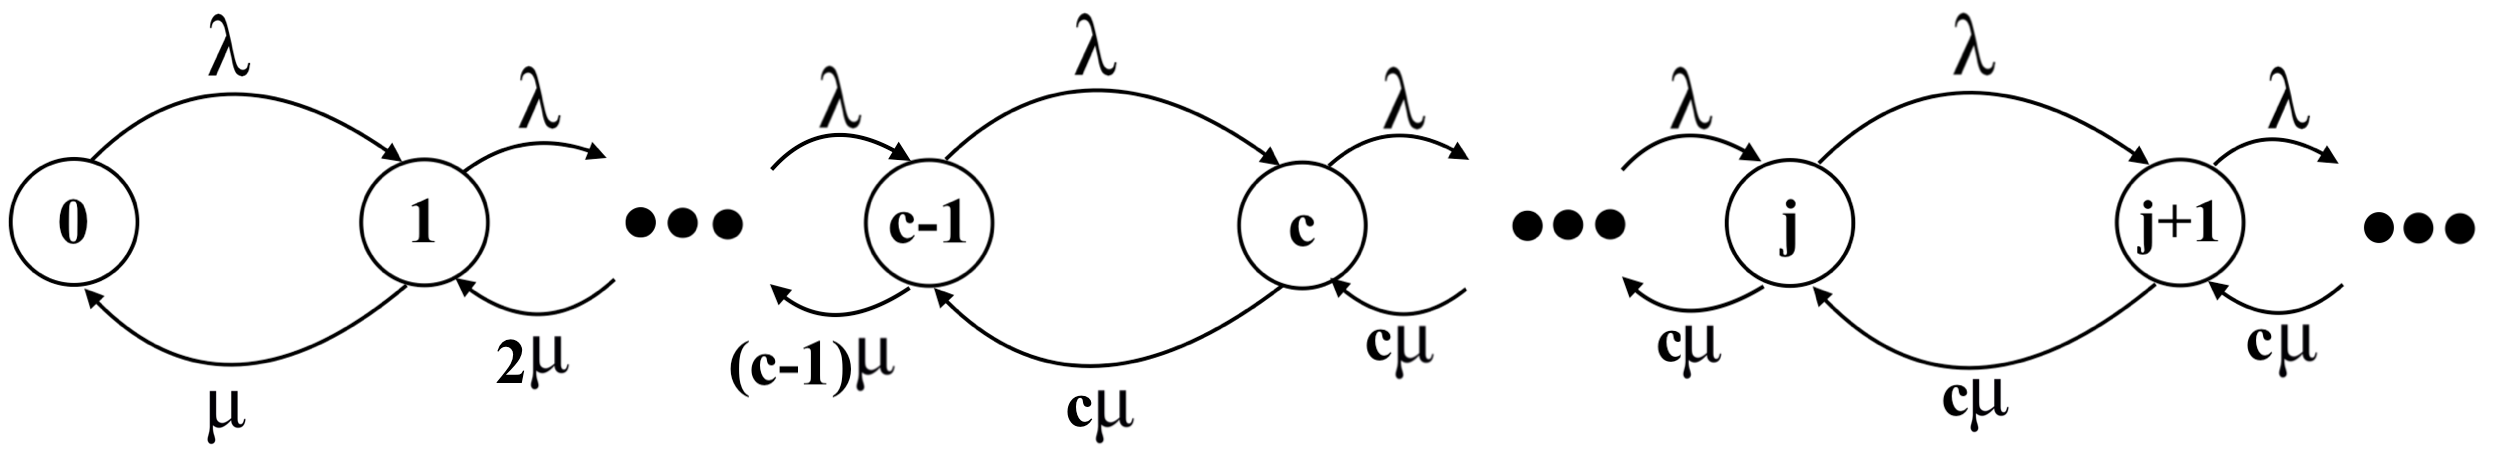
\includegraphics[width=430px]{images/MMc_state_diagram.png}
  \caption{State diagram of M/M/c}
  \label{state_diagram_MMc}
\end{figure}

From the state diagram, one can obtain the global equations and derive 
the equations that describe M/M/c. We will state the equations here without
derivation.

Define $a = \lambda / \mu$. Then the traffic intensity $\rho$ is 
\begin{equation}
  \rho = \frac{a}{c} = \frac{\lambda}{c \mu}
\end{equation}
For all the following equations, we assume that the system is stable. That is 
$\rho < 1$. Then the PMF of $N(t)$ is 
\begin{equation}
  p_0 = \left\{ 
    \left( \sum_{j=0}^{c-1} \frac{a^j}{j!} \right)  
    + \frac{a^c}{c!} \frac{1}{1 - \rho}
    \right\}^{-1}
\end{equation}
\begin{equation}
  p_j = \frac{a^j}{j!} p_0, \quad j = 1, 2, \dots, c
\end{equation}
\begin{equation}
  p_j = \frac{\rho^{j-c}}{c!} a^c p_0, \quad j = c+1, c+2, \dots 
\end{equation}

The probability of having to wait is 
\begin{equation}
  \text{Prob}[\, W > 0 \,] = \text{Prob}[\, N(t) > c \,]
  = \frac{p_c}{1 - \rho}
\end{equation}

The average buffer size is 
\begin{equation}
  E[N_q] = \left( \frac{\rho}{1 - \rho} \right) \text{Prob}
  [\, W > 0 \,]
\end{equation}

The average waiting time is 
\begin{equation}
  E[W] =\frac{E[N_q]}{\lambda}
\end{equation}

The average total time is 
\begin{equation}
  E[T] = E[W] + \frac{1}{\mu}
\end{equation}

The average number of customers in the system 
\begin{equation}
  E[N(t)] = \lambda E[T] = E[N_q] + a  
\end{equation}

The PDF and the CDF of the waiting time, respectively, are 
\begin{equation}
  f_W(t) = c \mu p_c e^{-c \mu \left( 1 - \rho \right)t}, \quad t > 0
\end{equation}
\begin{equation}
  F_W(t) = 1 - \frac{p_c}{1 - \rho} e^{-c \mu \left( 1 - \rho \right)t}, \quad t > 0
\end{equation}

The PDF of the total time is 
\begin{equation}
  f_T(t) = \frac{1}{E[T]} e^{- t/ E[T] }, \quad t \ge 0 
\end{equation}

\section{Simulation Details}

\newpage
\section{Results and Discussion}
\subsection{$E[T], E[W], E[N]$, and  $E[N_q]$}
\begin{figure}[H]
  \centering
  \subfloat[]{
    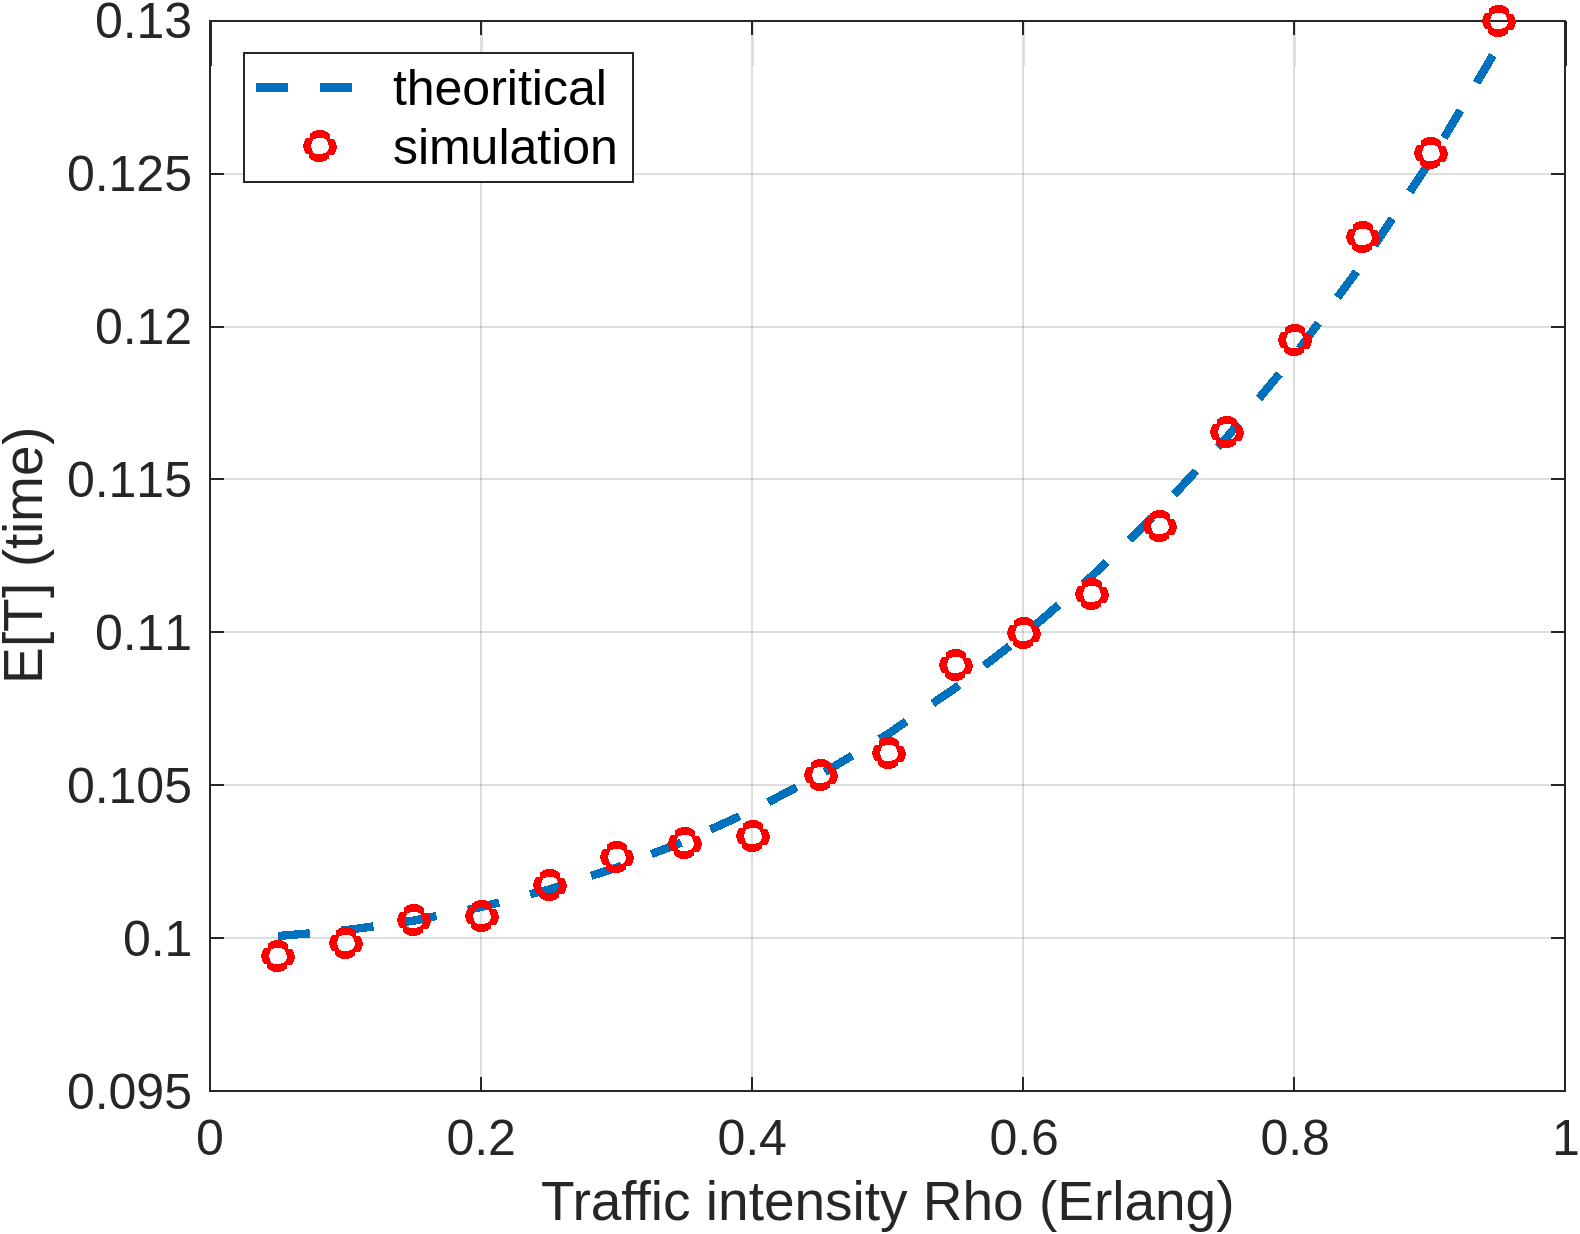
\includegraphics[width=200px]{../code/figures/avgs_vs_traffic_intensity/E_T.png}
  }  
  \subfloat[]{
    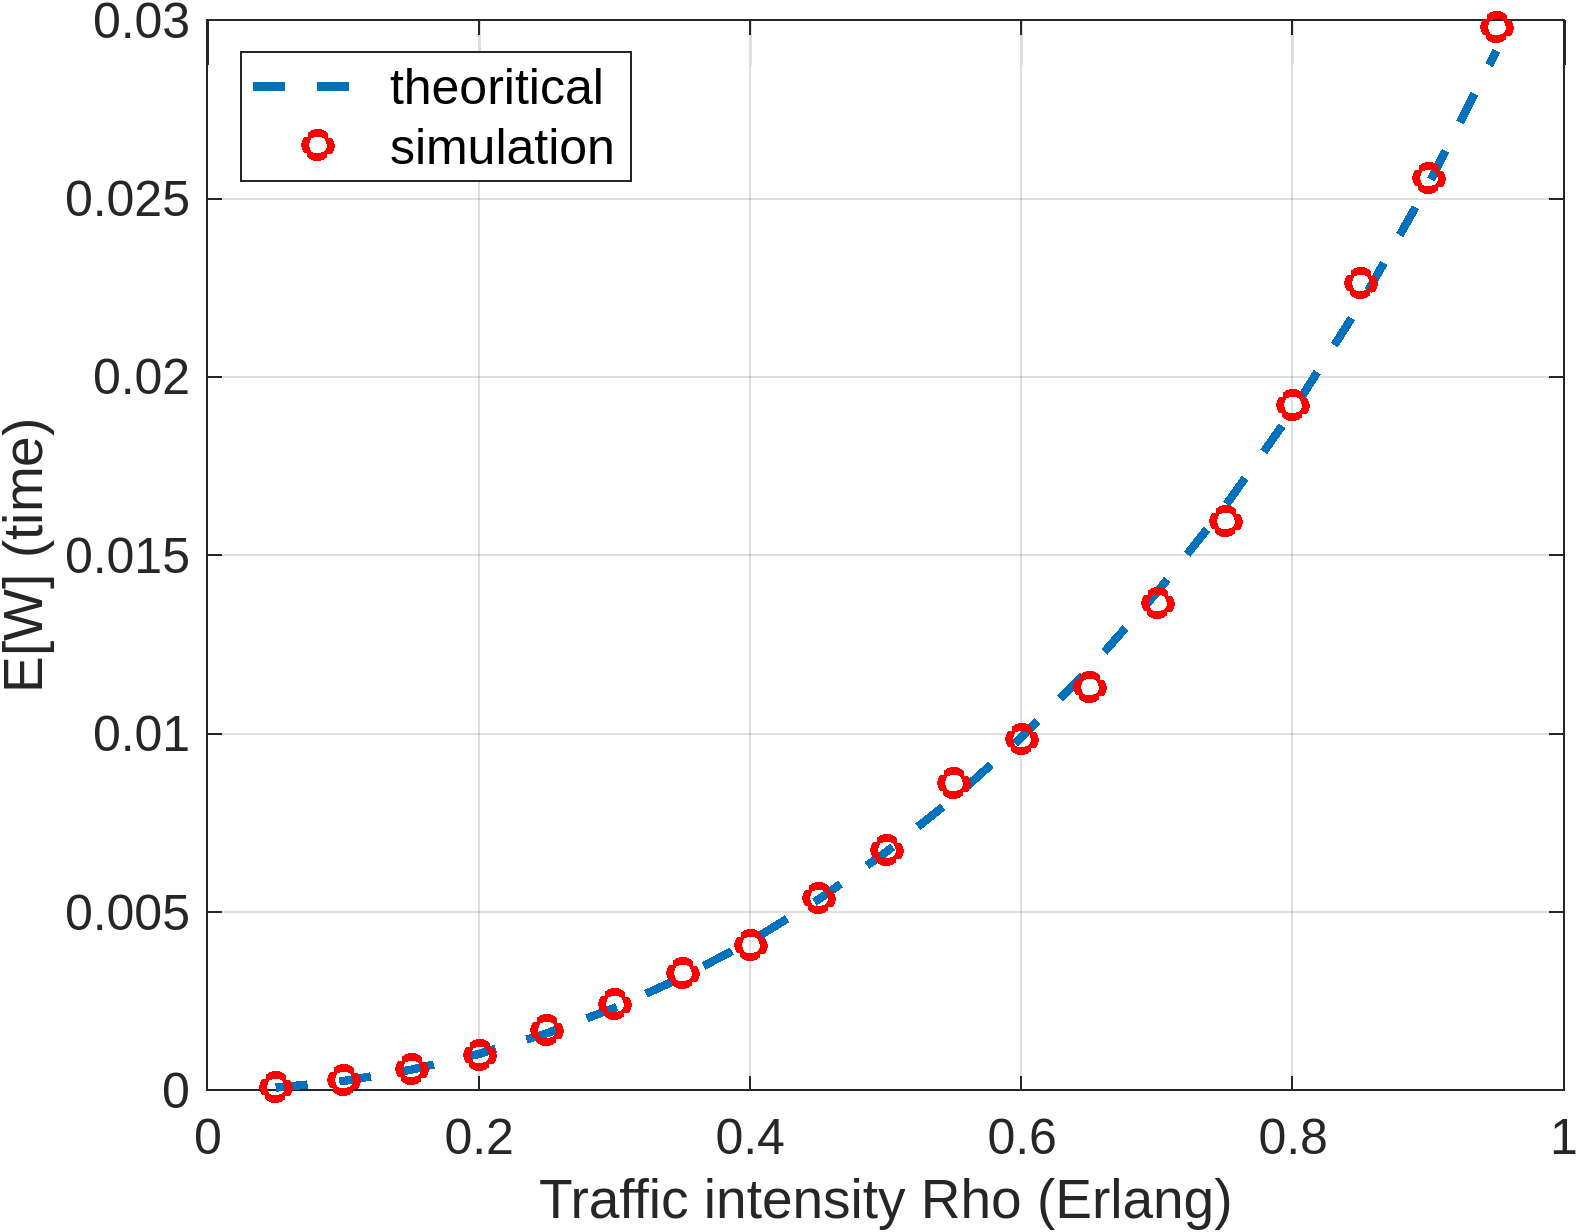
\includegraphics[width=200px]{../code/figures/avgs_vs_traffic_intensity/E_W.png}
  } 
  \hspace{0px}
  \subfloat[]{
    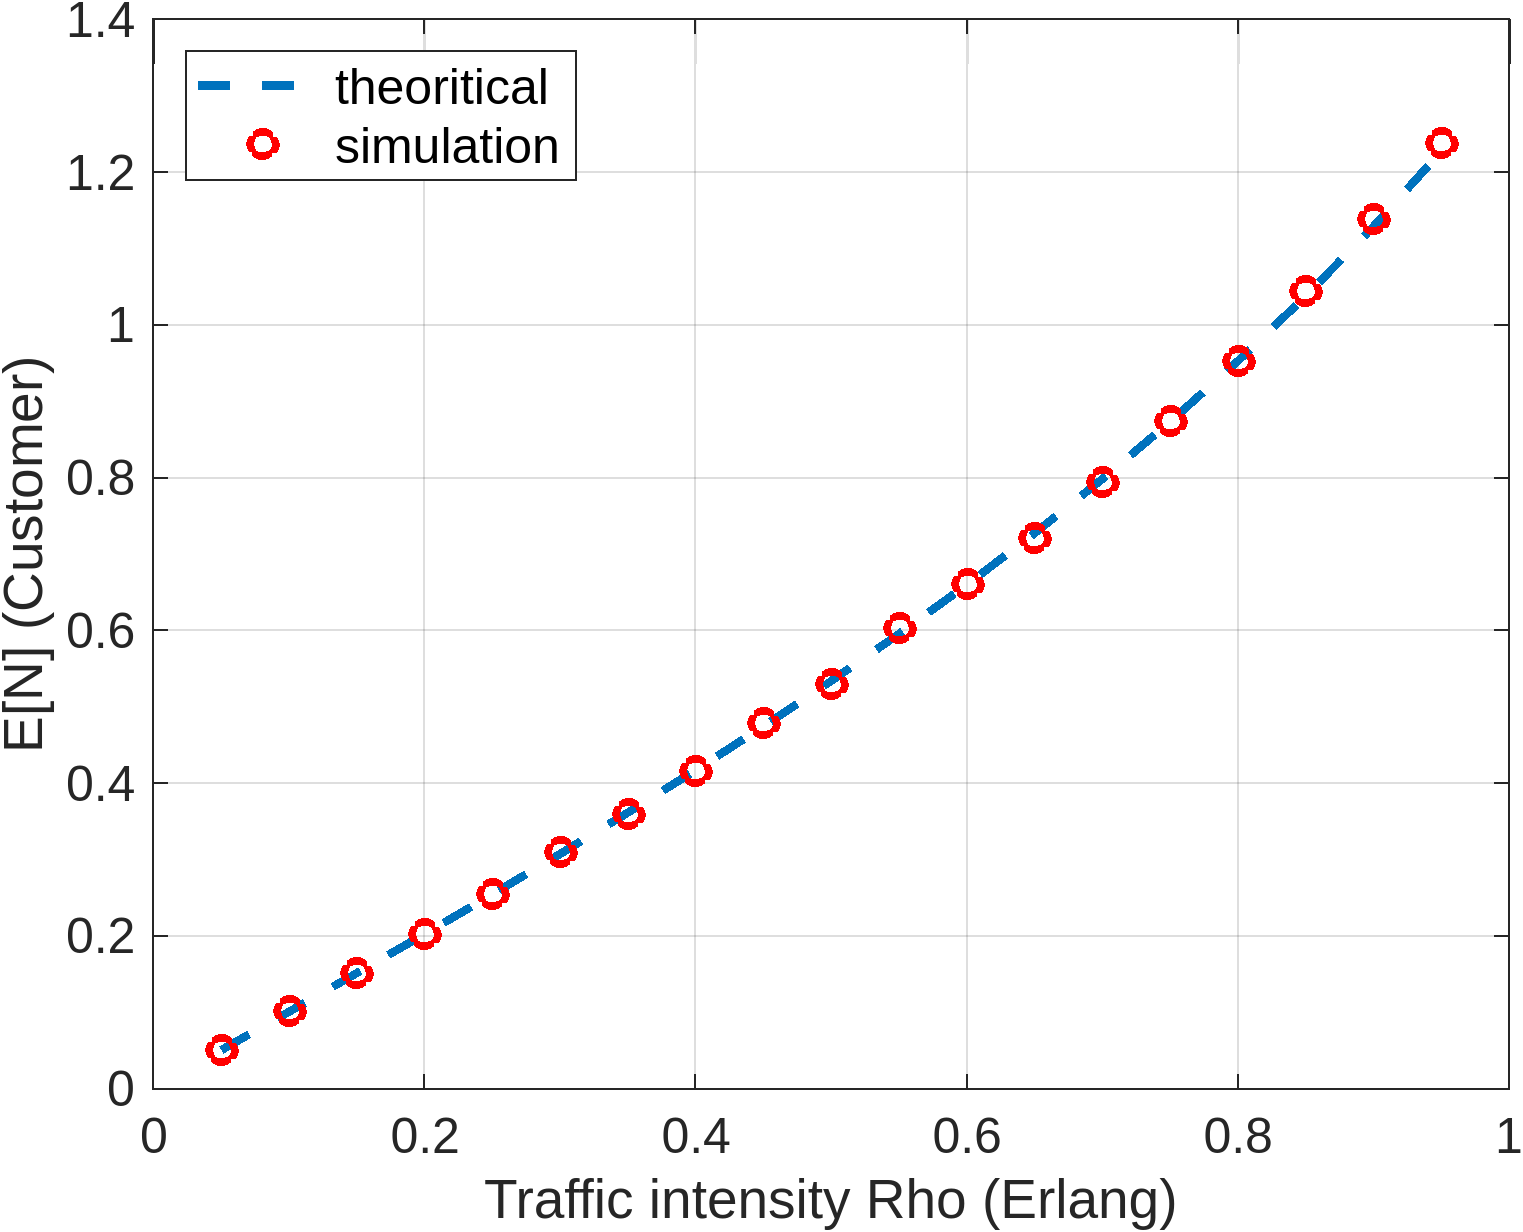
\includegraphics[width=200px]{../code/figures/avgs_vs_traffic_intensity/E_N.png}
  } 
  \subfloat[]{
    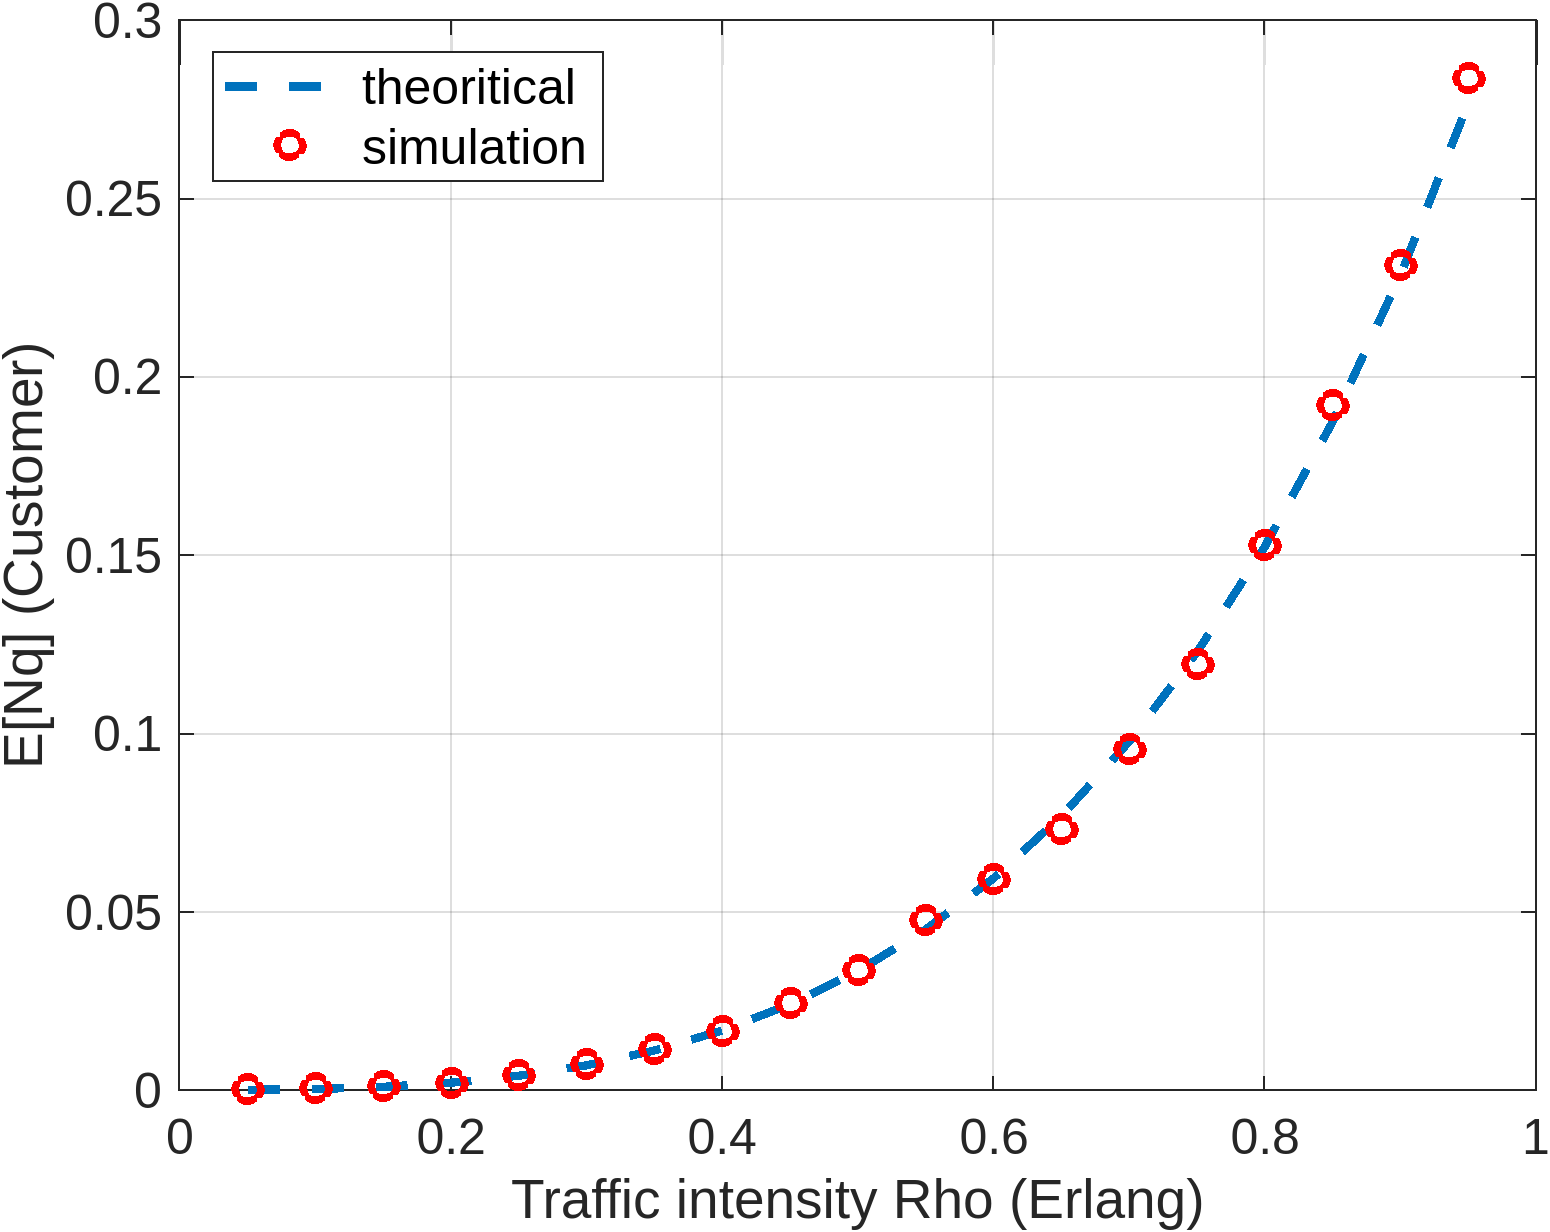
\includegraphics[width=200px]{../code/figures/avgs_vs_traffic_intensity/E_Nq.png}
  } 
  \caption{$E[T], E[W], E[N], \text{and}, E[N_q]$ 
  \\ as function of the traffic intensity (for $c=2$)}
  \label{avg_vs_rho}
\end{figure}

Figure \ref{avg_vs_rho} shows plots for the average total time spent 
in the system $E[T]$, the average waiting time in  the buffer $E[W]$,
the average number of customers in the system $E[N]$, and the average 
number of customers in the buffer $E[N_q]$. All quantities increase as
the traffic intensity increases, which is expected since the increase 
of the traffic intensity implies that the arrival rate to the system is 
getting relatively larger to the overall service rate of the system. This means 
that the system is becoming more saturated and hence the averages for 
the total time, the waiting time, and the total number of customers
in the system and in the buffer increase. Furthermore, Figure \ref{avg_vs_rho} 
shows that the simulation results agree with the theoretical ones.

\subsection{PDF of the total time}
\begin{figure}[H]
  \centering
  \subfloat[]{
    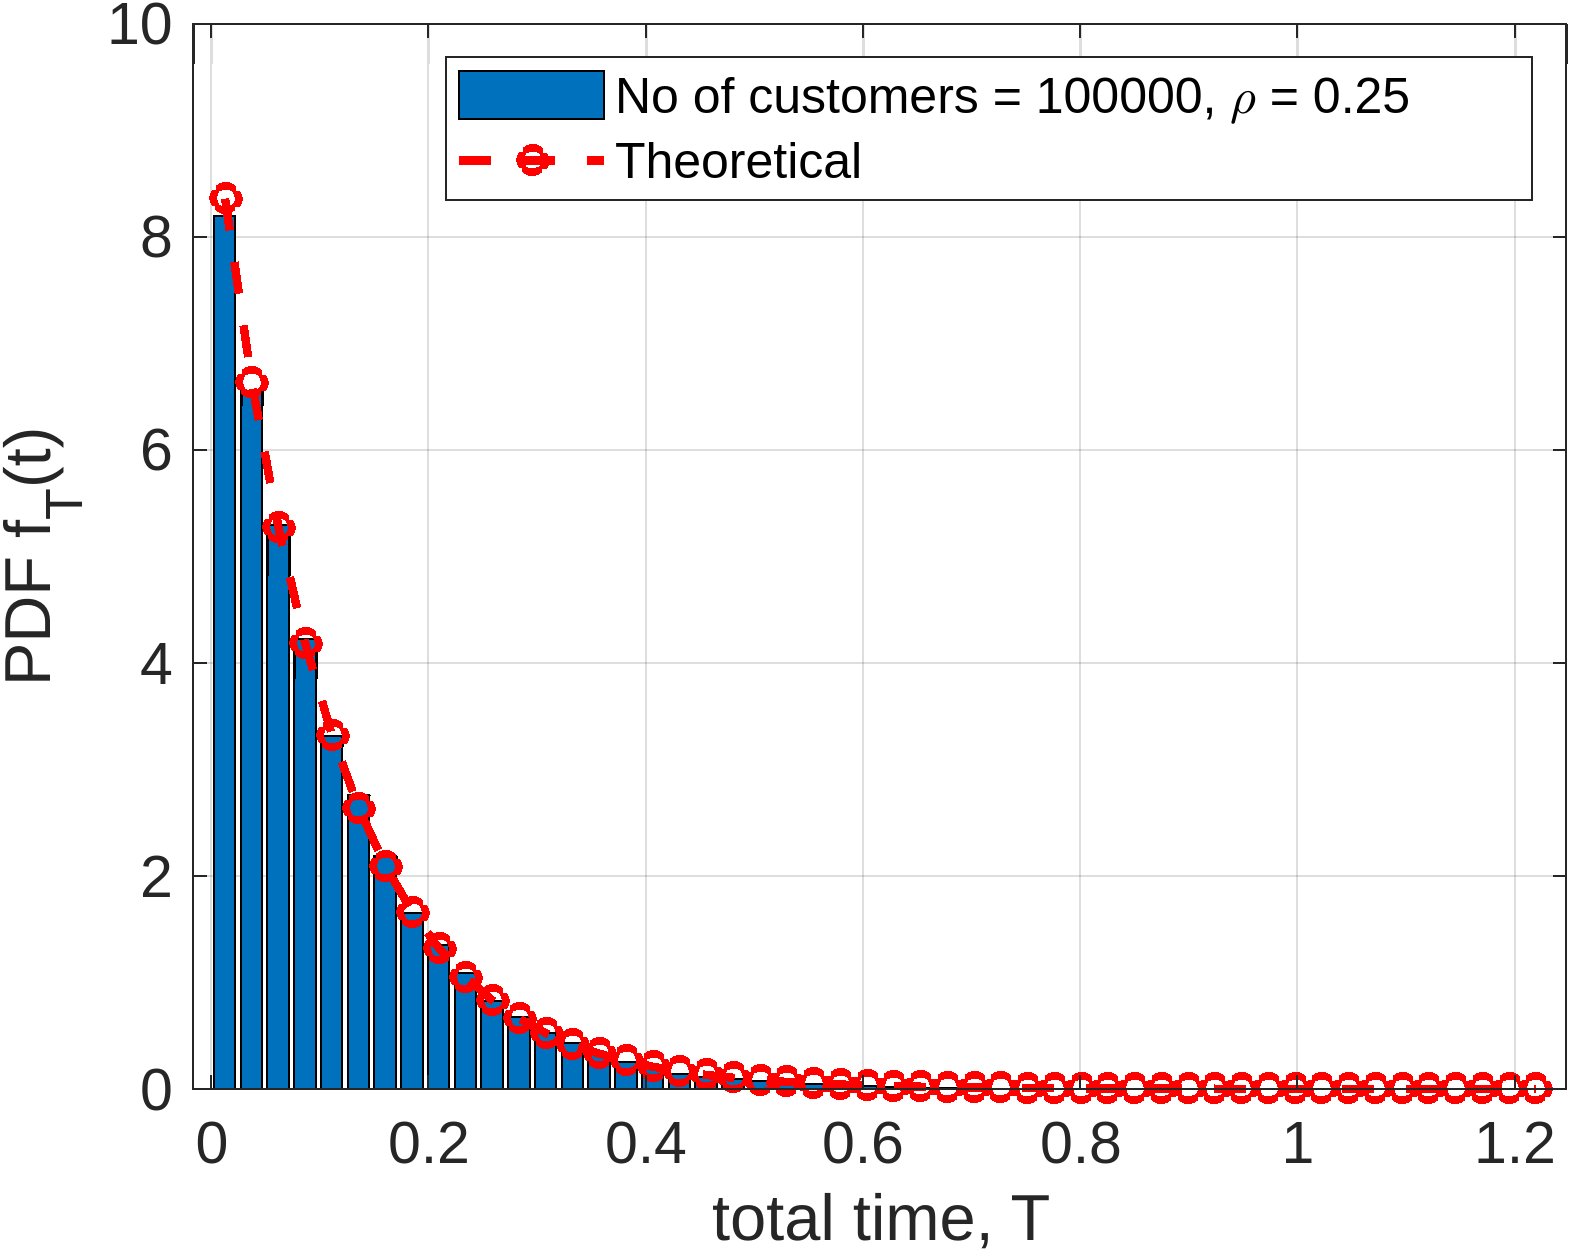
\includegraphics[width=200px]{../code/figures/total_time_dist/bars_plot_no_customers_100000_rho_0.25.png}
  }
  \subfloat[]{
    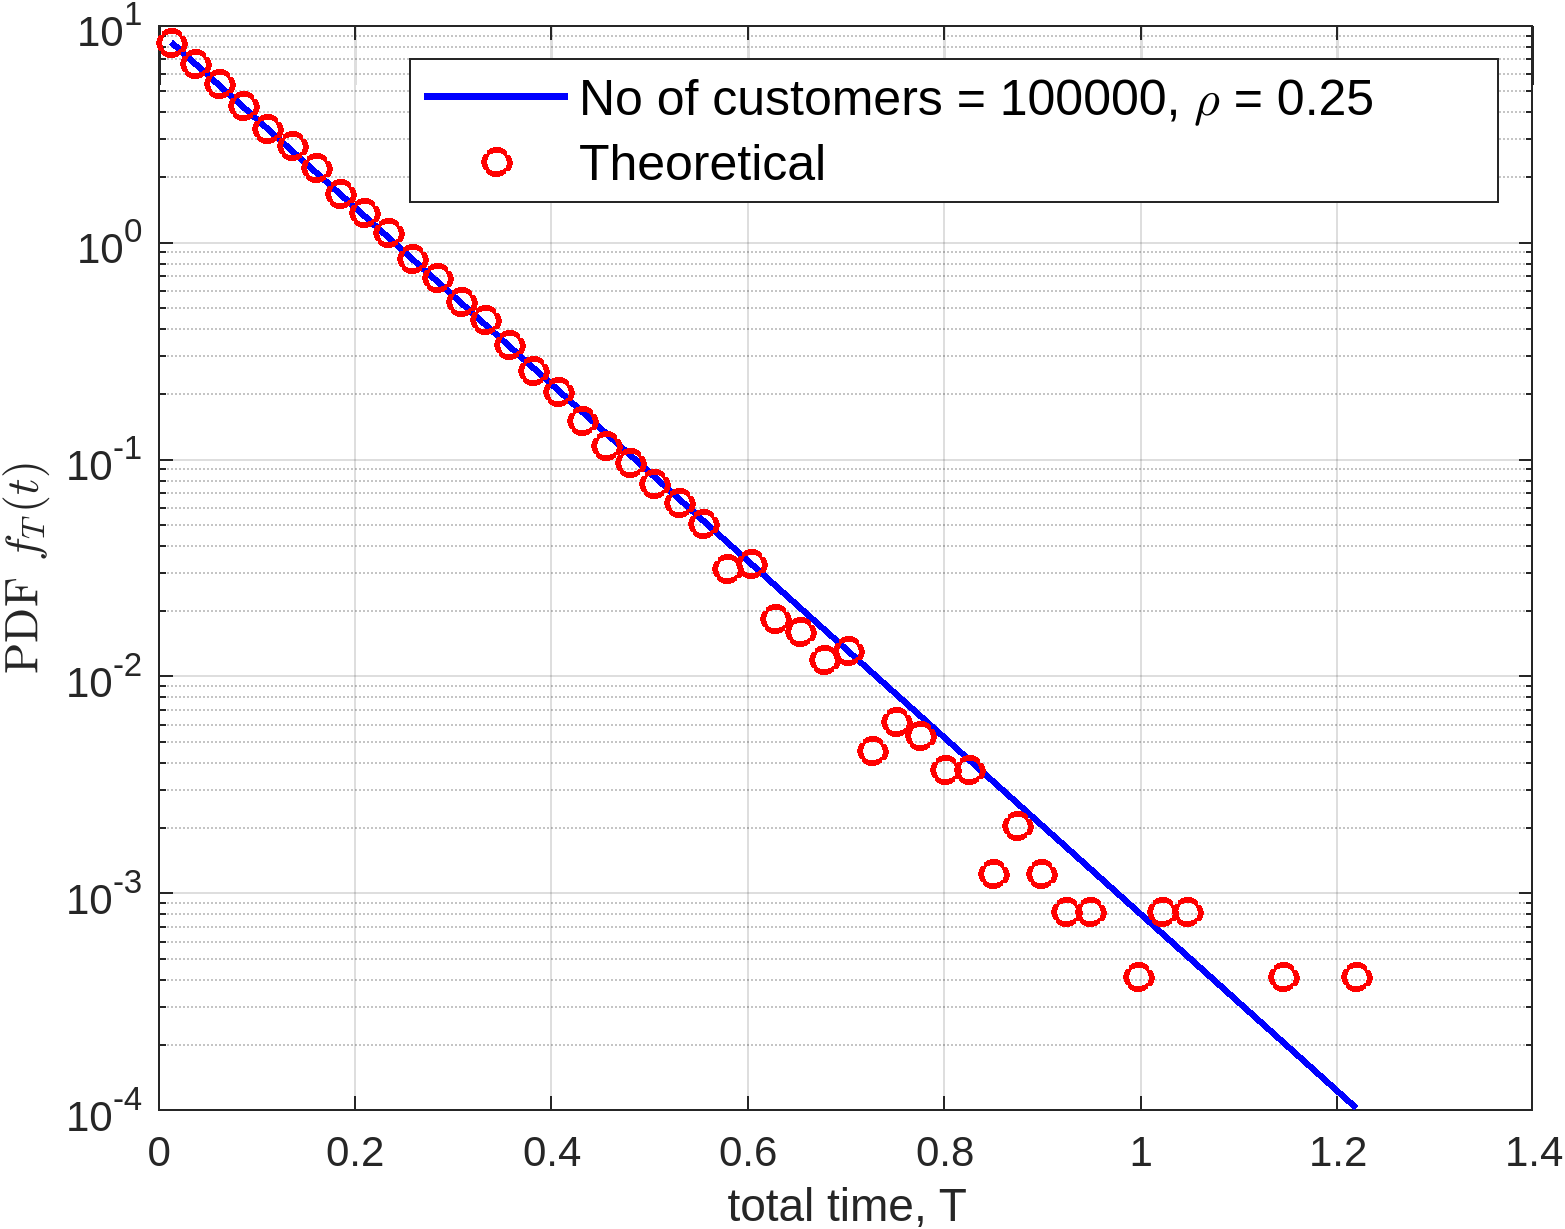
\includegraphics[width=200px]{../code/figures/total_time_dist/semilogy_plot_no_customers_100000_rho_0.25.png}
  }
  \hspace{0px}
  \subfloat[]{
    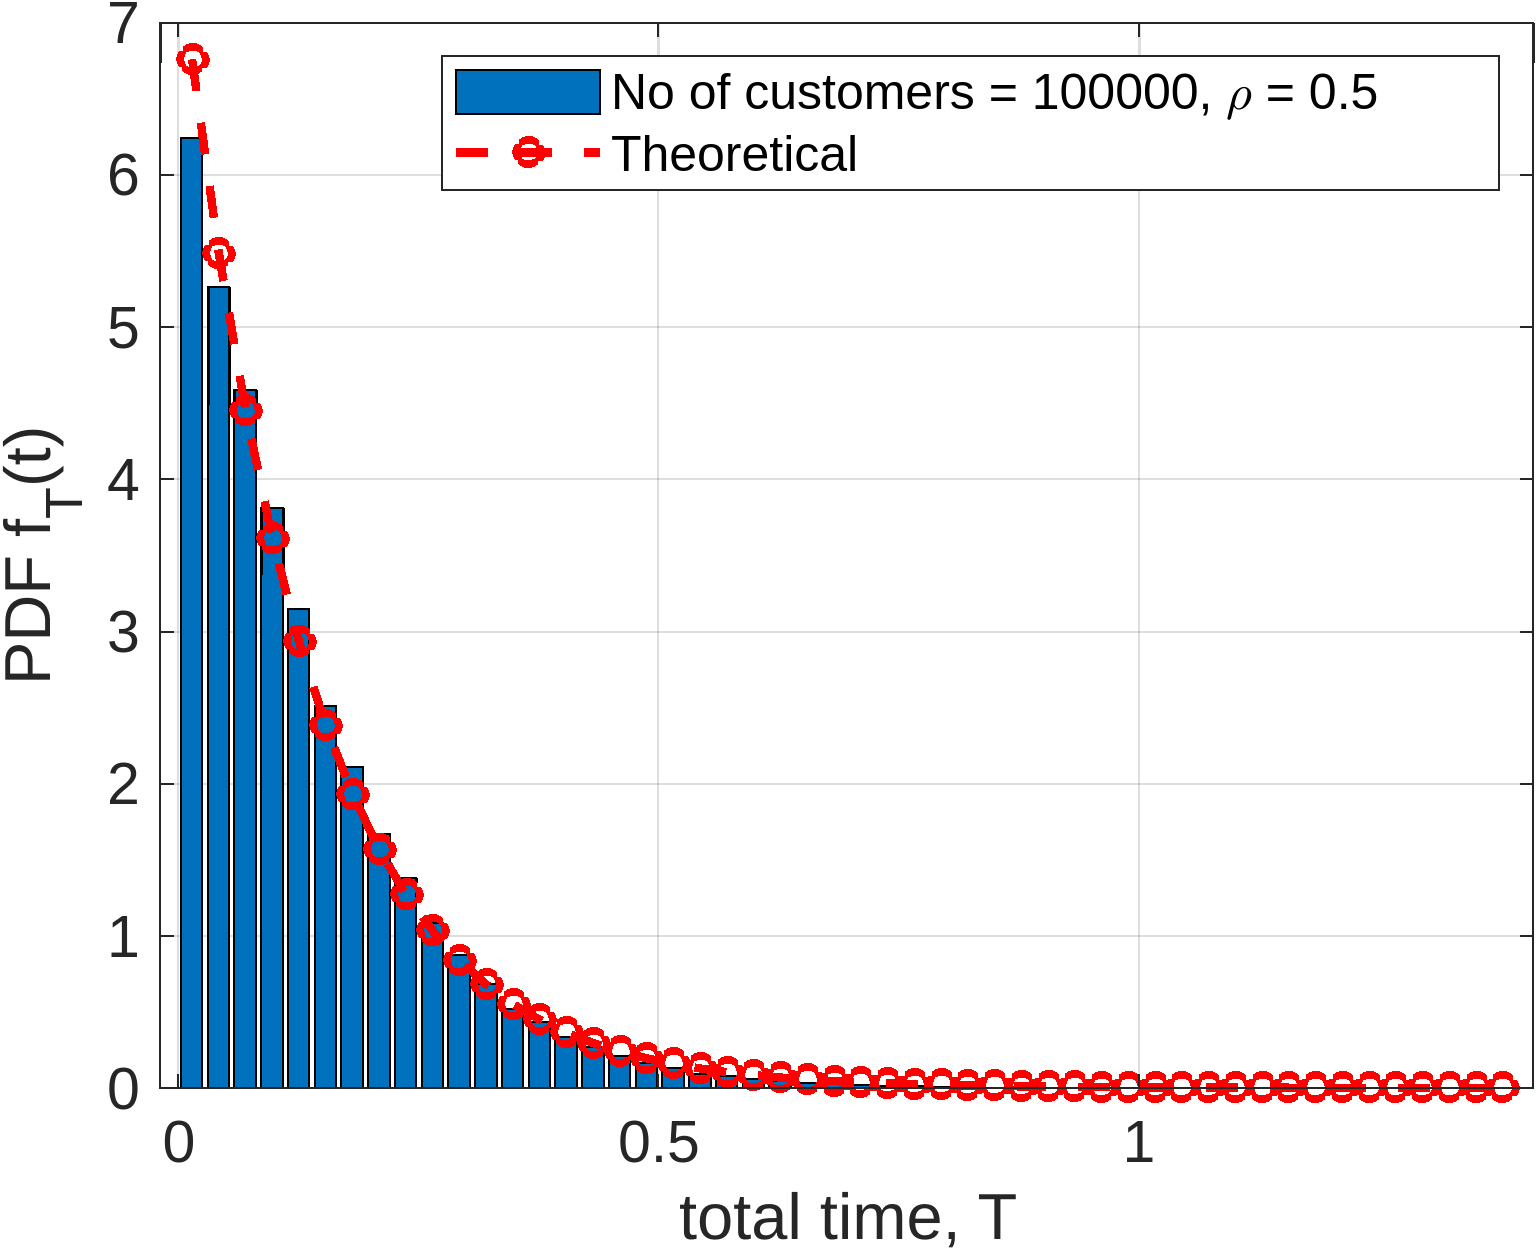
\includegraphics[width=200px]{../code/figures/total_time_dist/bars_plot_no_customers_100000_rho_0.5.png}
  }
  \subfloat[]{
    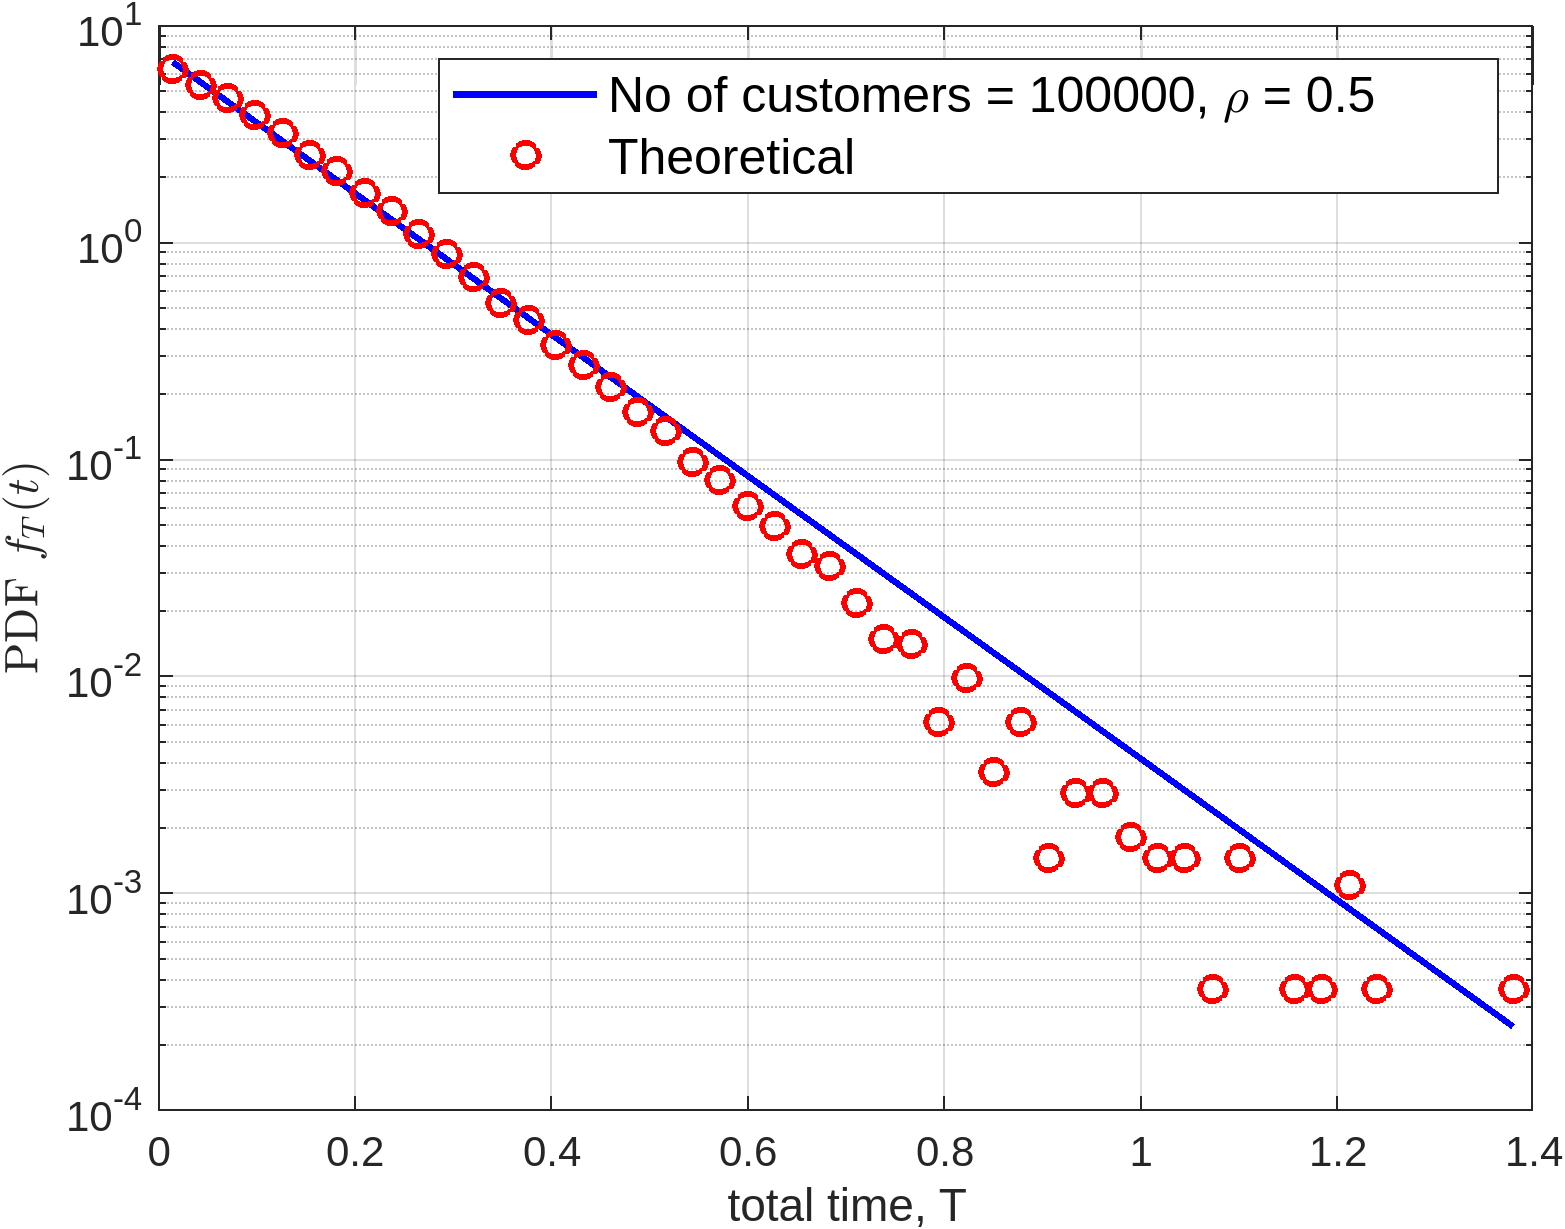
\includegraphics[width=200px]{../code/figures/total_time_dist/semilogy_plot_no_customers_100000_rho_0.5.png}
  }
  \caption{PDF of the total time in the system for low and medium traffic intensity}
  \label{PDF_TT_low_med}
\end{figure}

\begin{figure}[H]
  \centering
  \subfloat[]{
    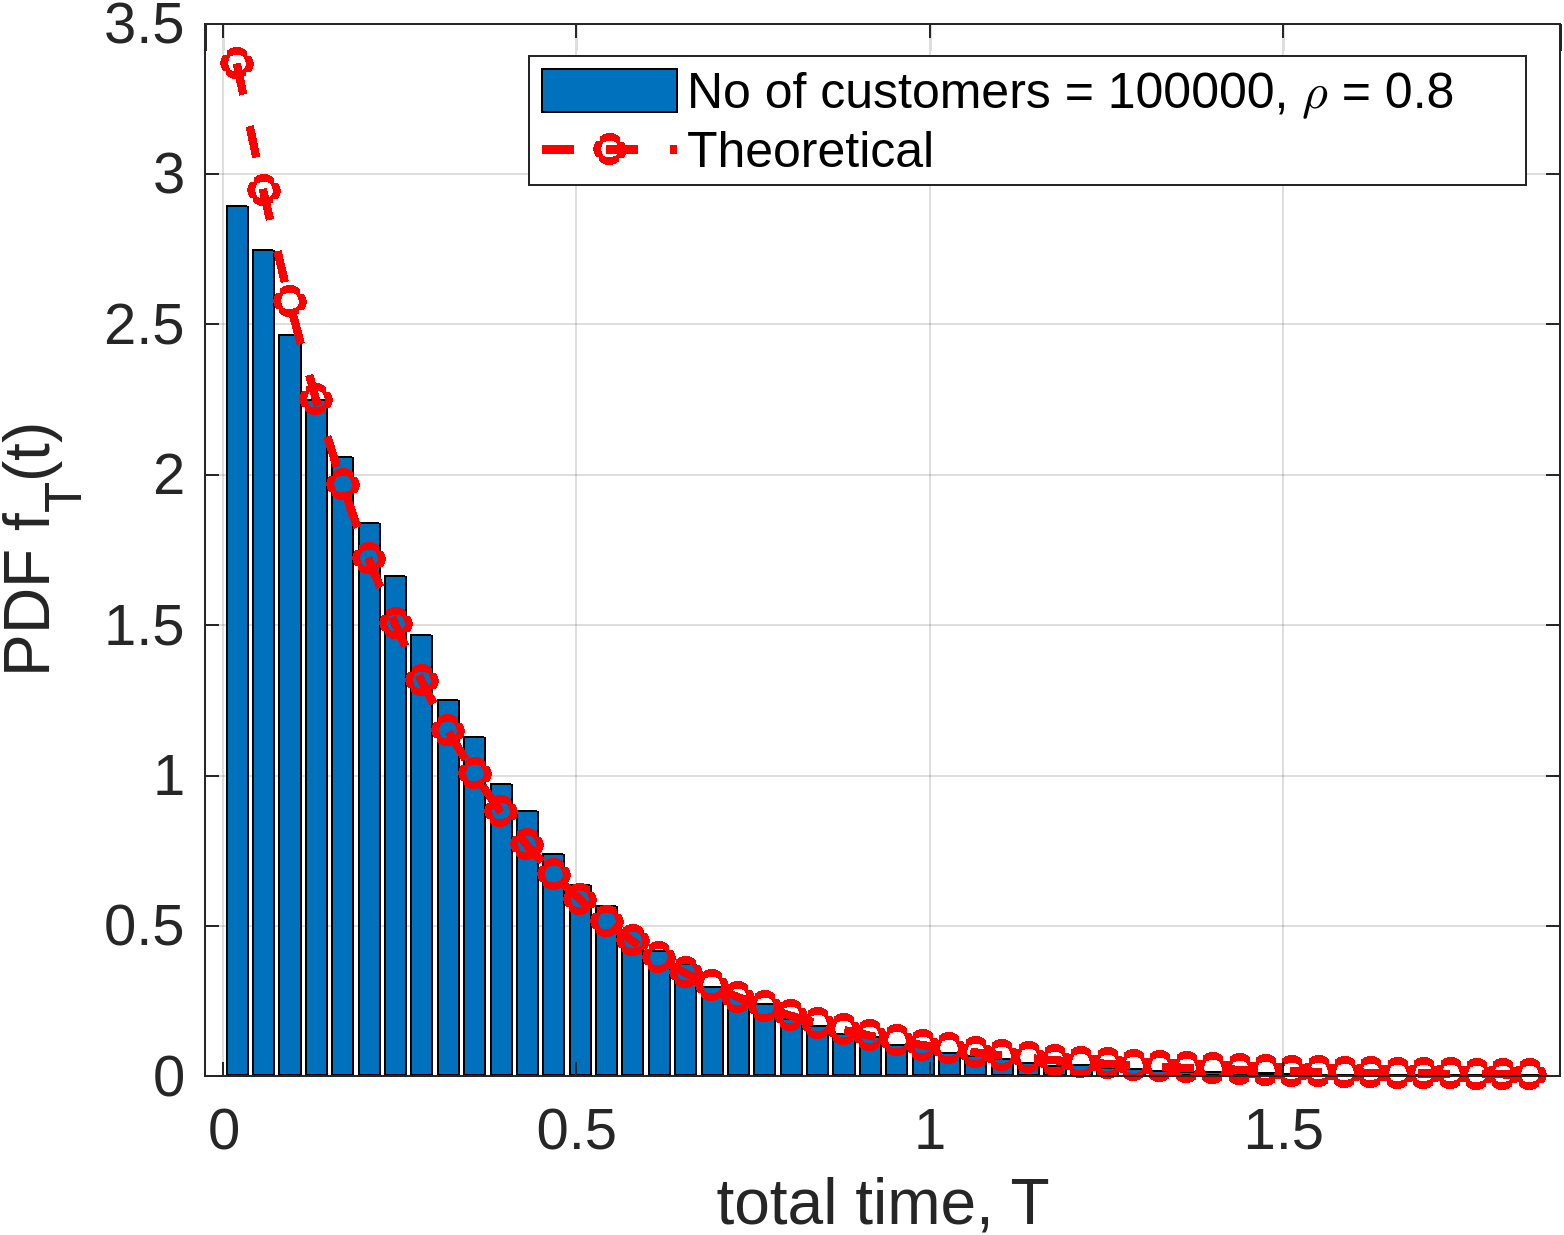
\includegraphics[width=200px]{../code/figures/total_time_dist/bars_plot_no_customers_100000_rho_0.8.png}
  }
  \subfloat[]{
    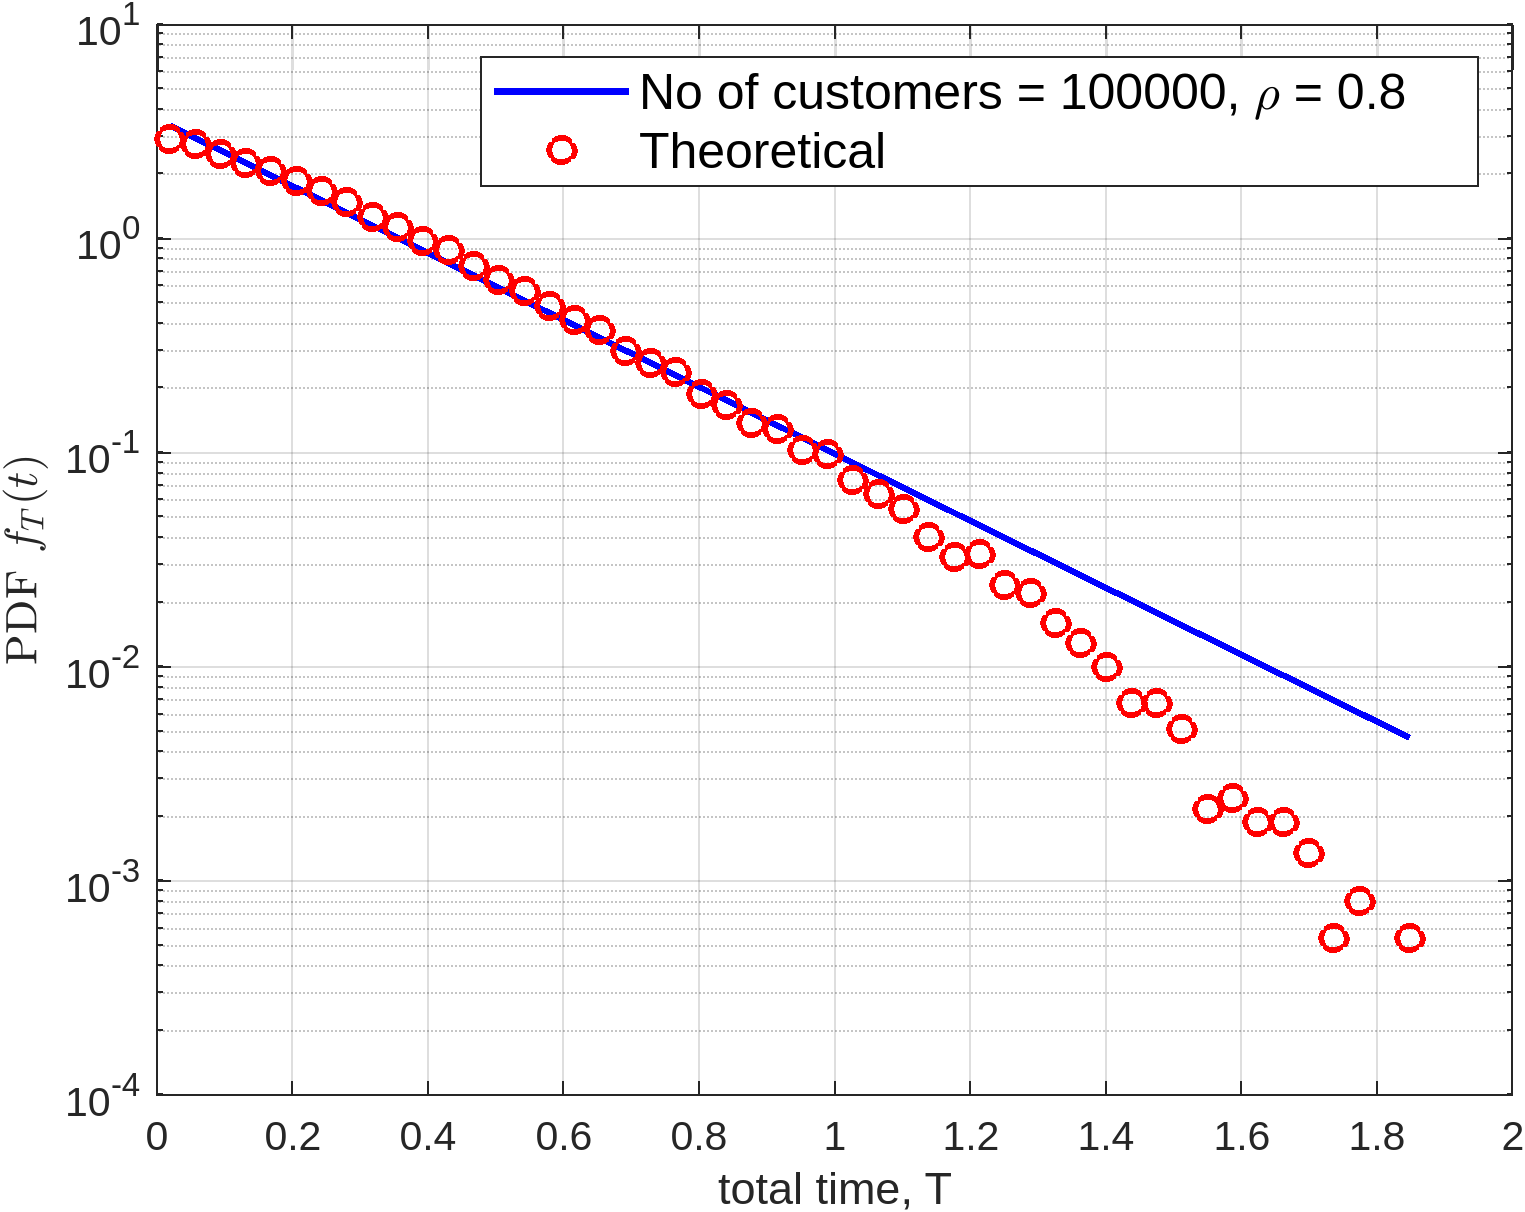
\includegraphics[width=200px]{../code/figures/total_time_dist/semilogy_plot_no_customers_100000_rho_0.8.png}
  }
  \hspace{0px}
  \subfloat[]{
    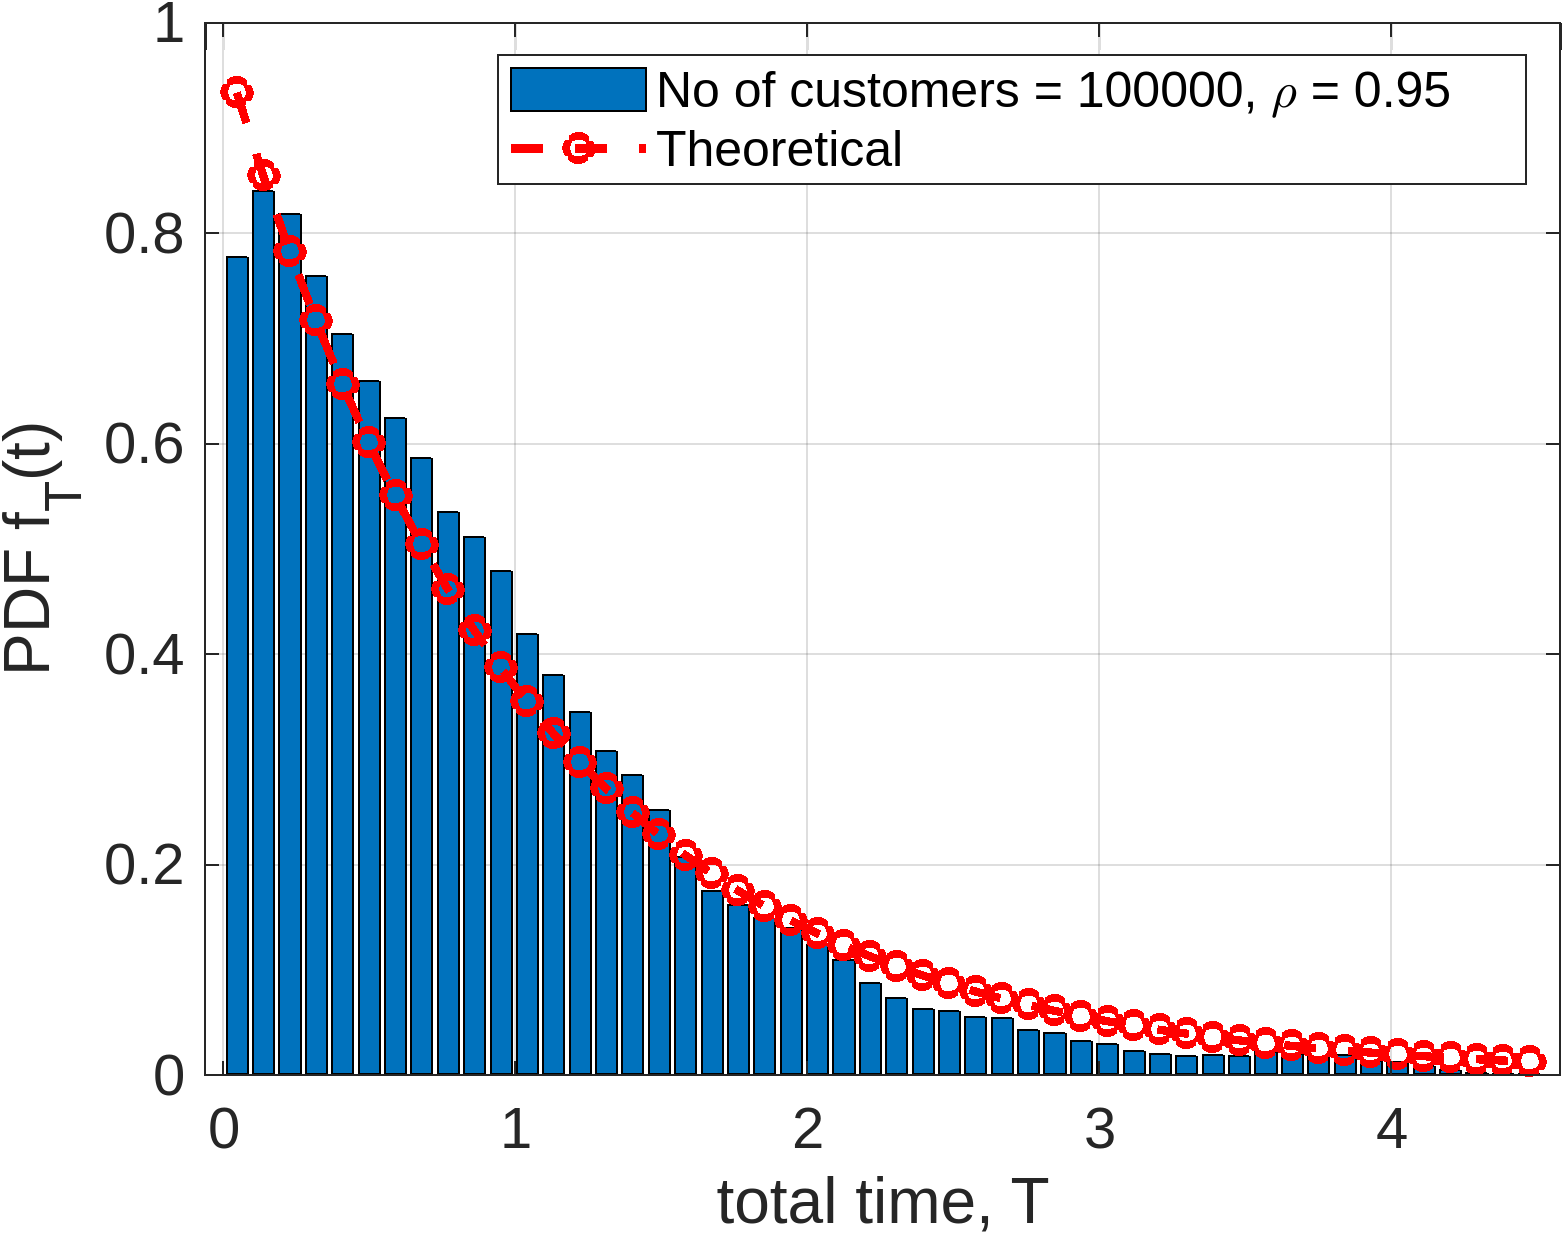
\includegraphics[width=200px]{../code/figures/total_time_dist/bars_plot_no_customers_100000_rho_0.95.png}
  }
  \subfloat[]{
    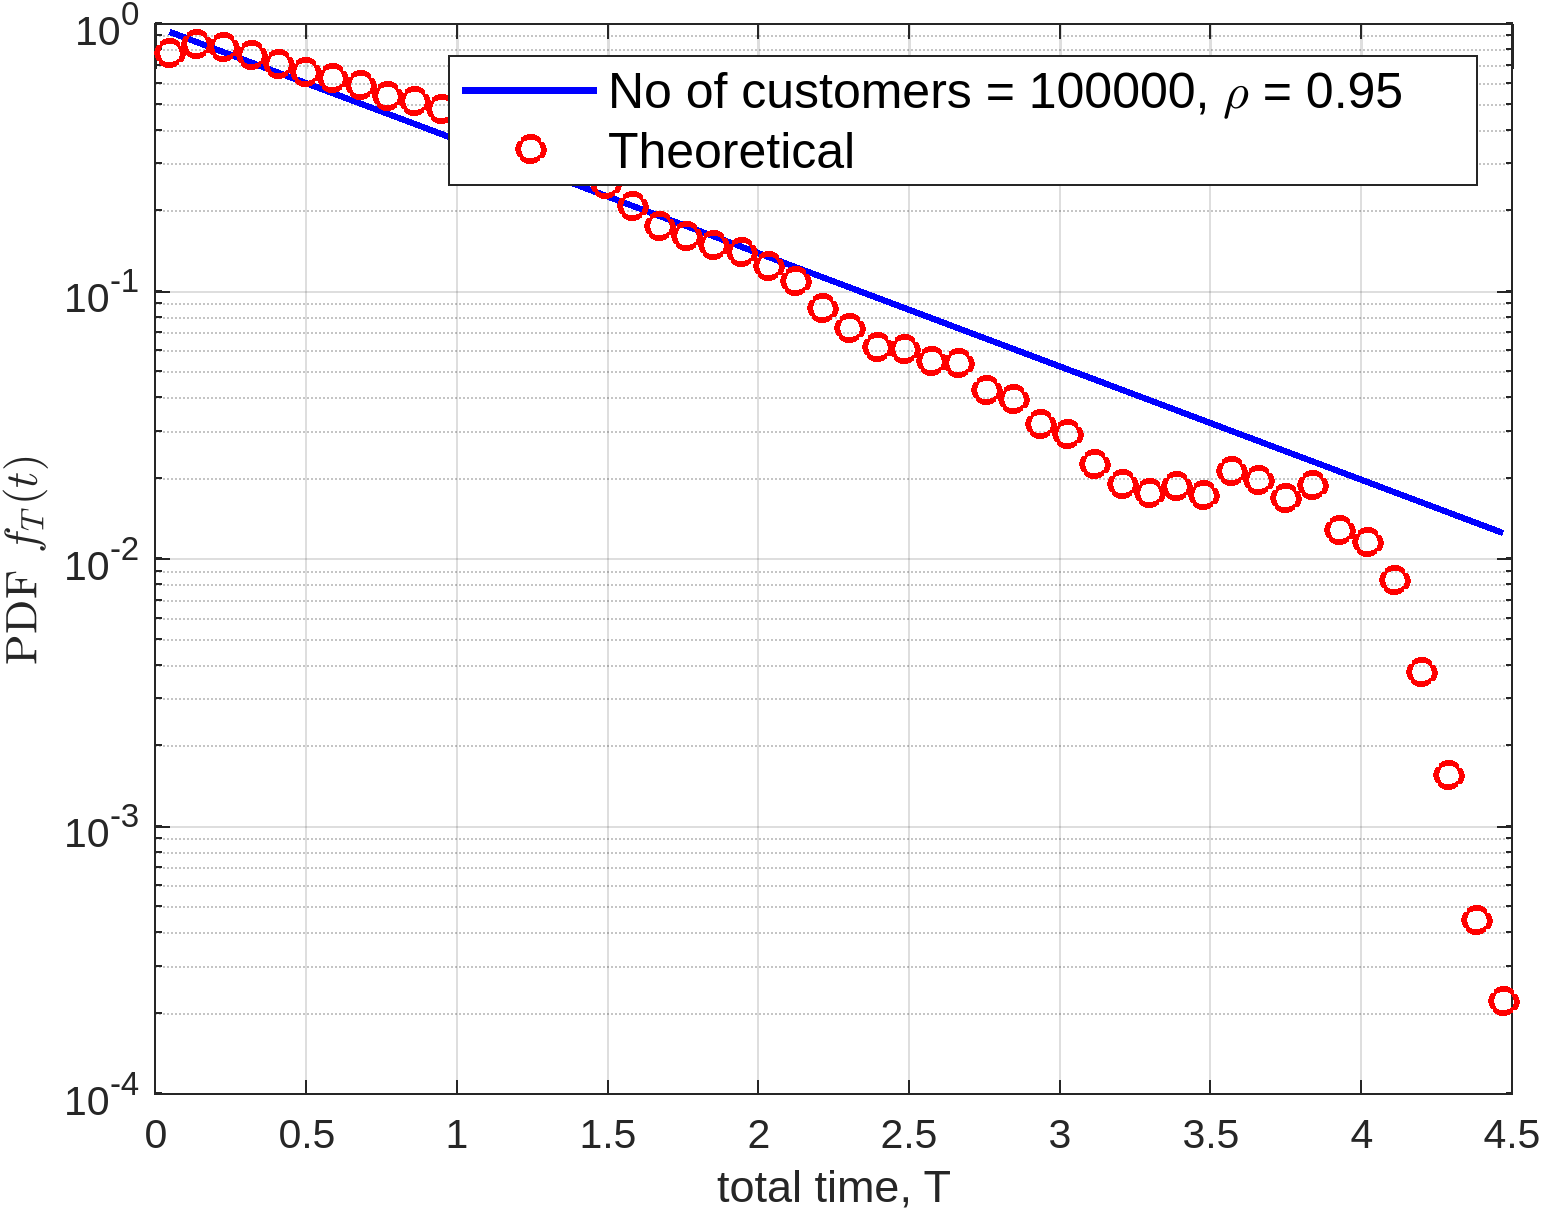
\includegraphics[width=200px]{../code/figures/total_time_dist/semilogy_plot_no_customers_100000_rho_0.95.png}
  }
  \caption{PDF of the total time in the system for high traffic intensity}
  \label{PDF_TT_high}
\end{figure}

Figure \ref{PDF_TT_low_med} shows the probability density function (PDF) 
for the total time spent in the system for a low traffic intensity, $\rho = 0.25$
and a medium traffic intensity, $\rho=0.5$. The distribution is exponential as expected
from the theoretical formula. Moreover, the empirical and the theoretical distribution
are in an excellent agreement.

Figure \ref{PDF_TT_high} shows the PDF for the total time for high traffic intensities, 
$\rho=0.8$ and $\rho=0.95$. They agree with the theoretical ones, but not as well as 
in the case low and medium traffic intensities. In an attempt to resolve this issue,
we increased the number of customers to $1000000$ as indicated in Figure \ref{PDF_TT_high_more_cus}.
This resulted in a better agreement with the theoretical results.

\begin{figure}[H]
  \centering
  \subfloat[]{
    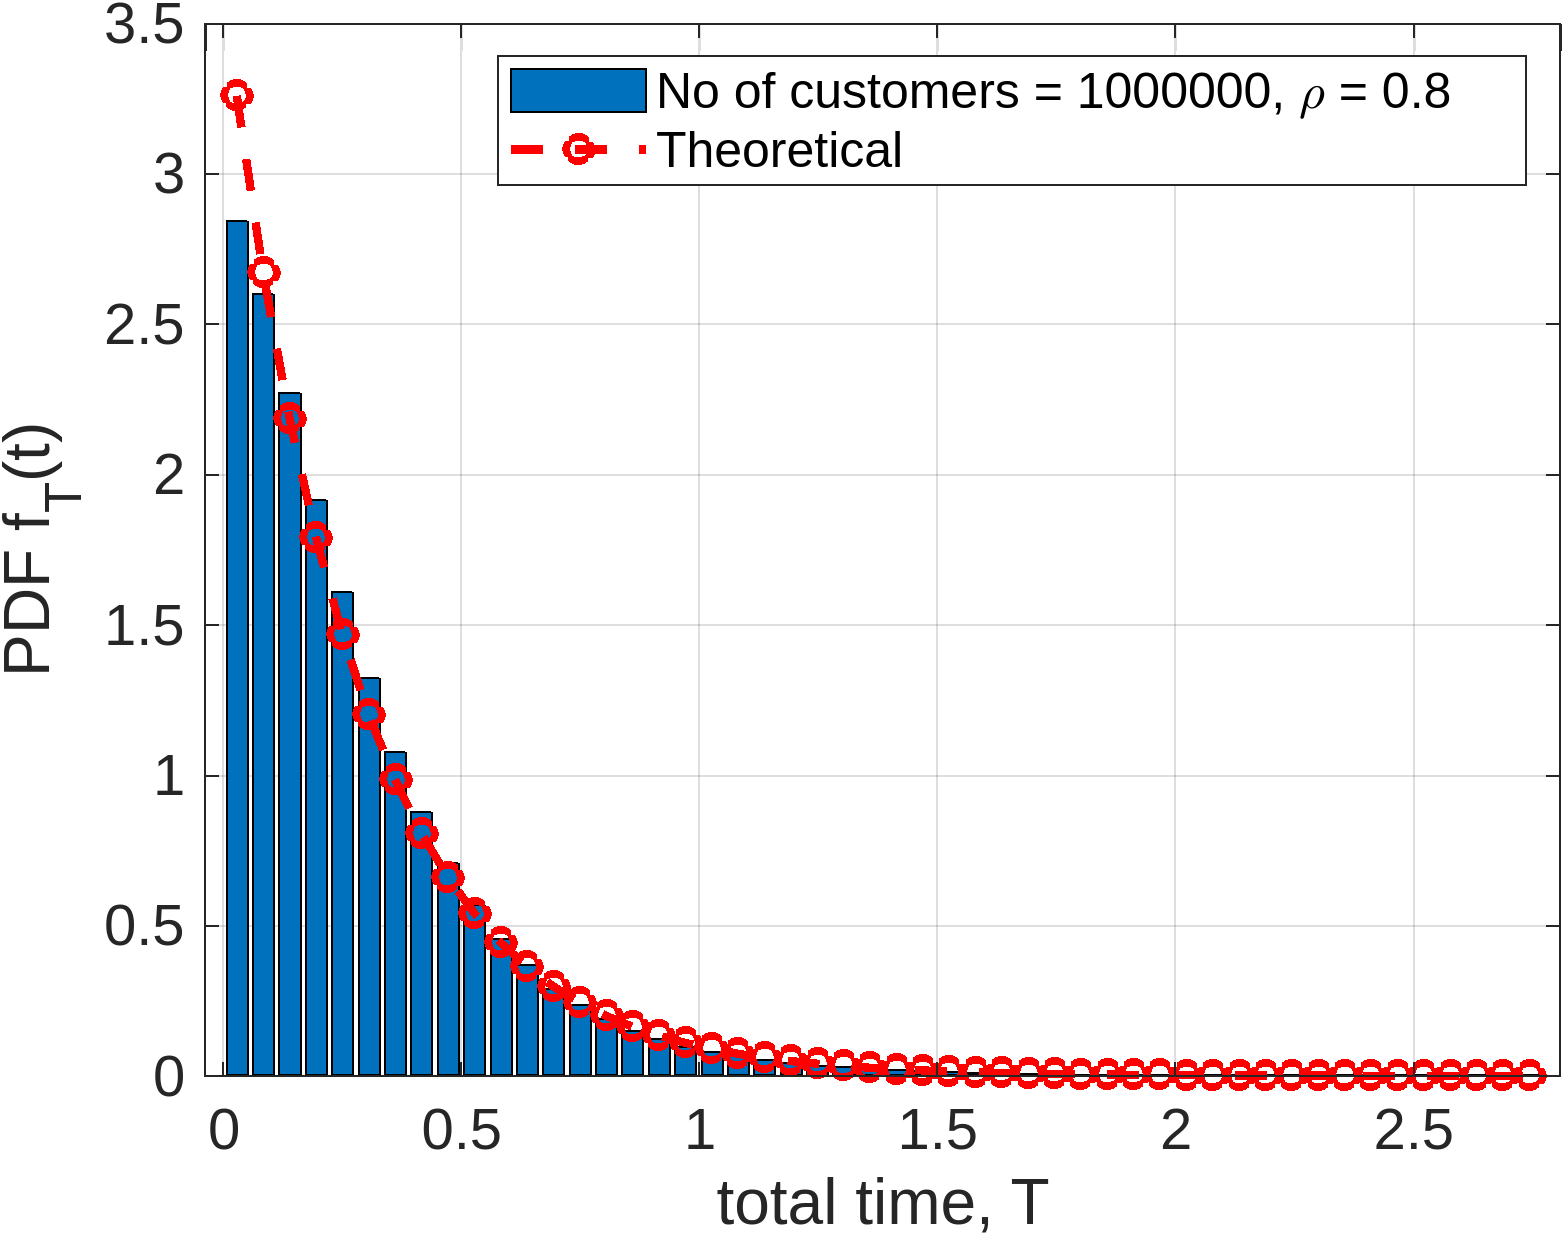
\includegraphics[width=200px]{../code/figures/total_time_dist/bars_plot_no_customers_1000000_rho_0.8.png}
  }
  \subfloat[]{
    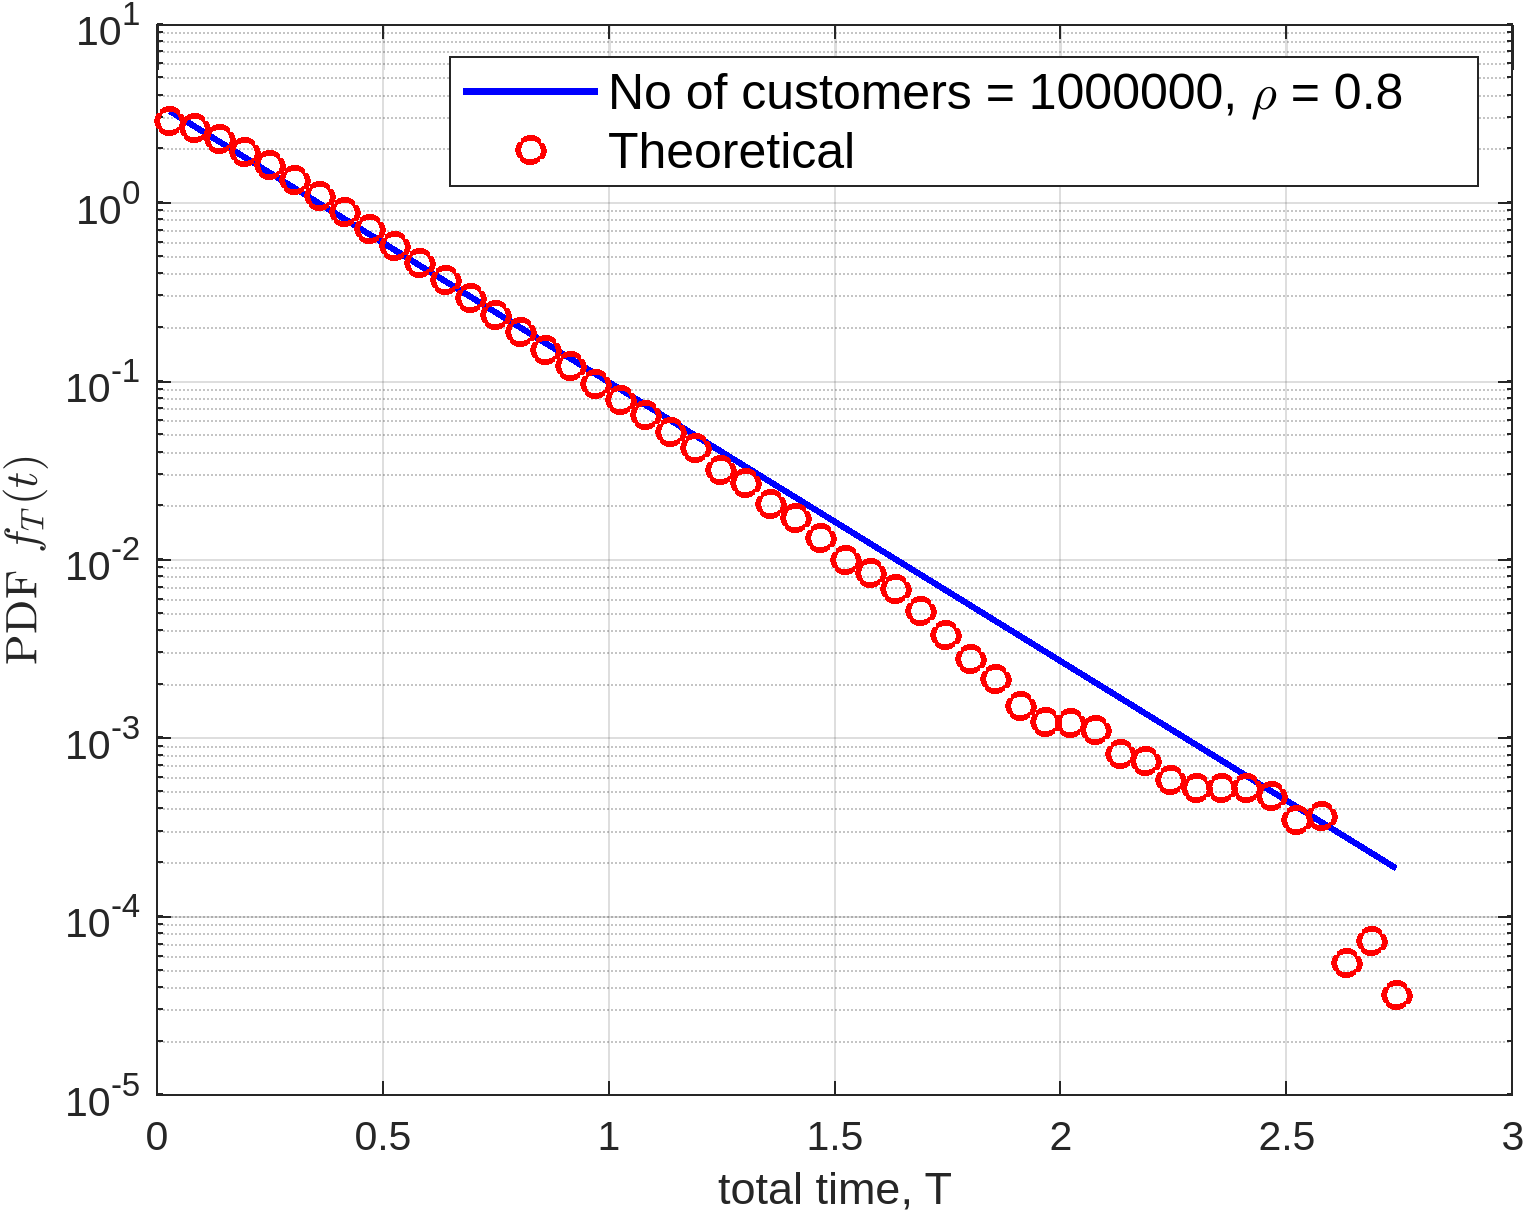
\includegraphics[width=200px]{../code/figures/total_time_dist/semilogy_plot_no_customers_1000000_rho_0.8.png}
  }
  \hspace{0px}
  \subfloat[]{
    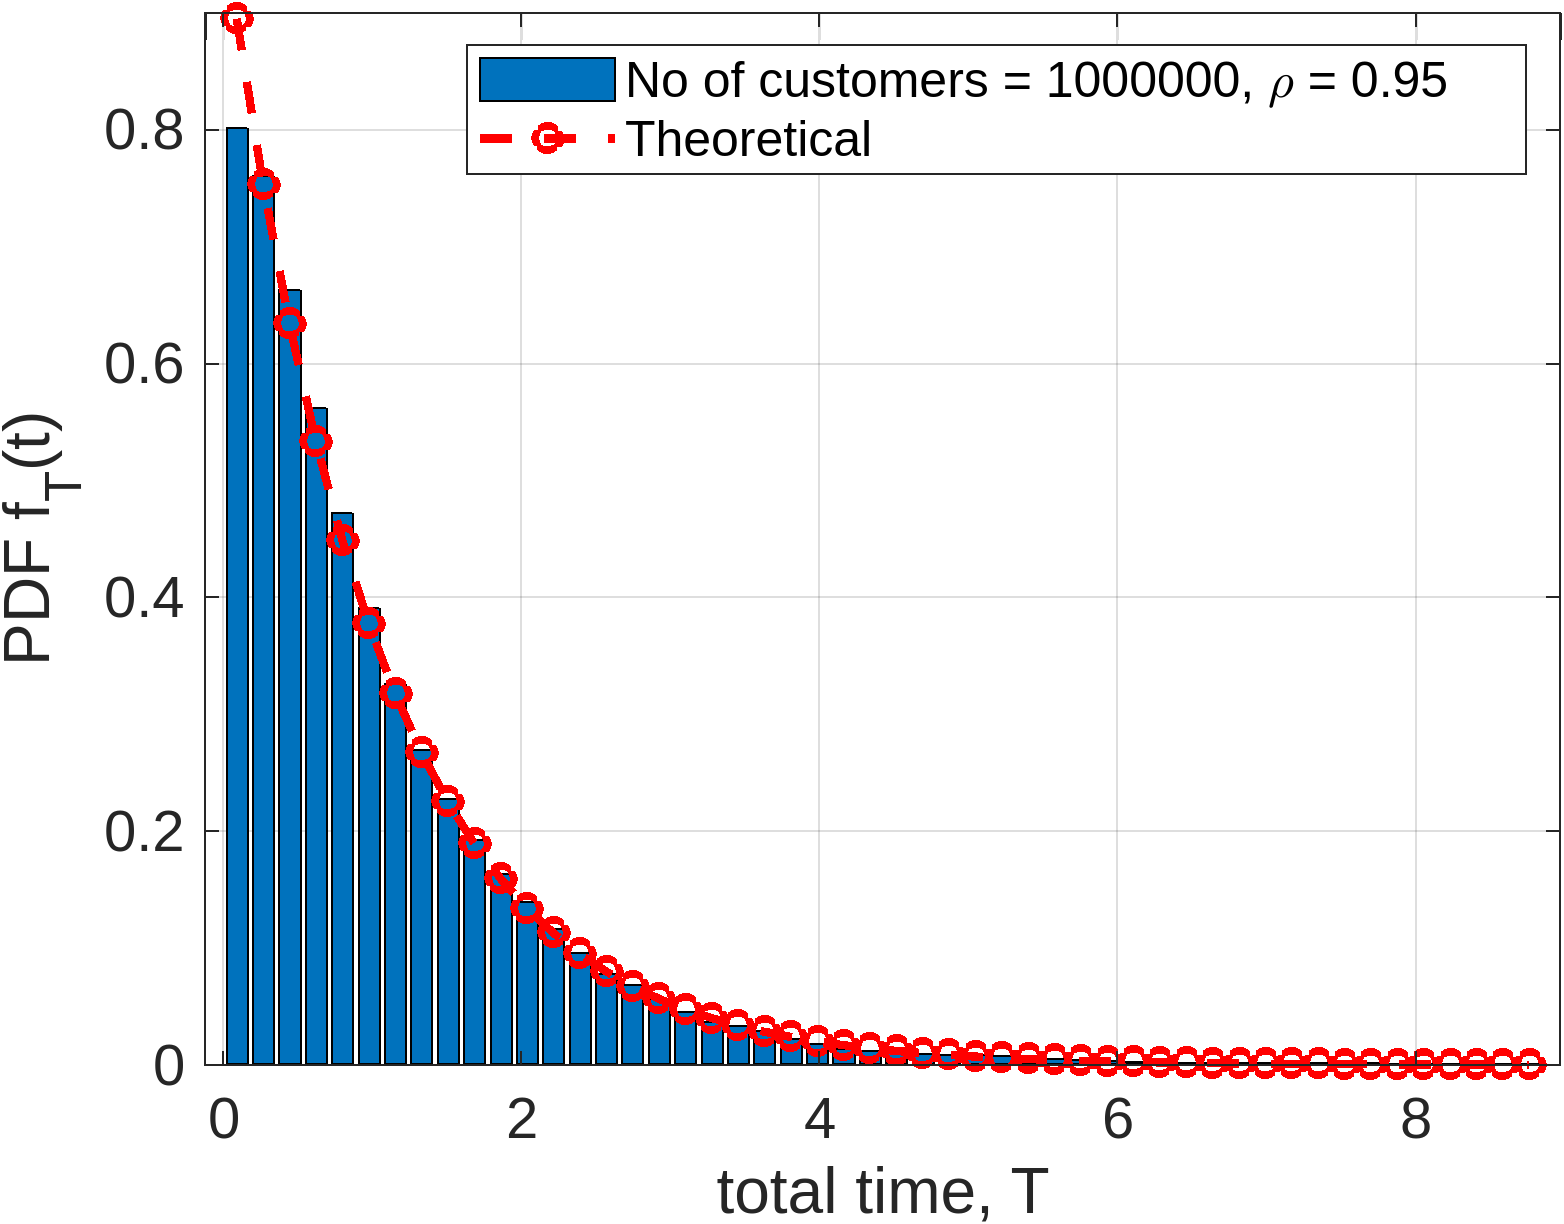
\includegraphics[width=200px]{../code/figures/total_time_dist/bars_plot_no_customers_1000000_rho_0.95.png}
  }
  \subfloat[]{
    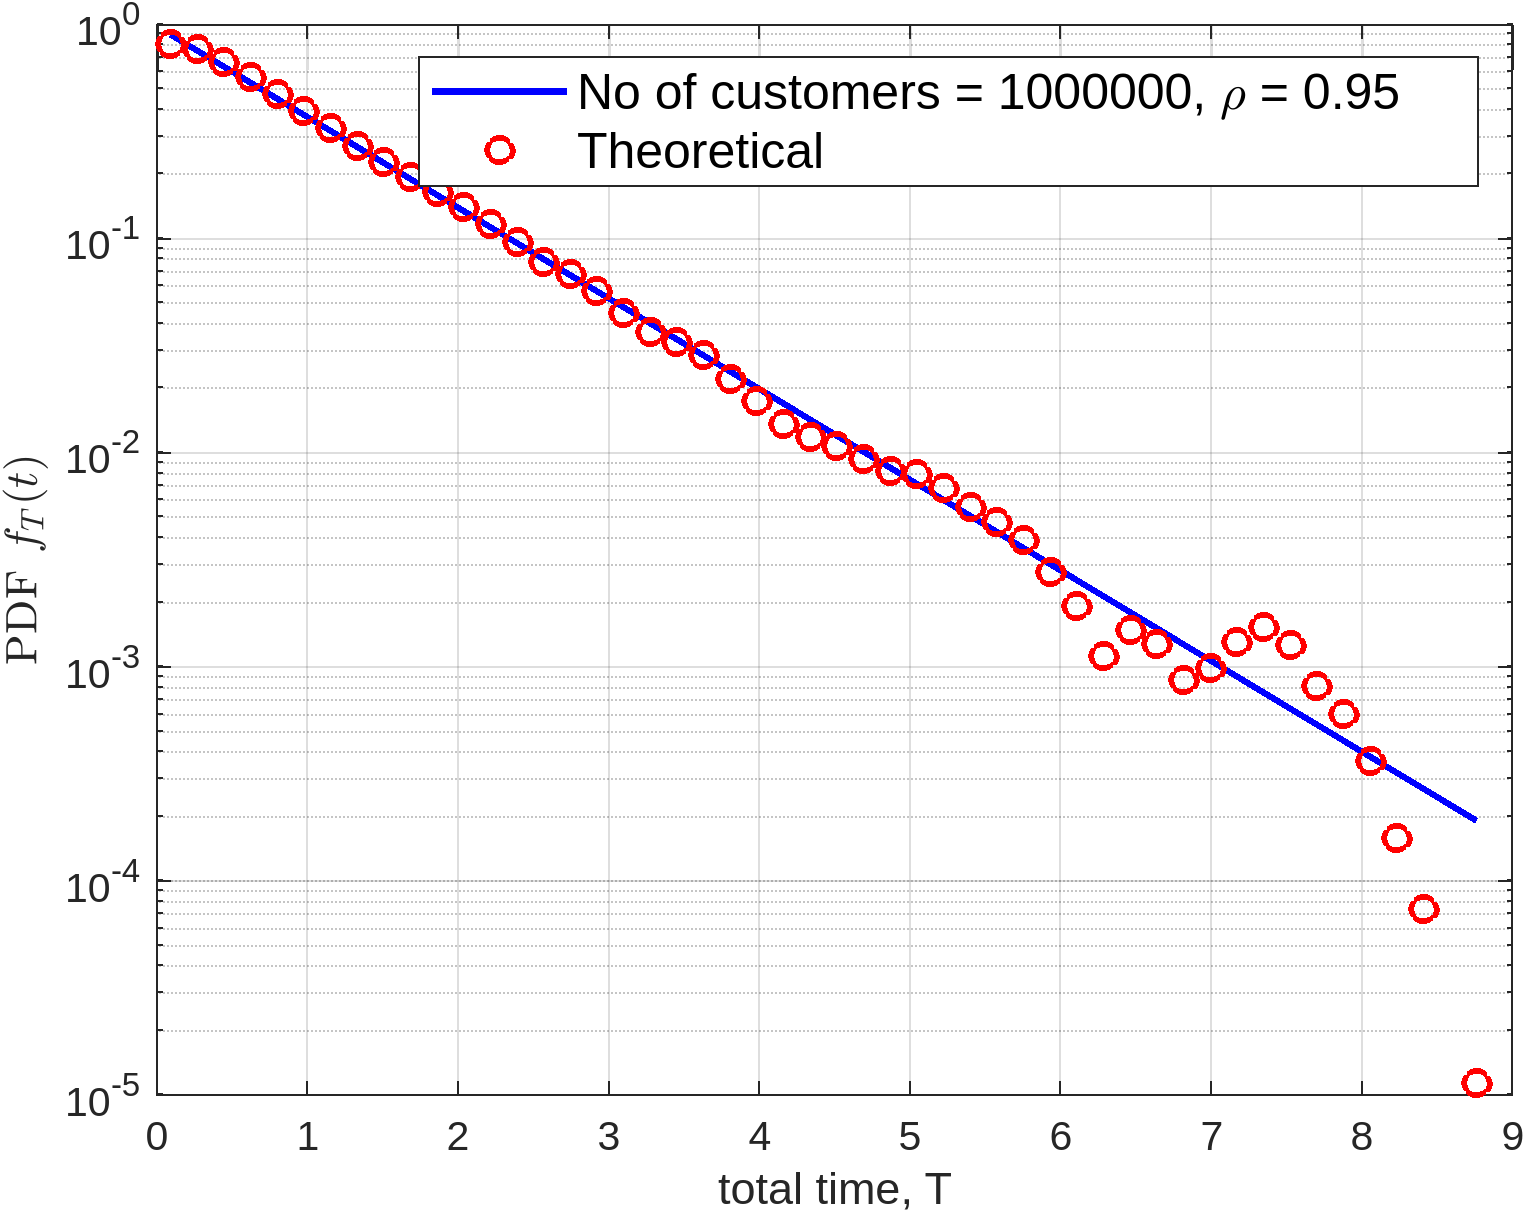
\includegraphics[width=200px]{../code/figures/total_time_dist/semilogy_plot_no_customers_1000000_rho_0.95.png}
  }
  \caption{PDF of the total time in the system for high $\rho$ and $1000000$ customers}  
  \label{PDF_TT_high_more_cus}
\end{figure}

\subsection{PDF of the waiting time}
\begin{figure}[H]
  \centering
  \subfloat[]{
    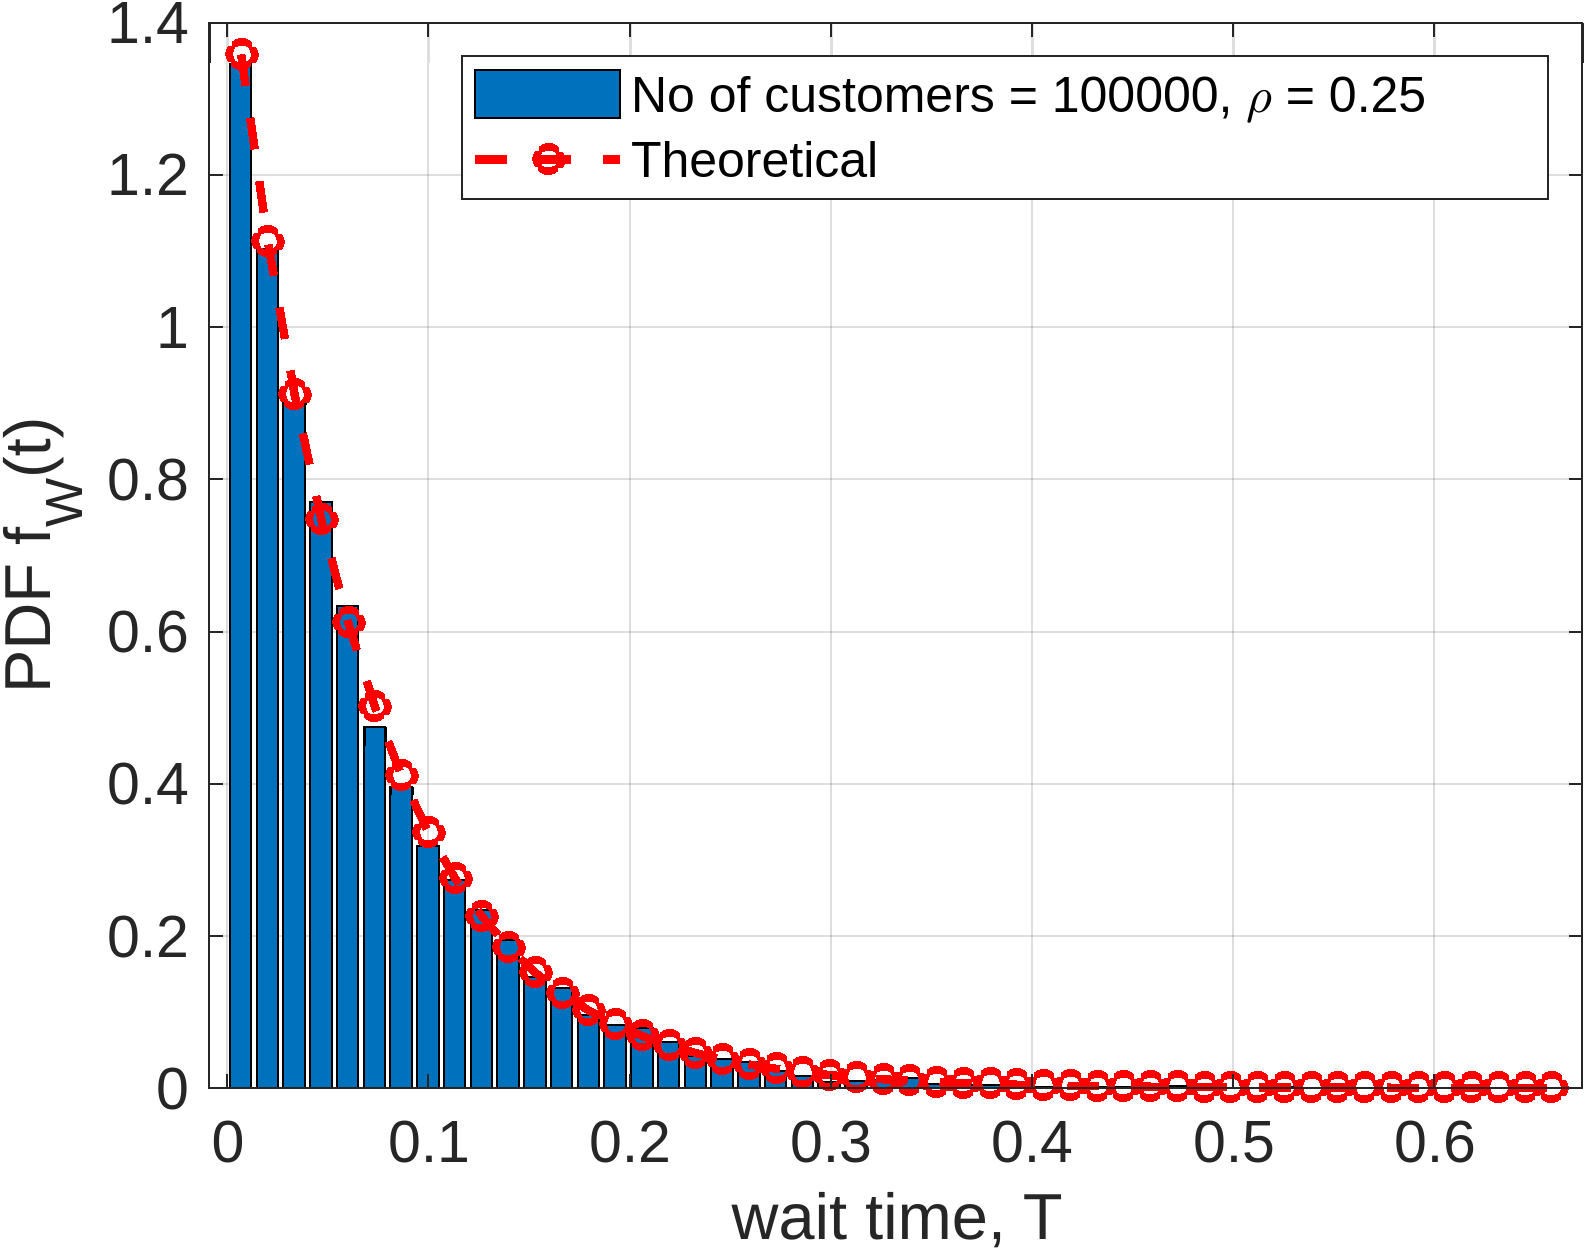
\includegraphics[width=200px]{../code/figures/waiting_time_dist/bar_plot_no_customers_100000_rho_0.25.png}
  }
  \subfloat[]{
    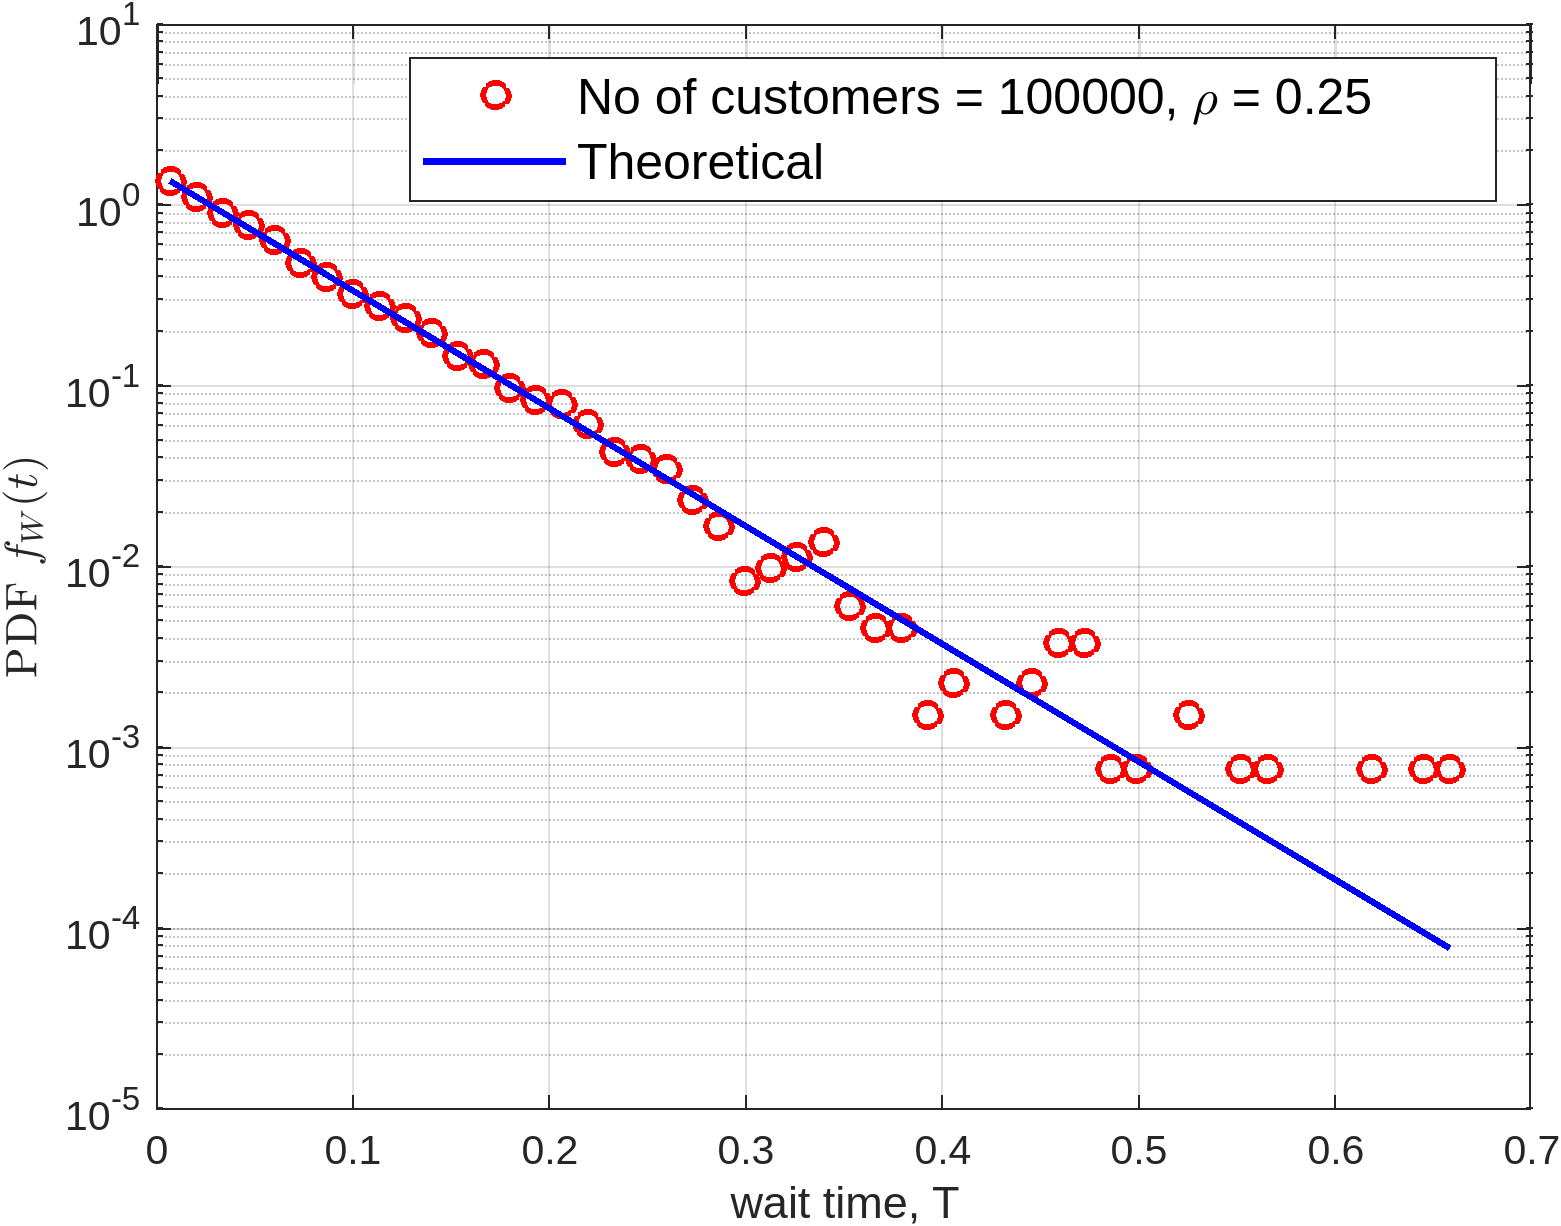
\includegraphics[width=200px]{../code/figures/waiting_time_dist/semilogy_plot_no_customers_100000_rho_0.25.png}
  }
  \hspace{0px}
  \subfloat[]{
    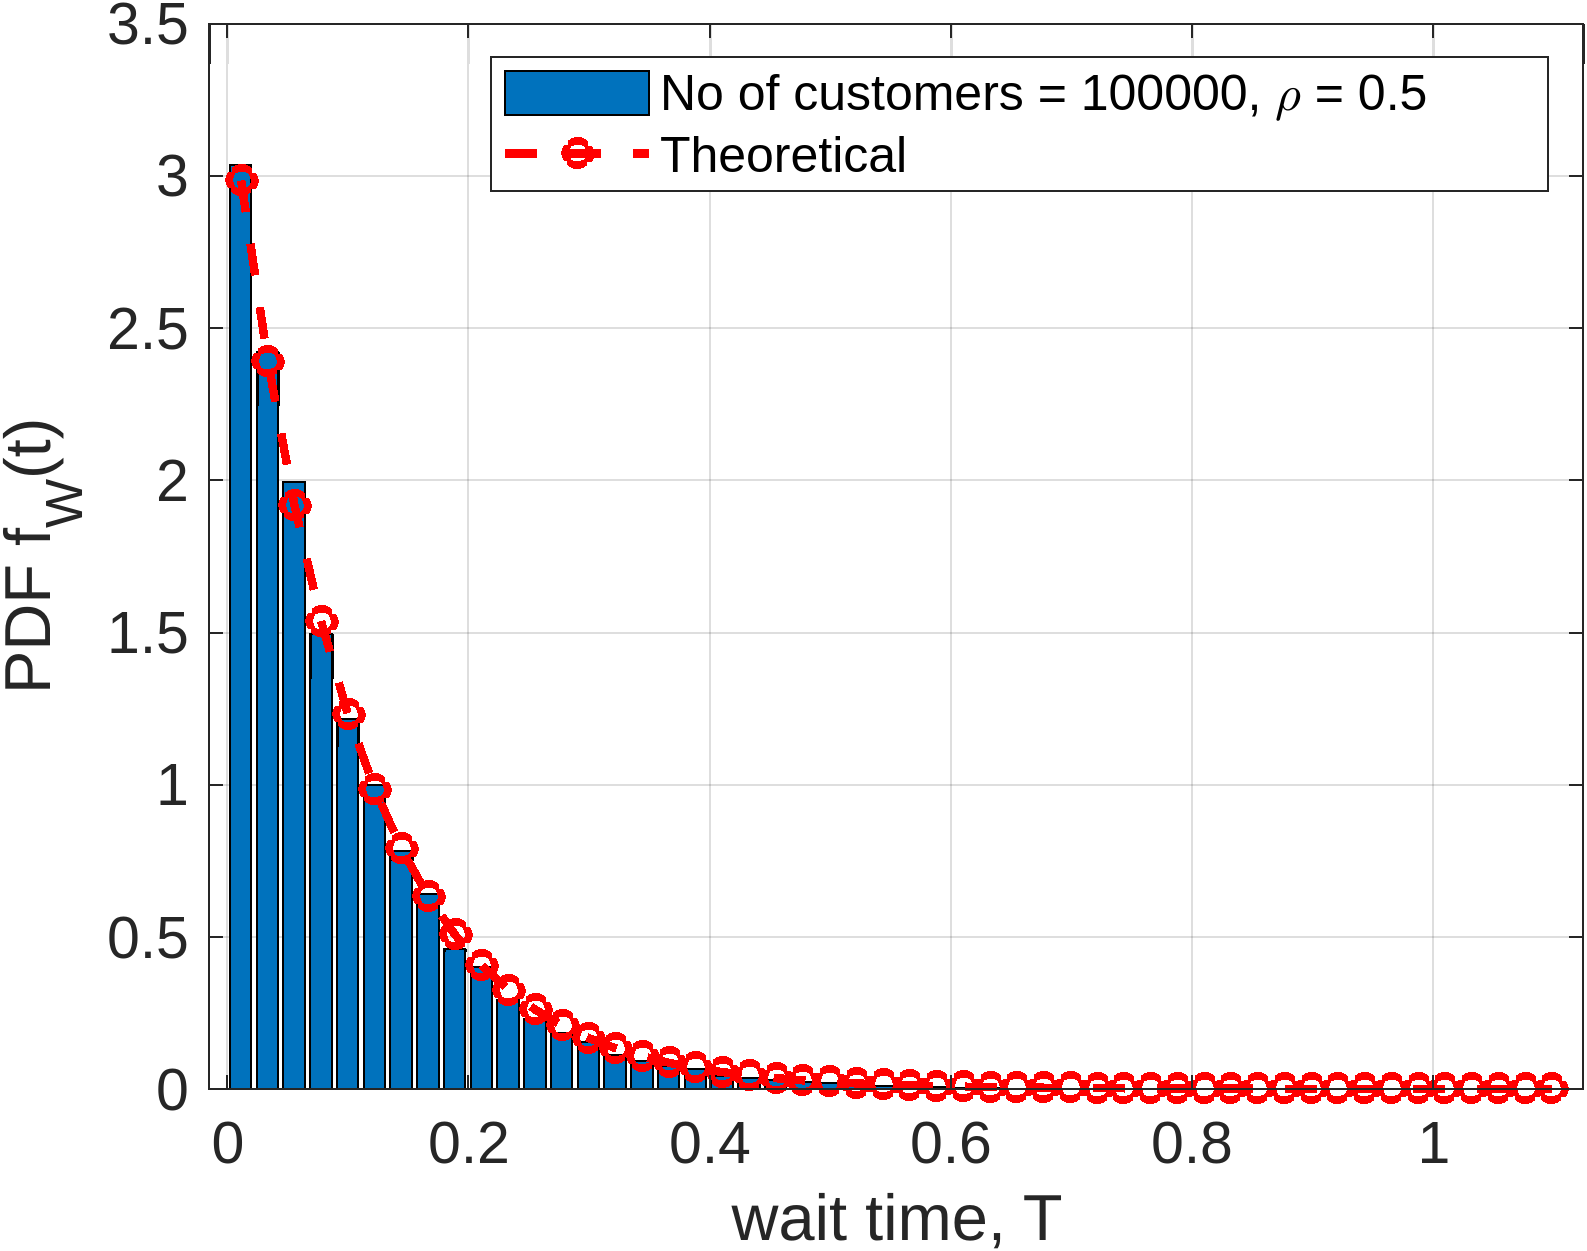
\includegraphics[width=200px]{../code/figures/waiting_time_dist/bar_plot_no_customers_100000_rho_0.5.png}
  }
  \subfloat[]{
    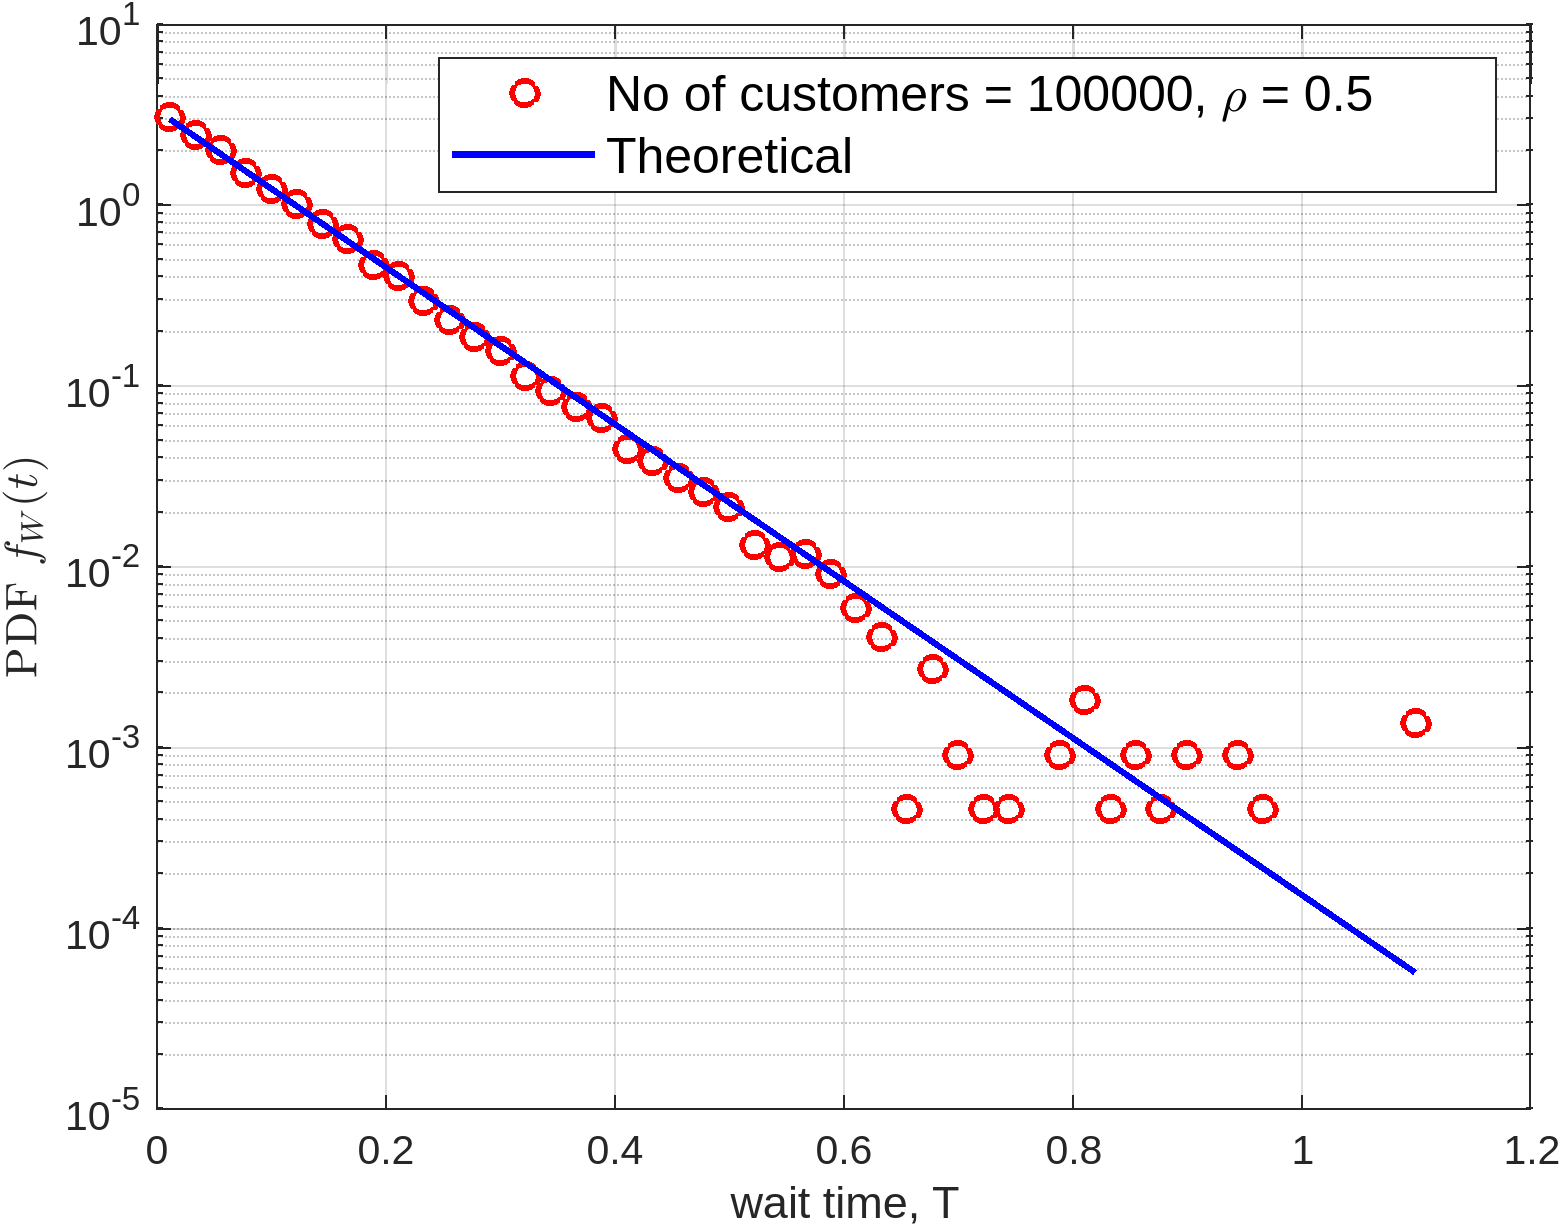
\includegraphics[width=200px]{../code/figures/waiting_time_dist/semilogy_plot_no_customers_100000_rho_0.5.png}
  }
  \caption{PDF of the waiting time in the system for low and medium $\rho$}  
  \label{PDF_W_low_med}
\end{figure}

\begin{figure}[H]
  \centering
  \subfloat[]{
    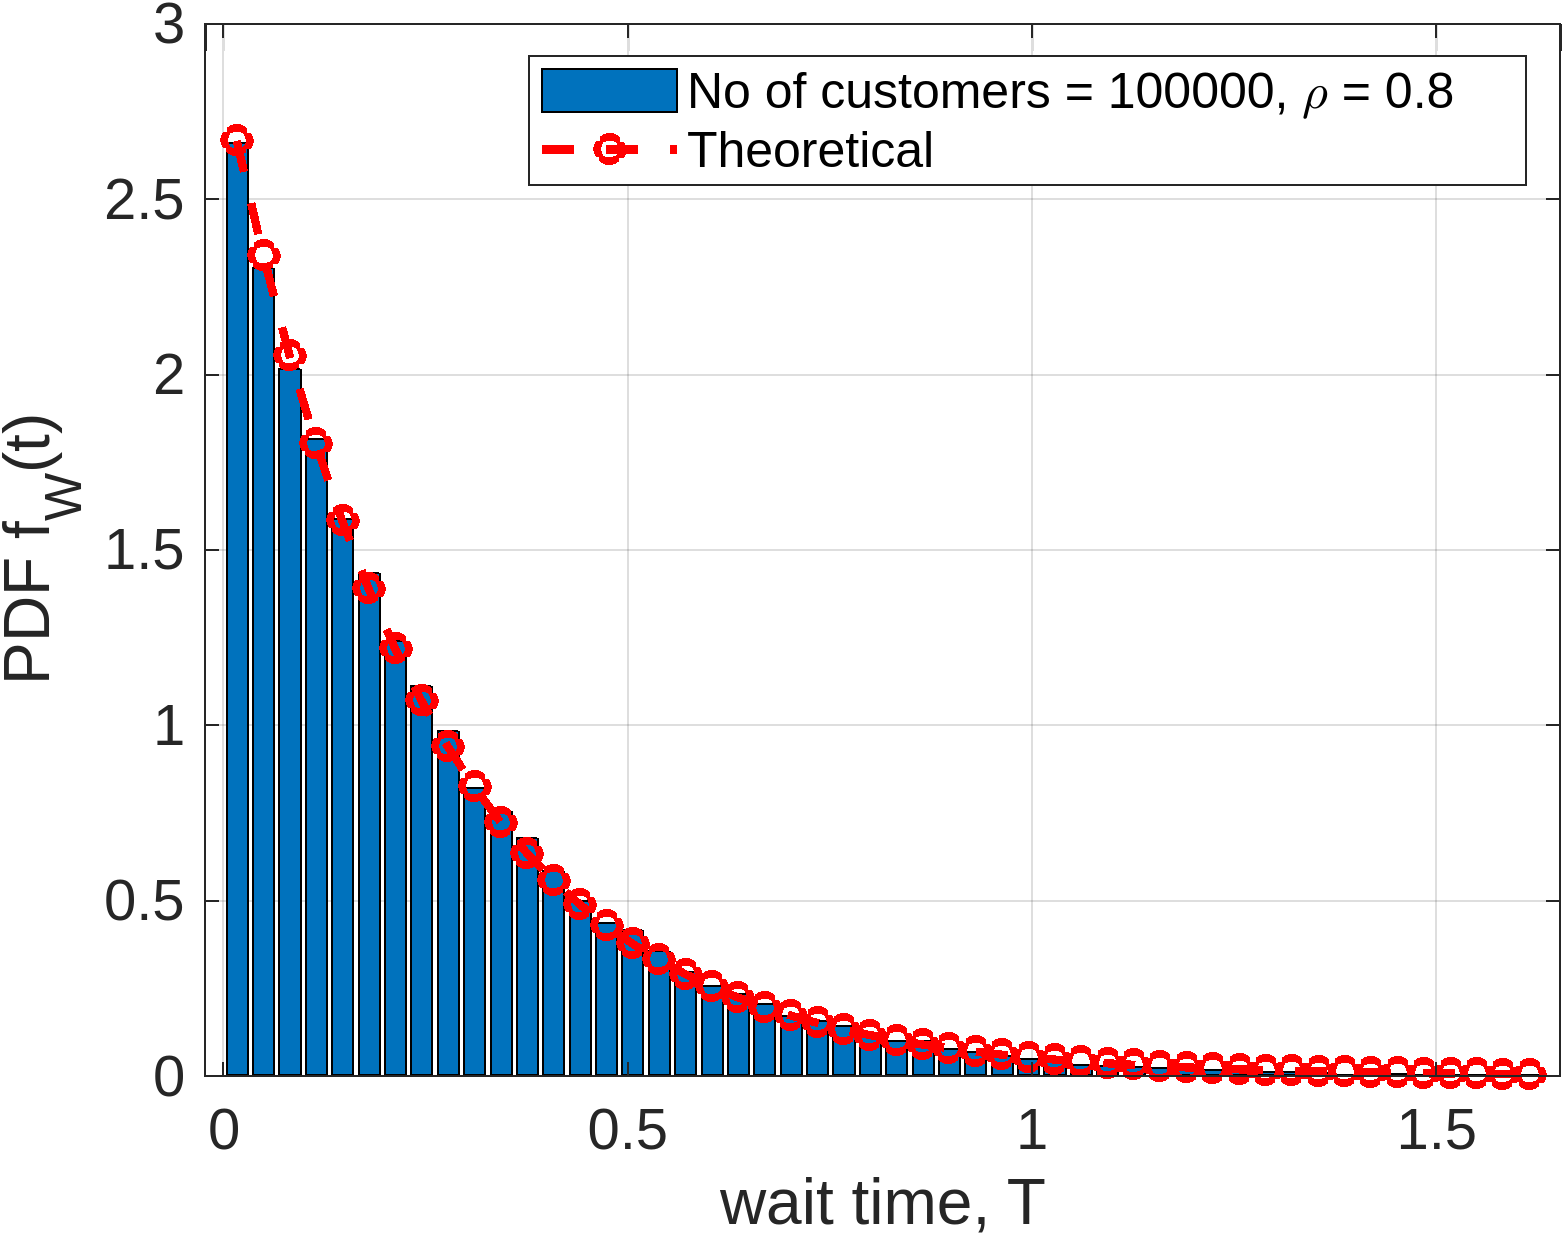
\includegraphics[width=200px]{../code/figures/waiting_time_dist/bar_plot_no_customers_100000_rho_0.8.png}
  }
  \subfloat[]{
    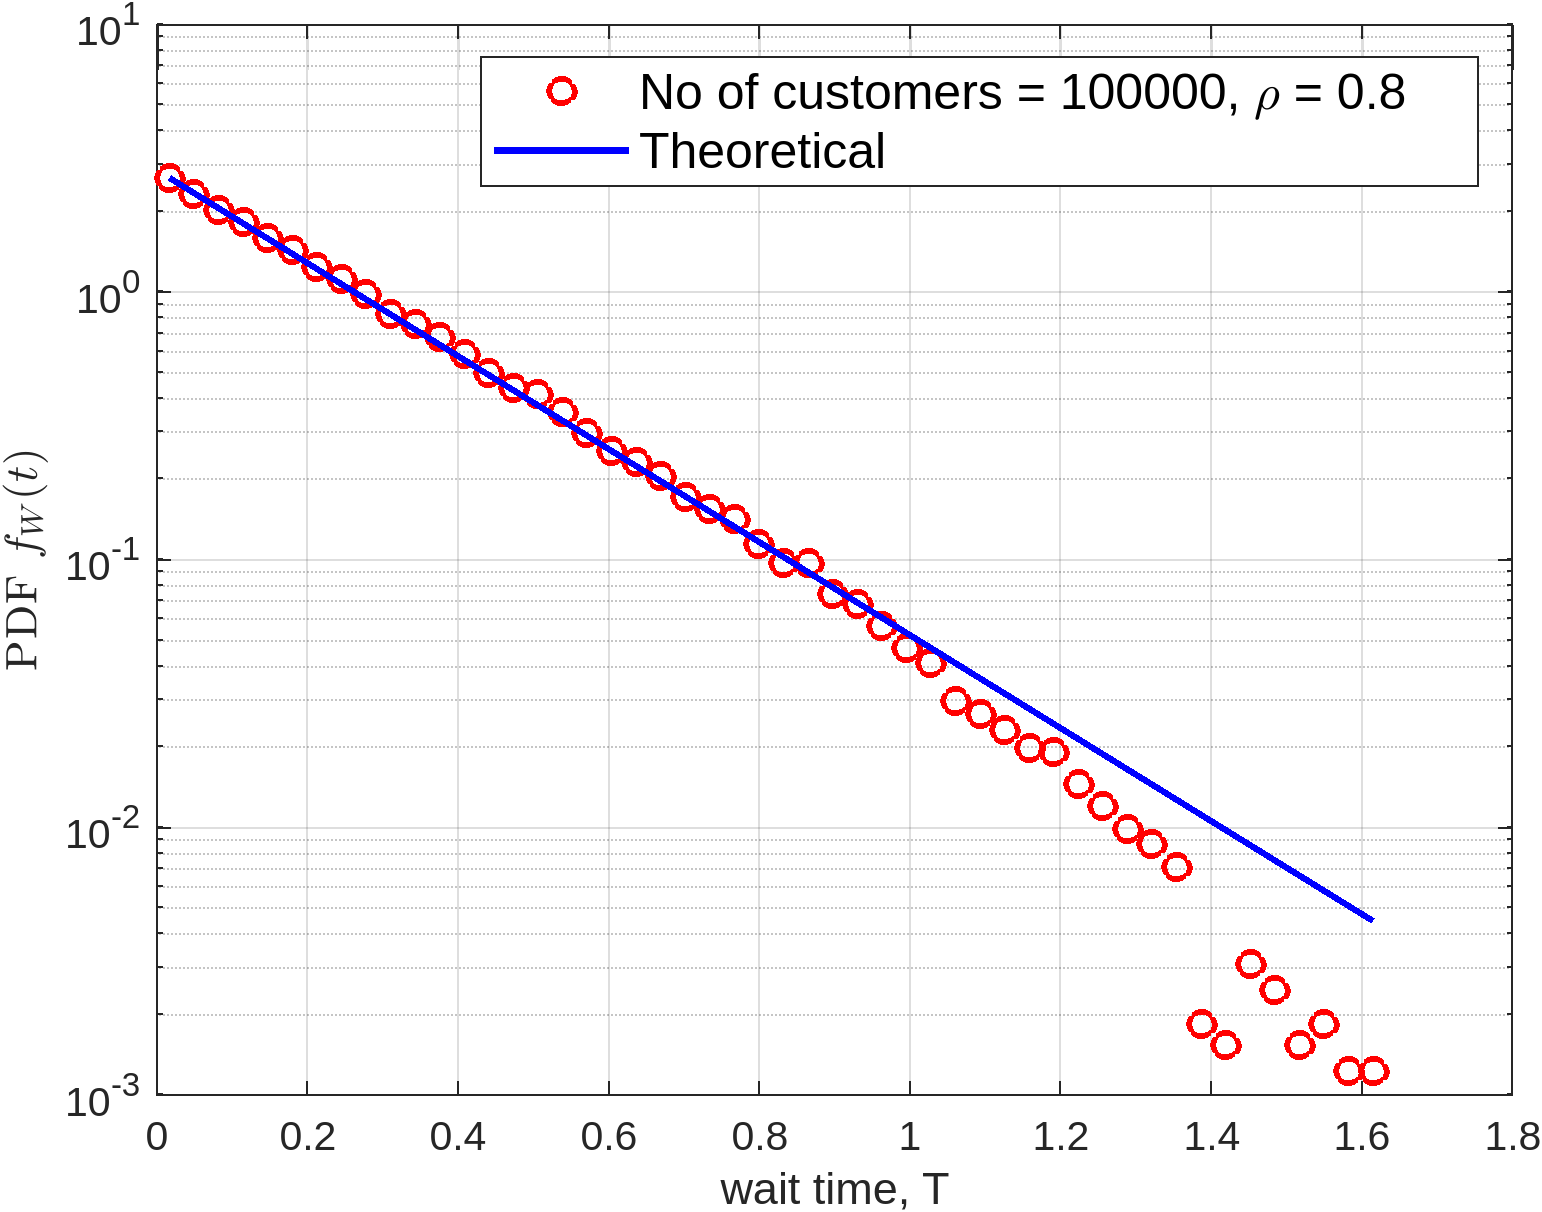
\includegraphics[width=200px]{../code/figures/waiting_time_dist/semilogy_plot_no_customers_100000_rho_0.8.png}
  }
  \hspace{0px}
  \subfloat[]{
    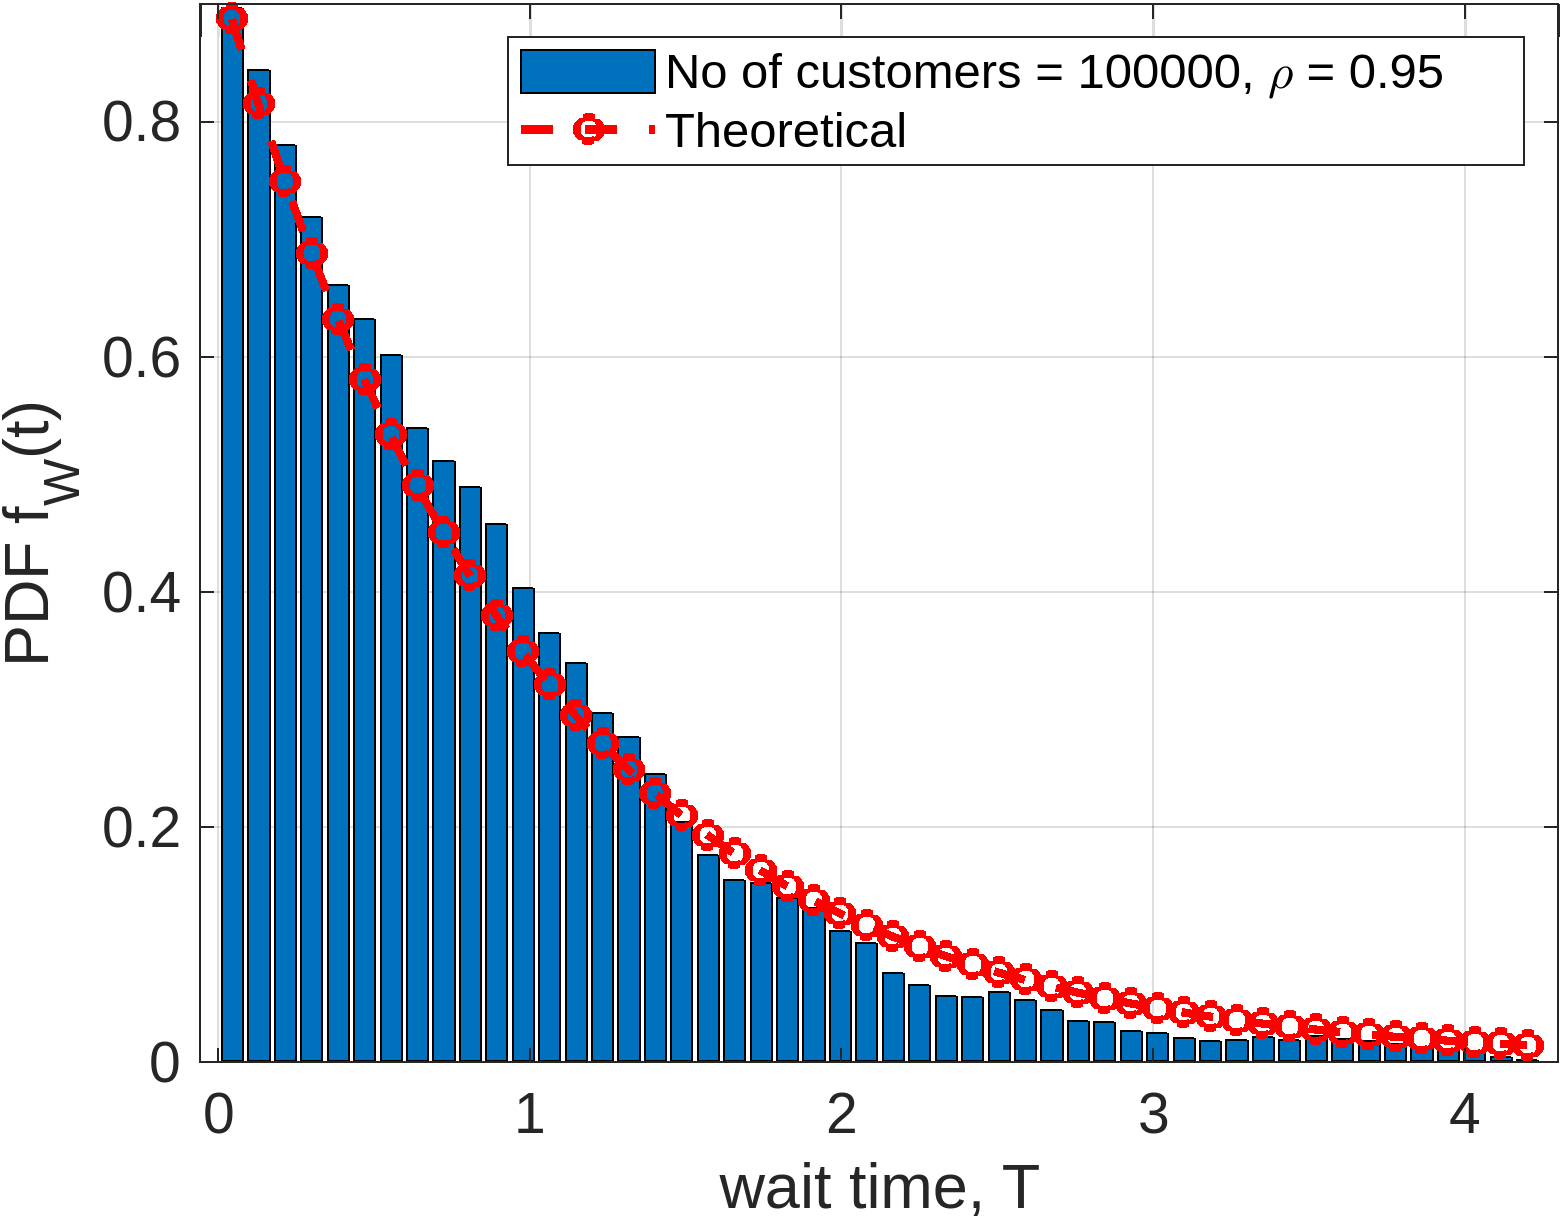
\includegraphics[width=200px]{../code/figures/waiting_time_dist/bar_plot_no_customers_100000_rho_0.95.png}
  }
  \subfloat[]{
    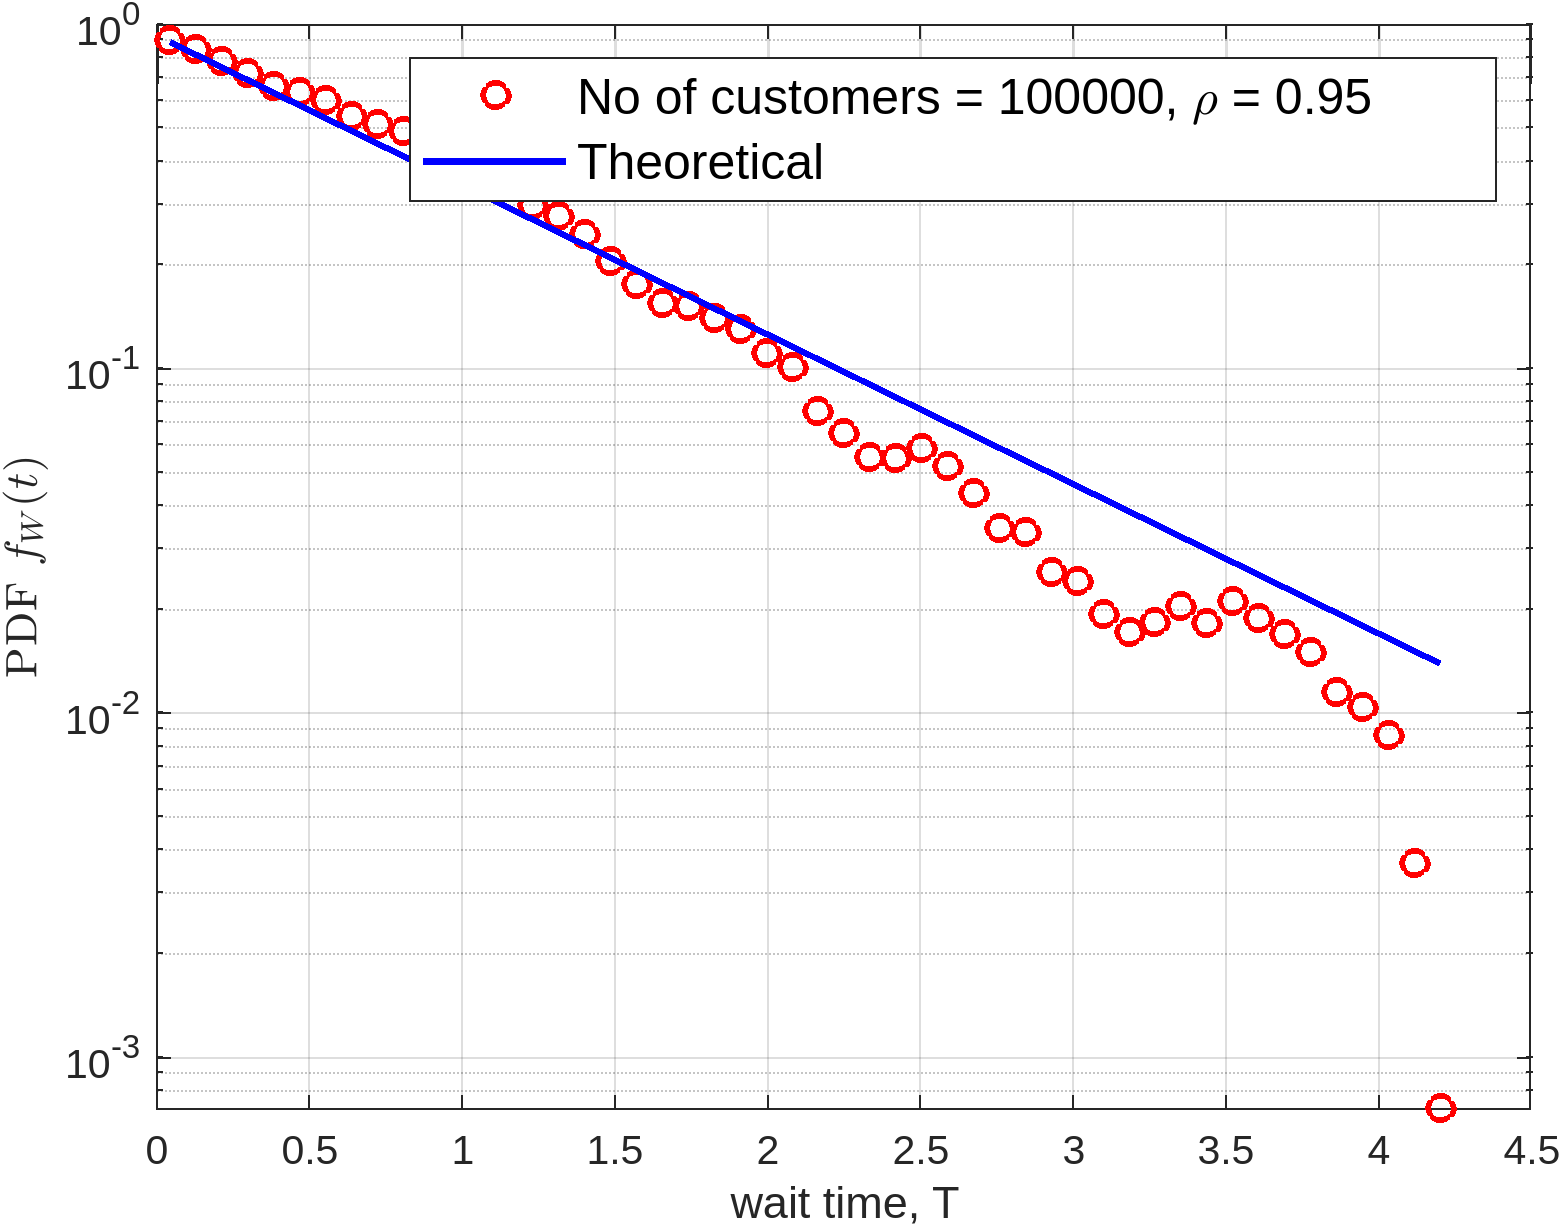
\includegraphics[width=200px]{../code/figures/waiting_time_dist/semilogy_plot_no_customers_100000_rho_0.95.png}
  }
  \caption{PDF of the waiting time in the system for high $\rho$}  
  \label{PDF_W_high}
\end{figure}

Figure \ref{PDF_W_low_med} shows the PDF of the waiting time for low traffic intensity, $\rho=0.25$
and a medium traffic intensity, $\rho=0.5$. They are exponentially distributed, and they match with
theoretical distributions. Figure \ref{PDF_W_high} indicates the distribution of the waiting time
for high intensities $rho =0.8$ and $\rho=0.95$. The plot for $\rho=0.8$ is in relatively excellent 
agreement with the theoretical one, but the plot $\rho =0.95$ is slightly far from the theoretical 
PDF. We have increased the number of customers for the high intensity case to $1000000$ customers
and the results have improved as shown in Figure \ref{PDF_W_high_more_cust}.

\begin{figure}[H]
  \centering
  \subfloat[]{
    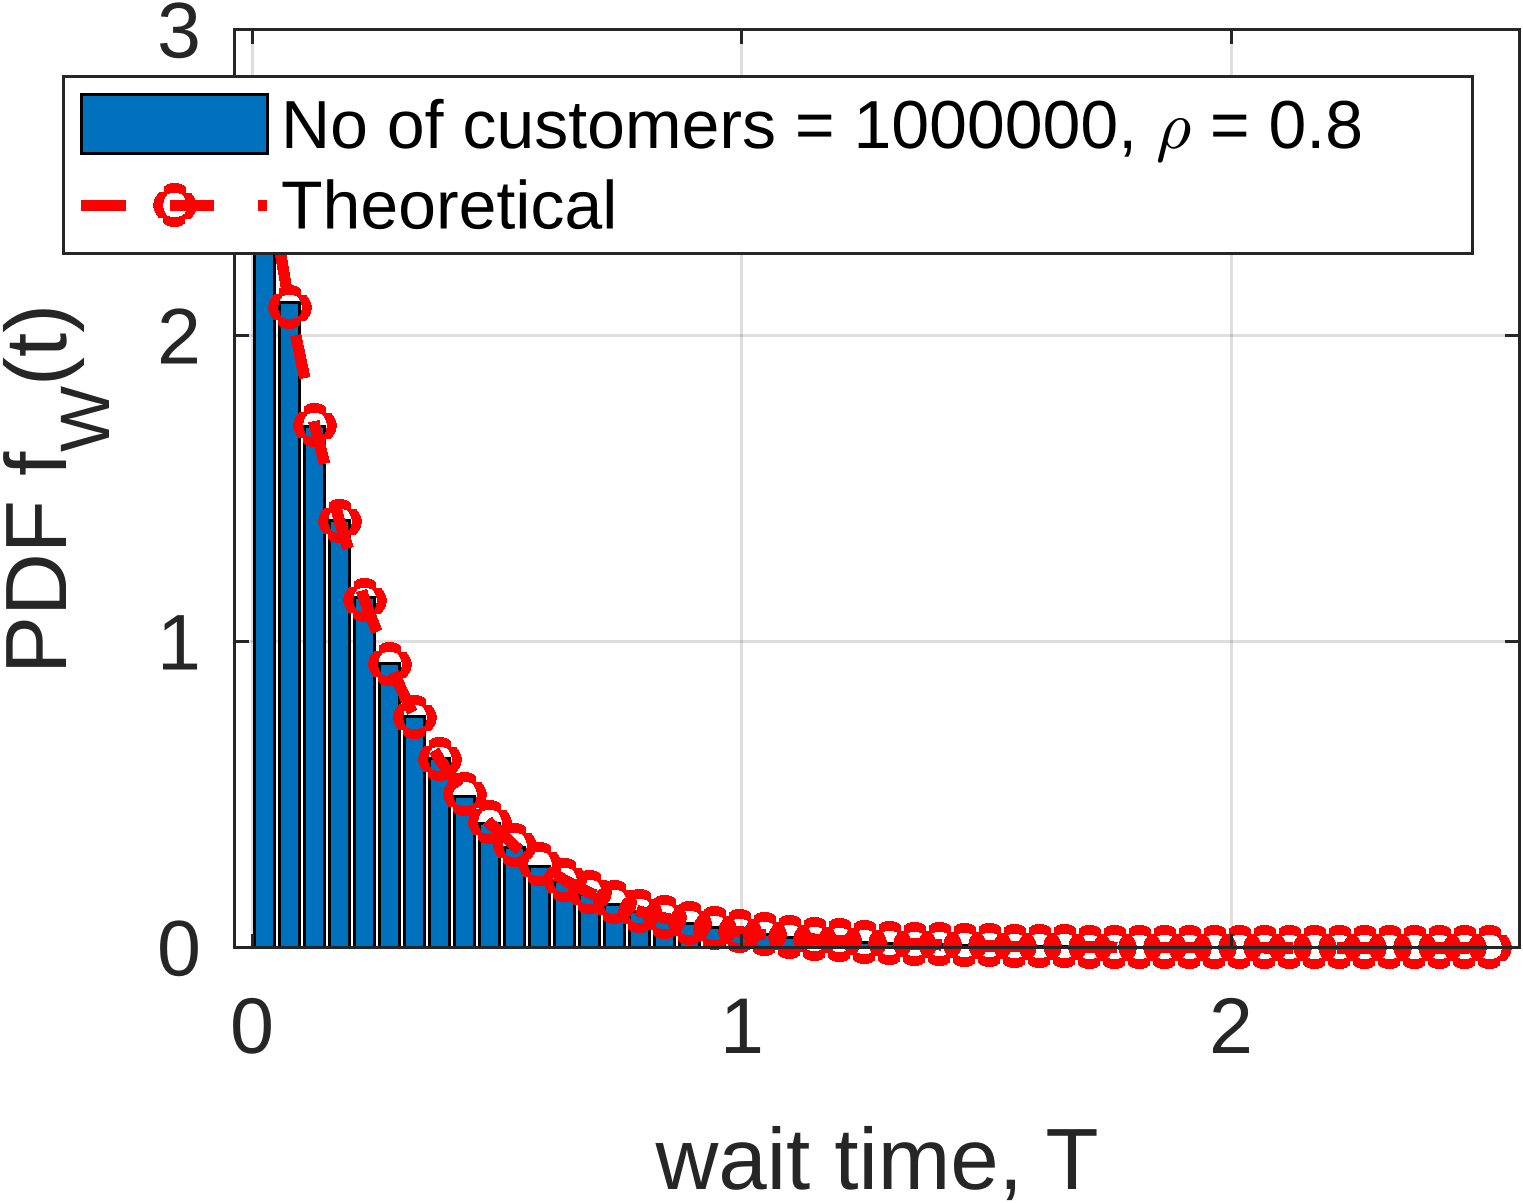
\includegraphics[width=200px]{../code/figures/waiting_time_dist/bar_plot_no_customers_1000000_rho_0.8.png}
  }
  \subfloat[]{
    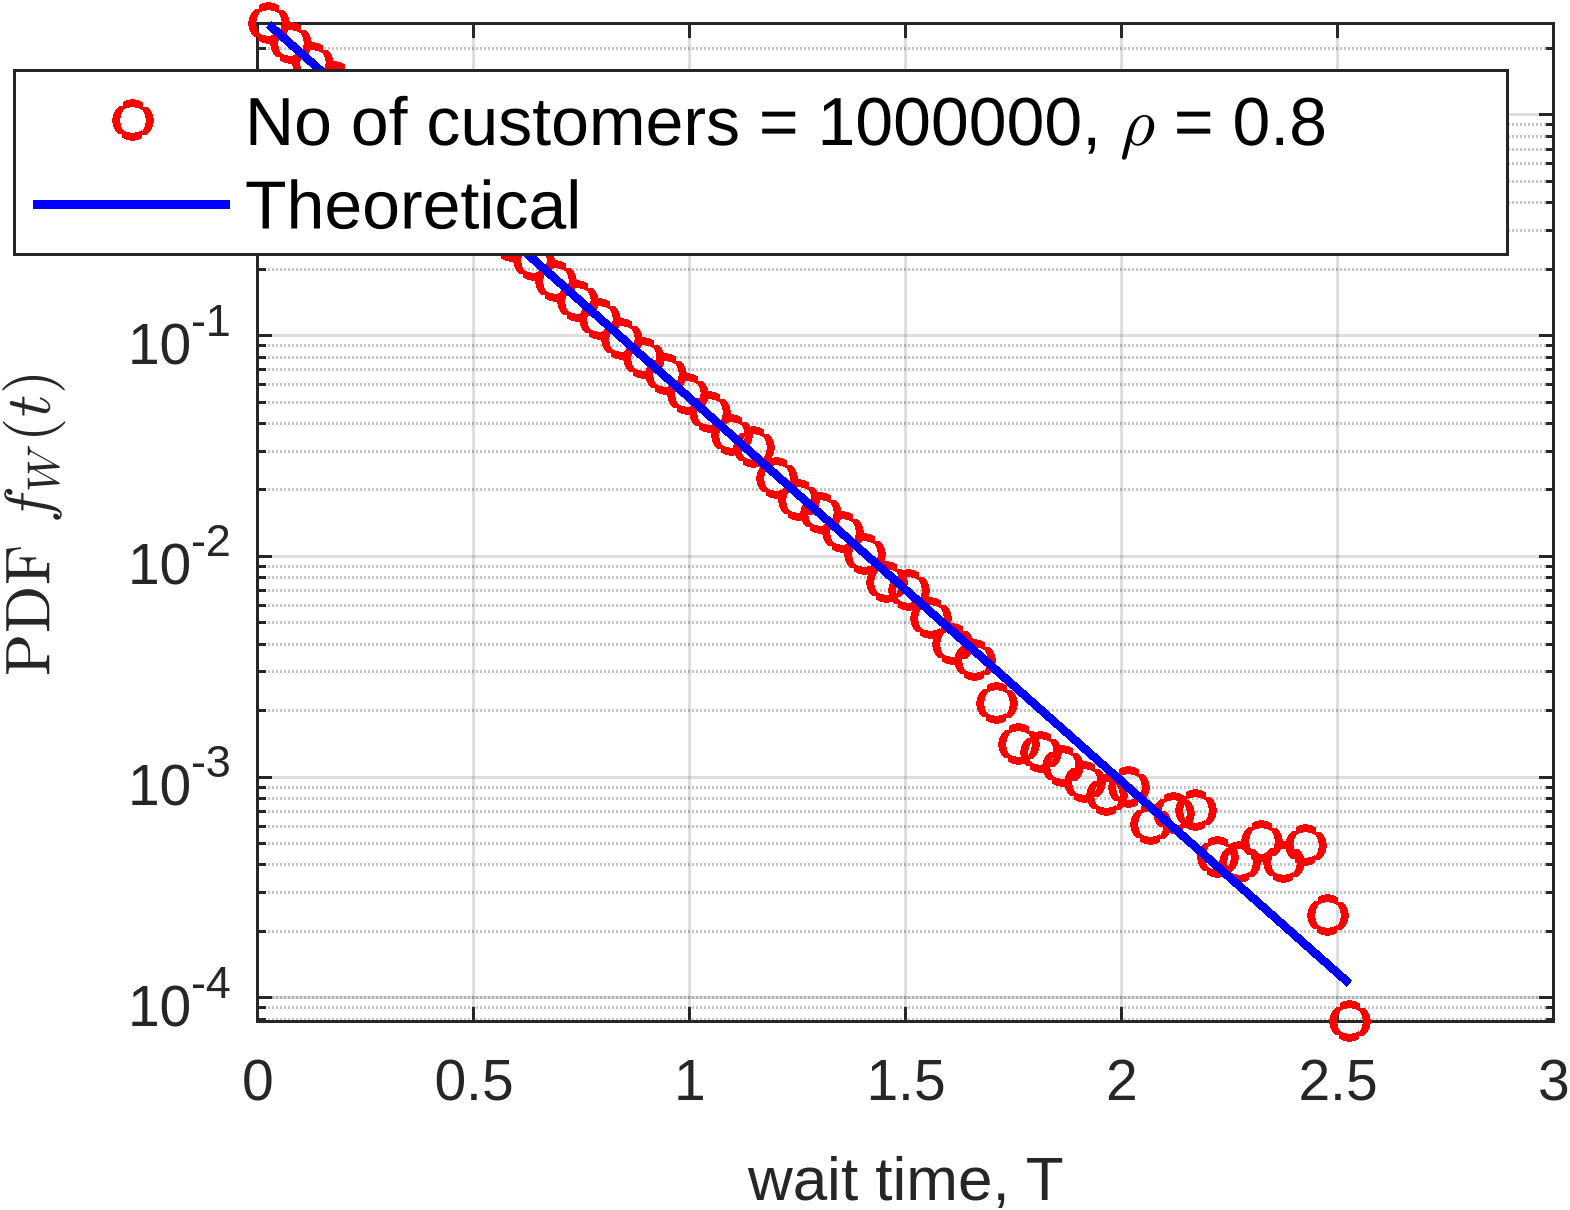
\includegraphics[width=200px]{../code/figures/waiting_time_dist/semilogy_plot_no_customers_1000000_rho_0.8.png}
  }
  \hspace{0px}
  \subfloat[]{
    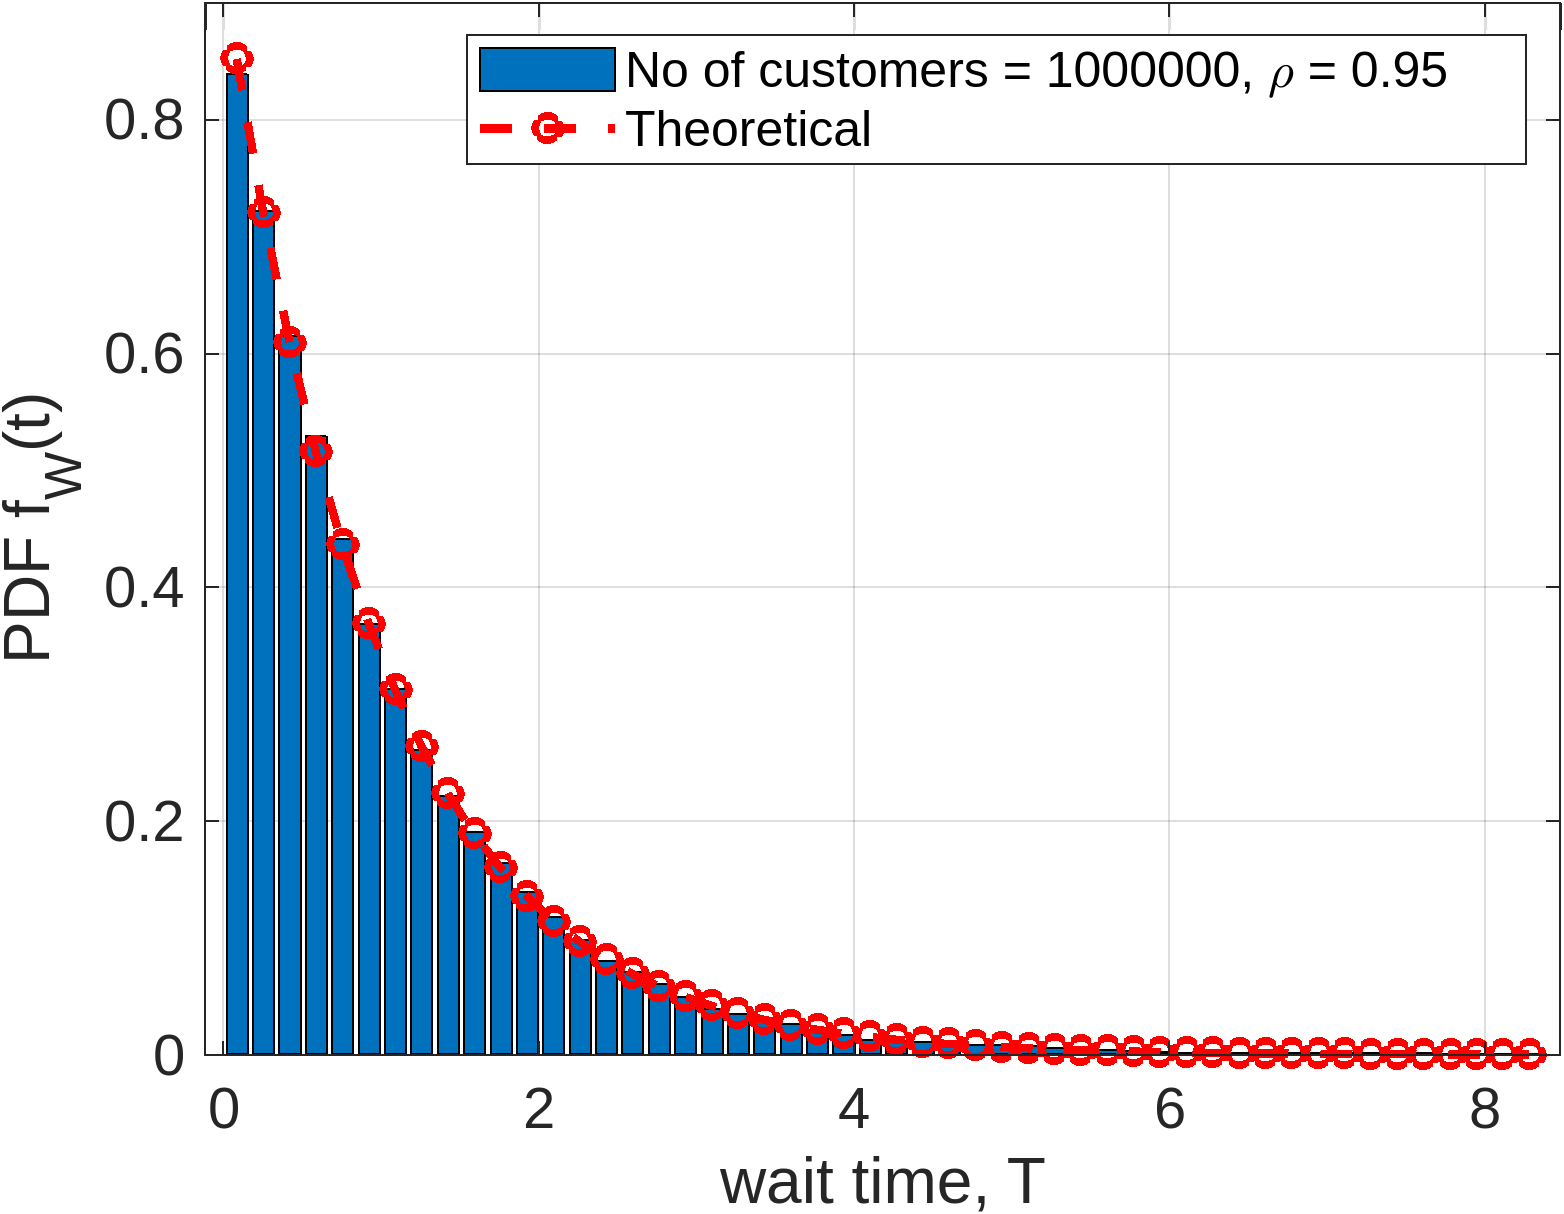
\includegraphics[width=200px]{../code/figures/waiting_time_dist/bar_plot_no_customers_1000000_rho_0.95.png}
  }
  \subfloat[]{
    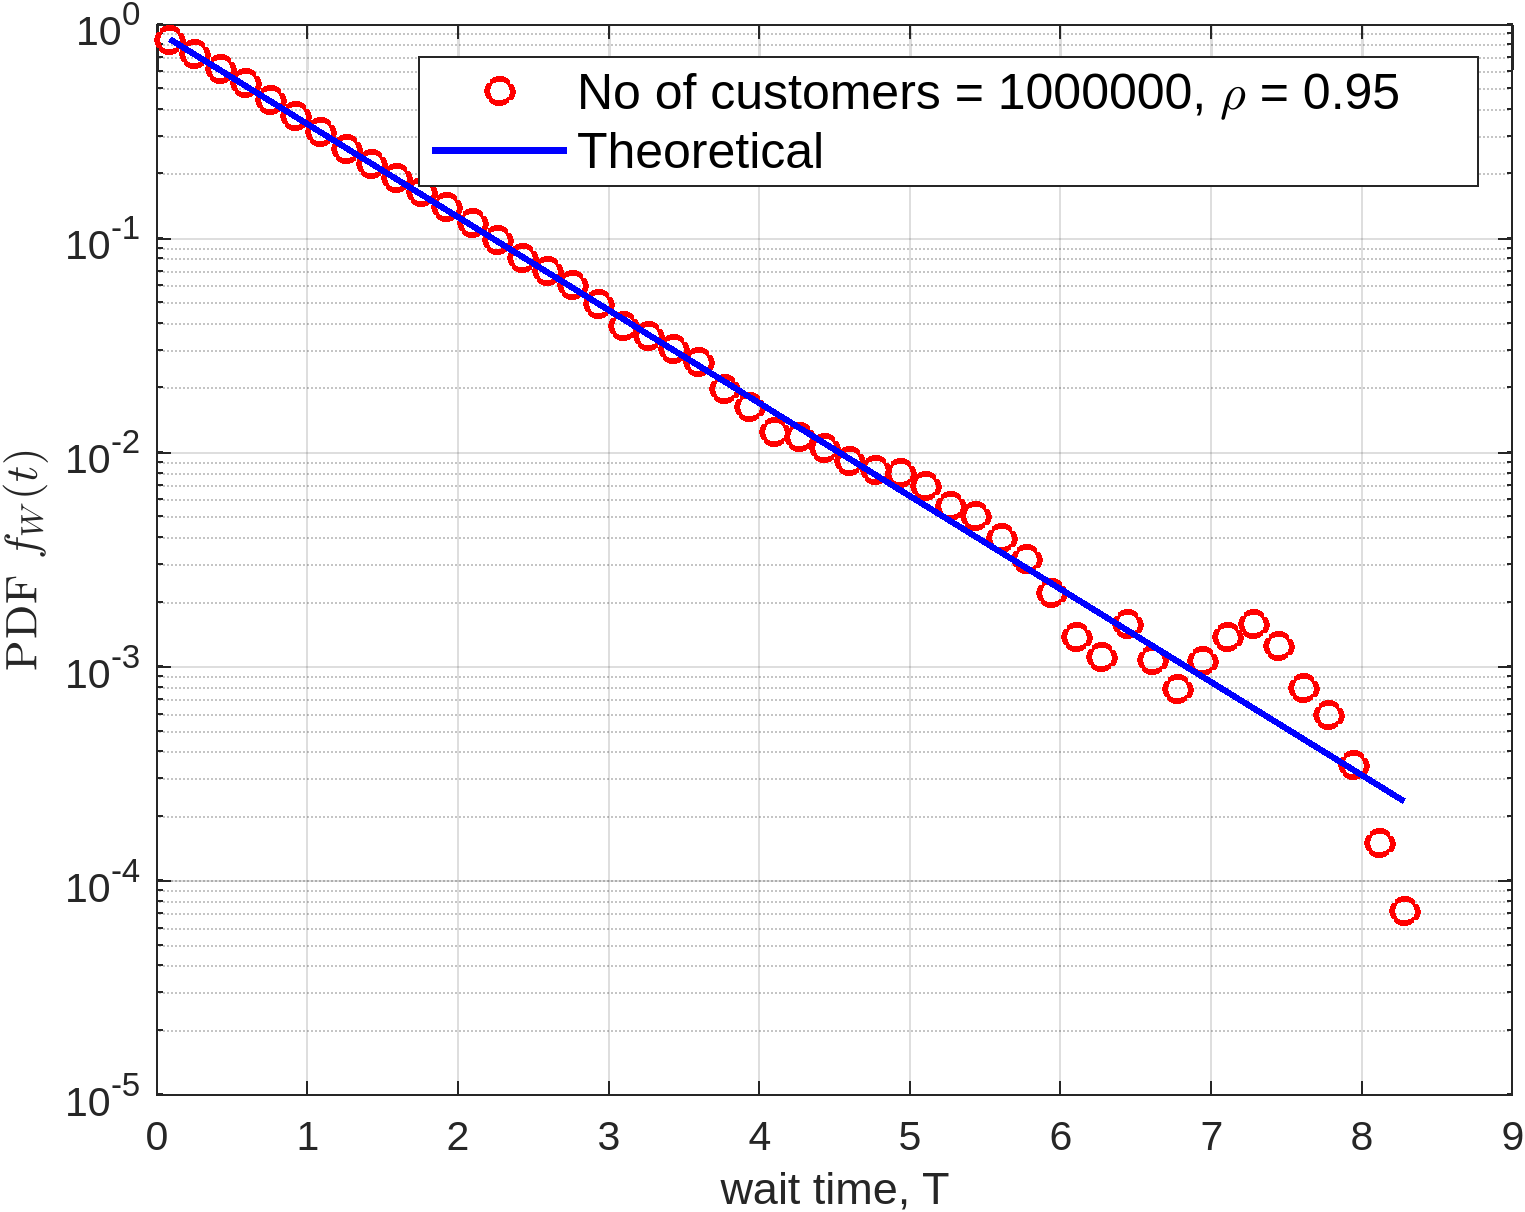
\includegraphics[width=200px]{../code/figures/waiting_time_dist/semilogy_plot_no_customers_1000000_rho_0.95.png}
  }
  \caption{PDF of the waiting time in the system for high $\rho$}  
  \label{PDF_W_high_more_cust}
\end{figure}

\subsection{PMF of $N(t)$}
\begin{figure}[H]
  \centering
  \subfloat[]{
    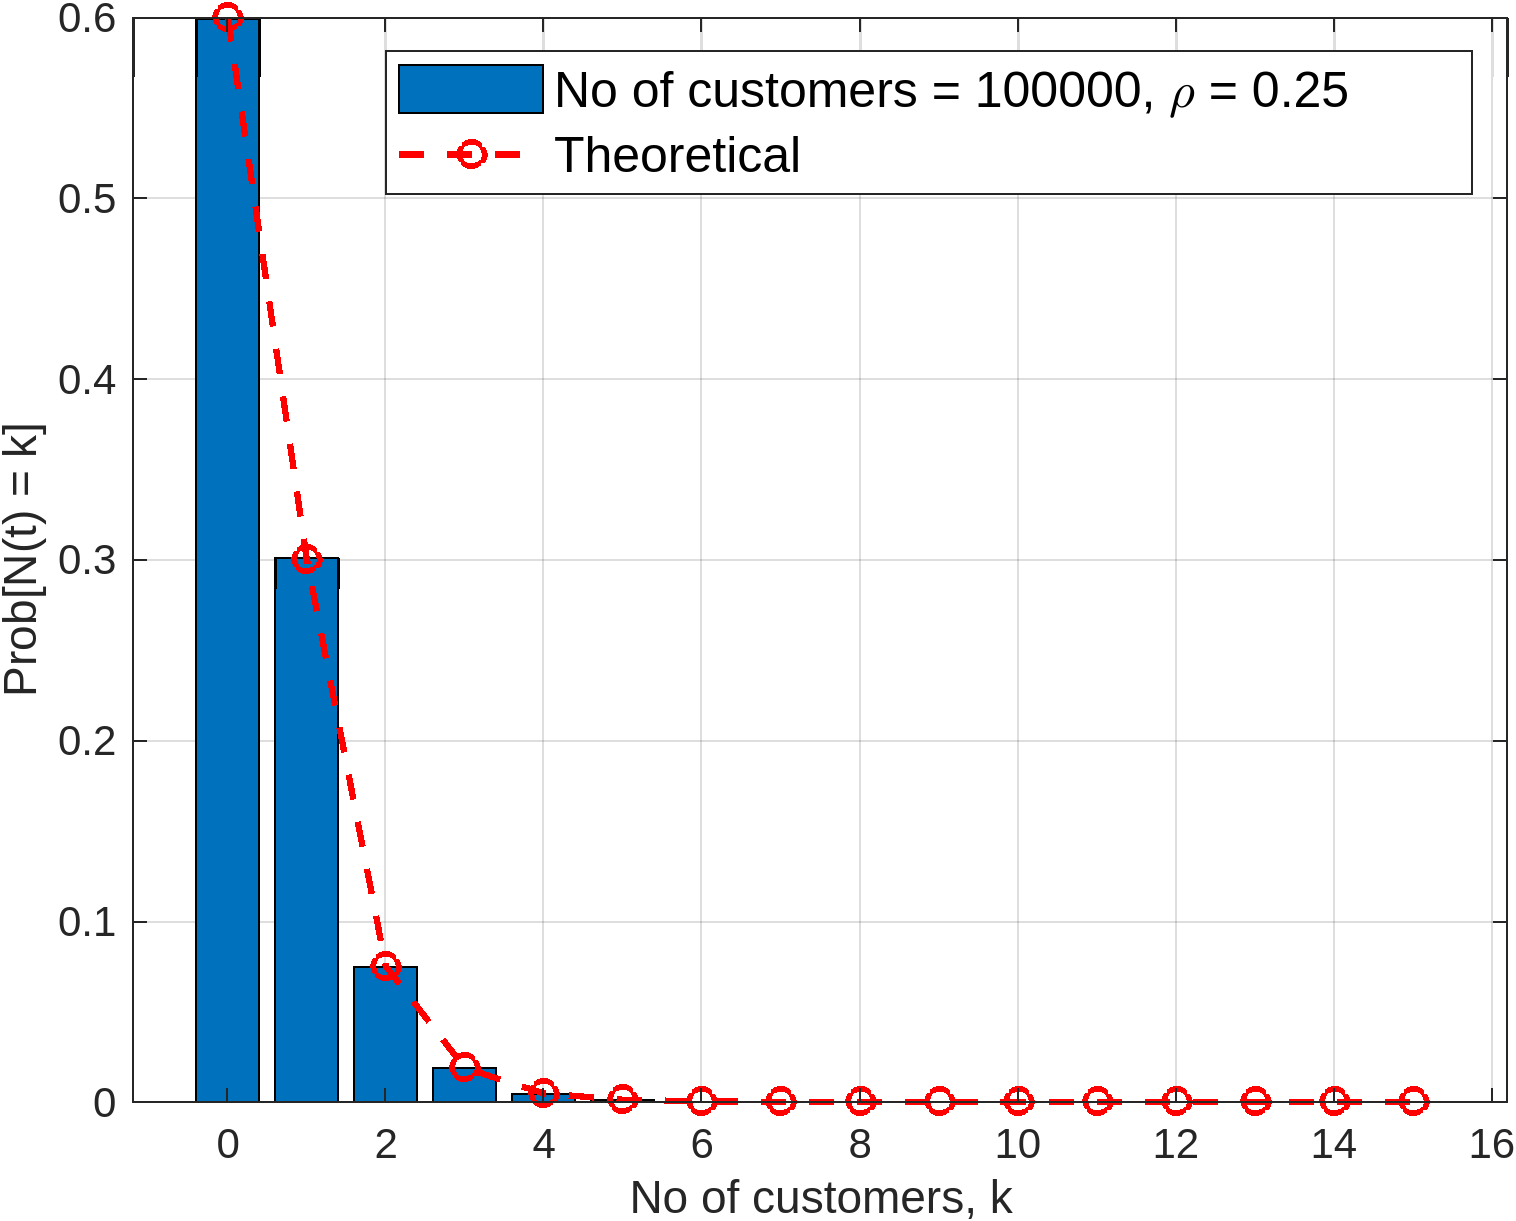
\includegraphics[width=200px]{../code/figures/N_PMF/semilogy_plot_no_customers_100000_rho_0.25.png}
  }
  \subfloat[]{
    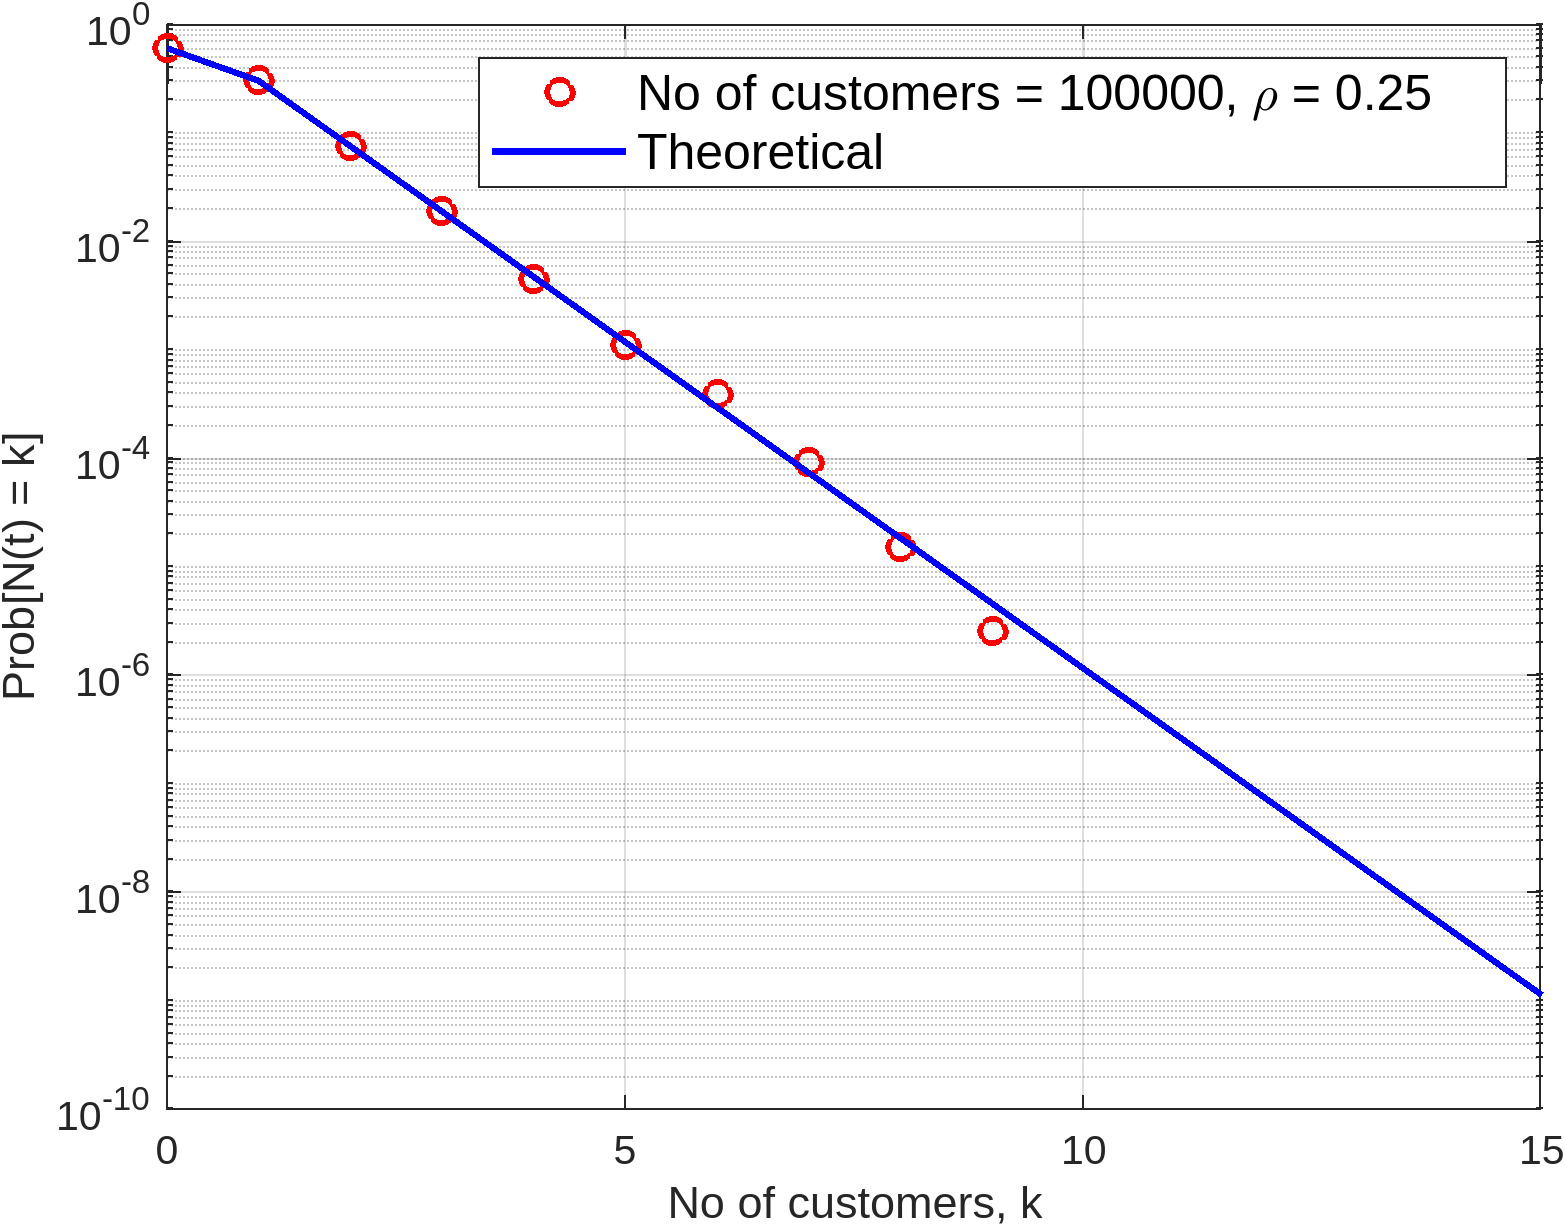
\includegraphics[width=200px]{../code/figures/N_PMF/bar_plot_no_customers_100000_rho_0.25.png}
  }
  \hspace{0px}
  \subfloat[]{
    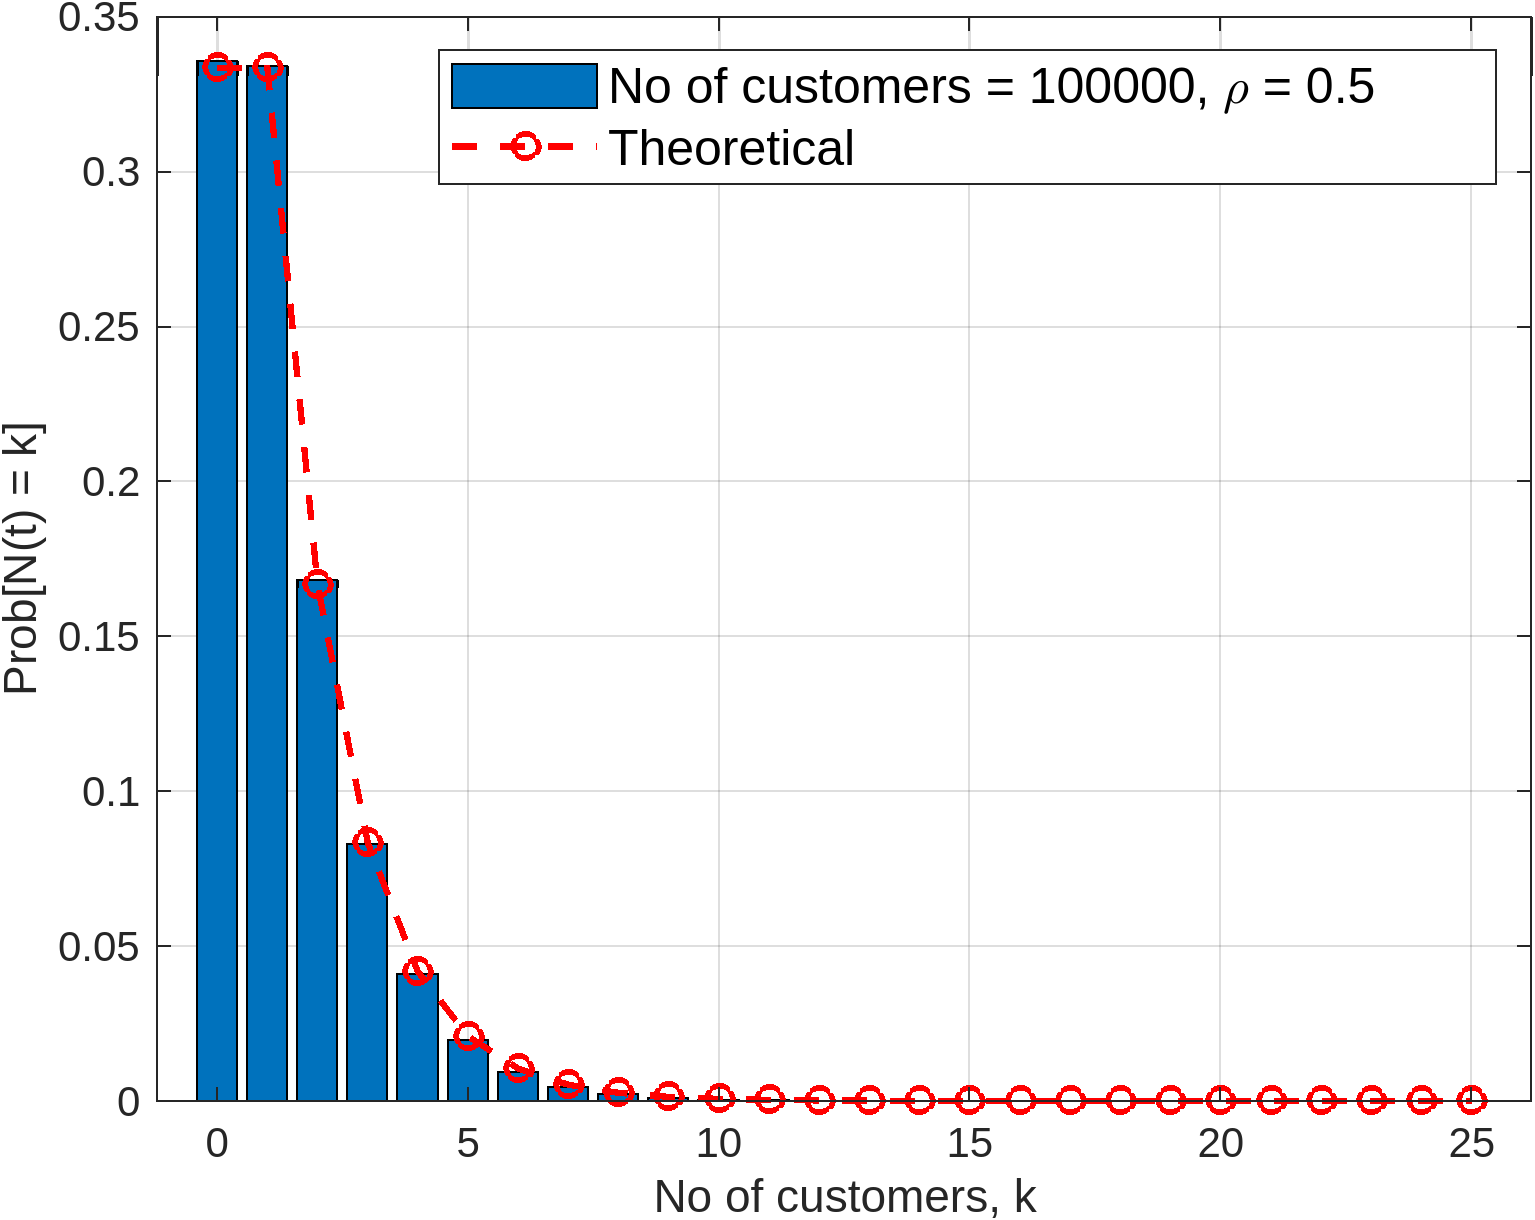
\includegraphics[width=200px]{../code/figures/N_PMF/semilogy_plot_no_customers_100000_rho_0.5.png}
  }
  \subfloat[]{
    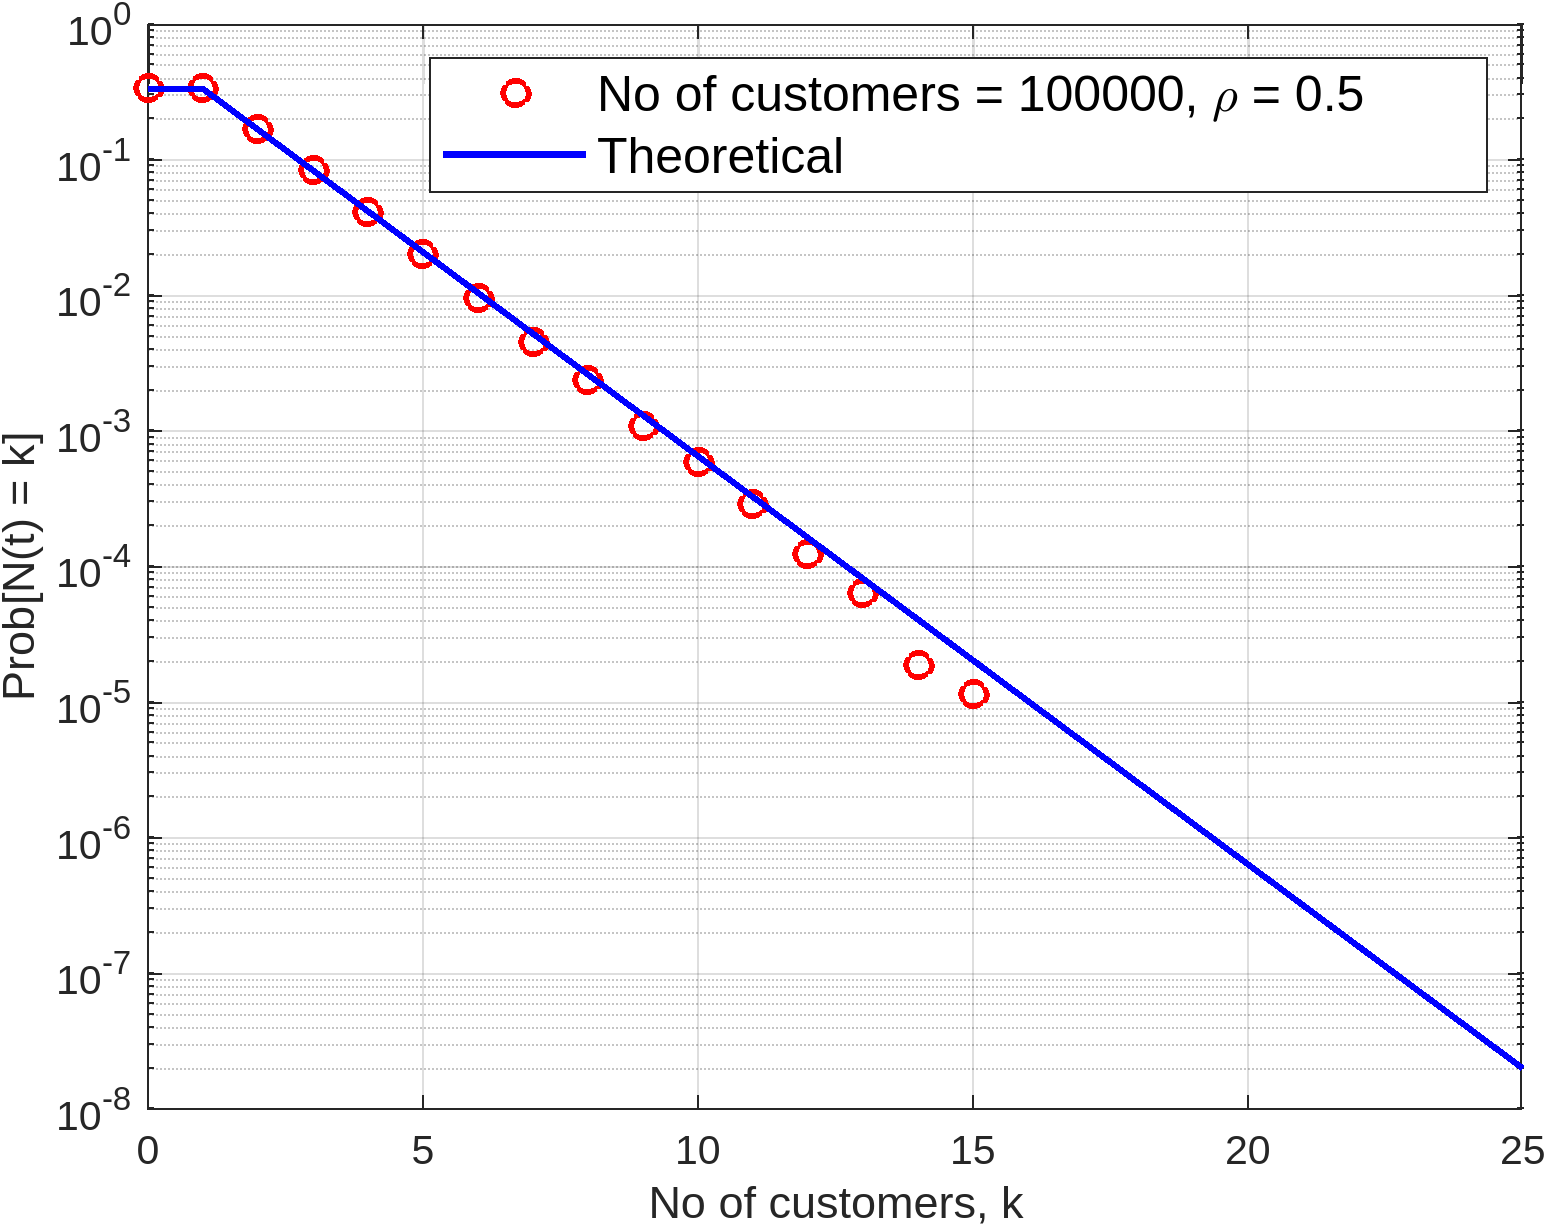
\includegraphics[width=200px]{../code/figures/N_PMF/bar_plot_no_customers_100000_rho_0.5.png}
  }
  \caption{PMF of $N(t)$  for low and medium traffic intensities}  
  \label{PMF_N_low_med}
\end{figure}

\begin{figure}[H]
  \centering
  \subfloat[]{
    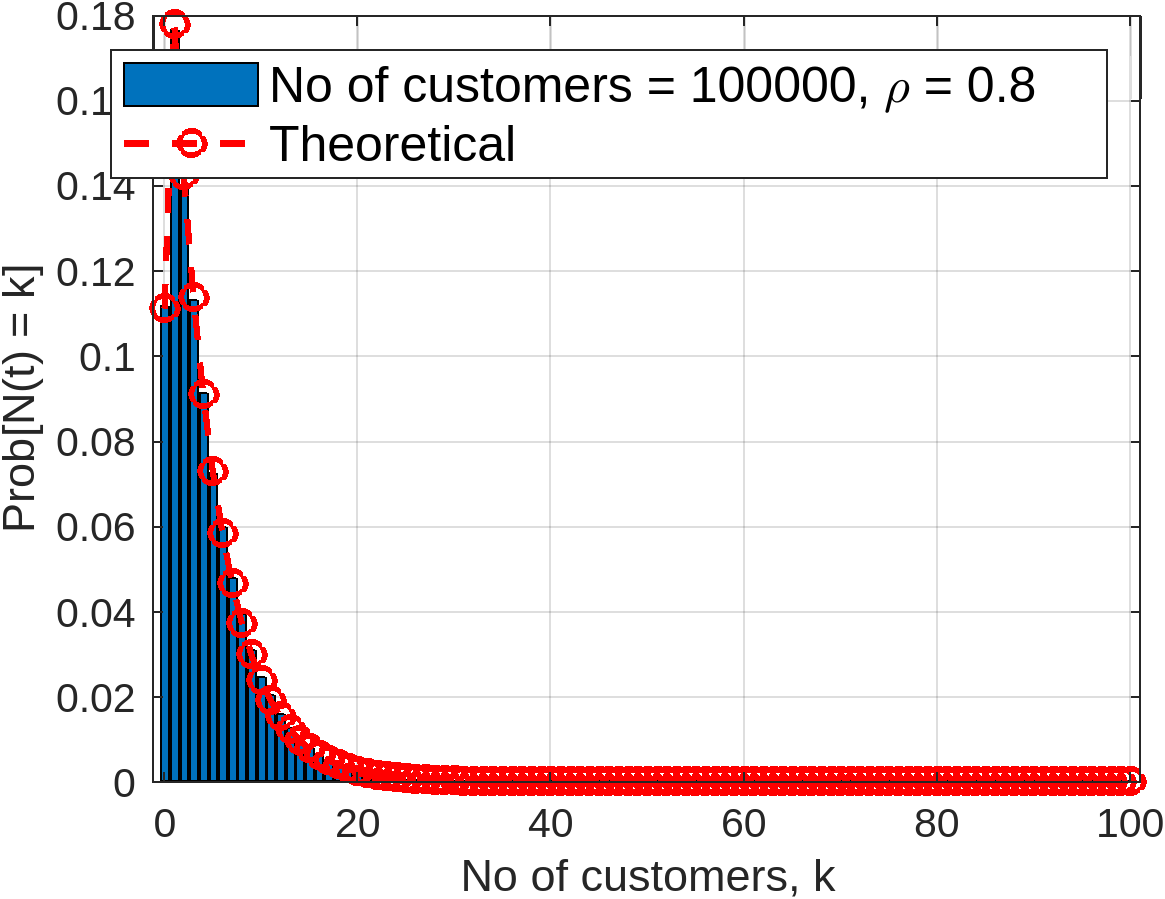
\includegraphics[width=200px]{../code/figures/N_PMF/semilogy_plot_no_customers_100000_rho_0.8.png}
  }
  \subfloat[]{
    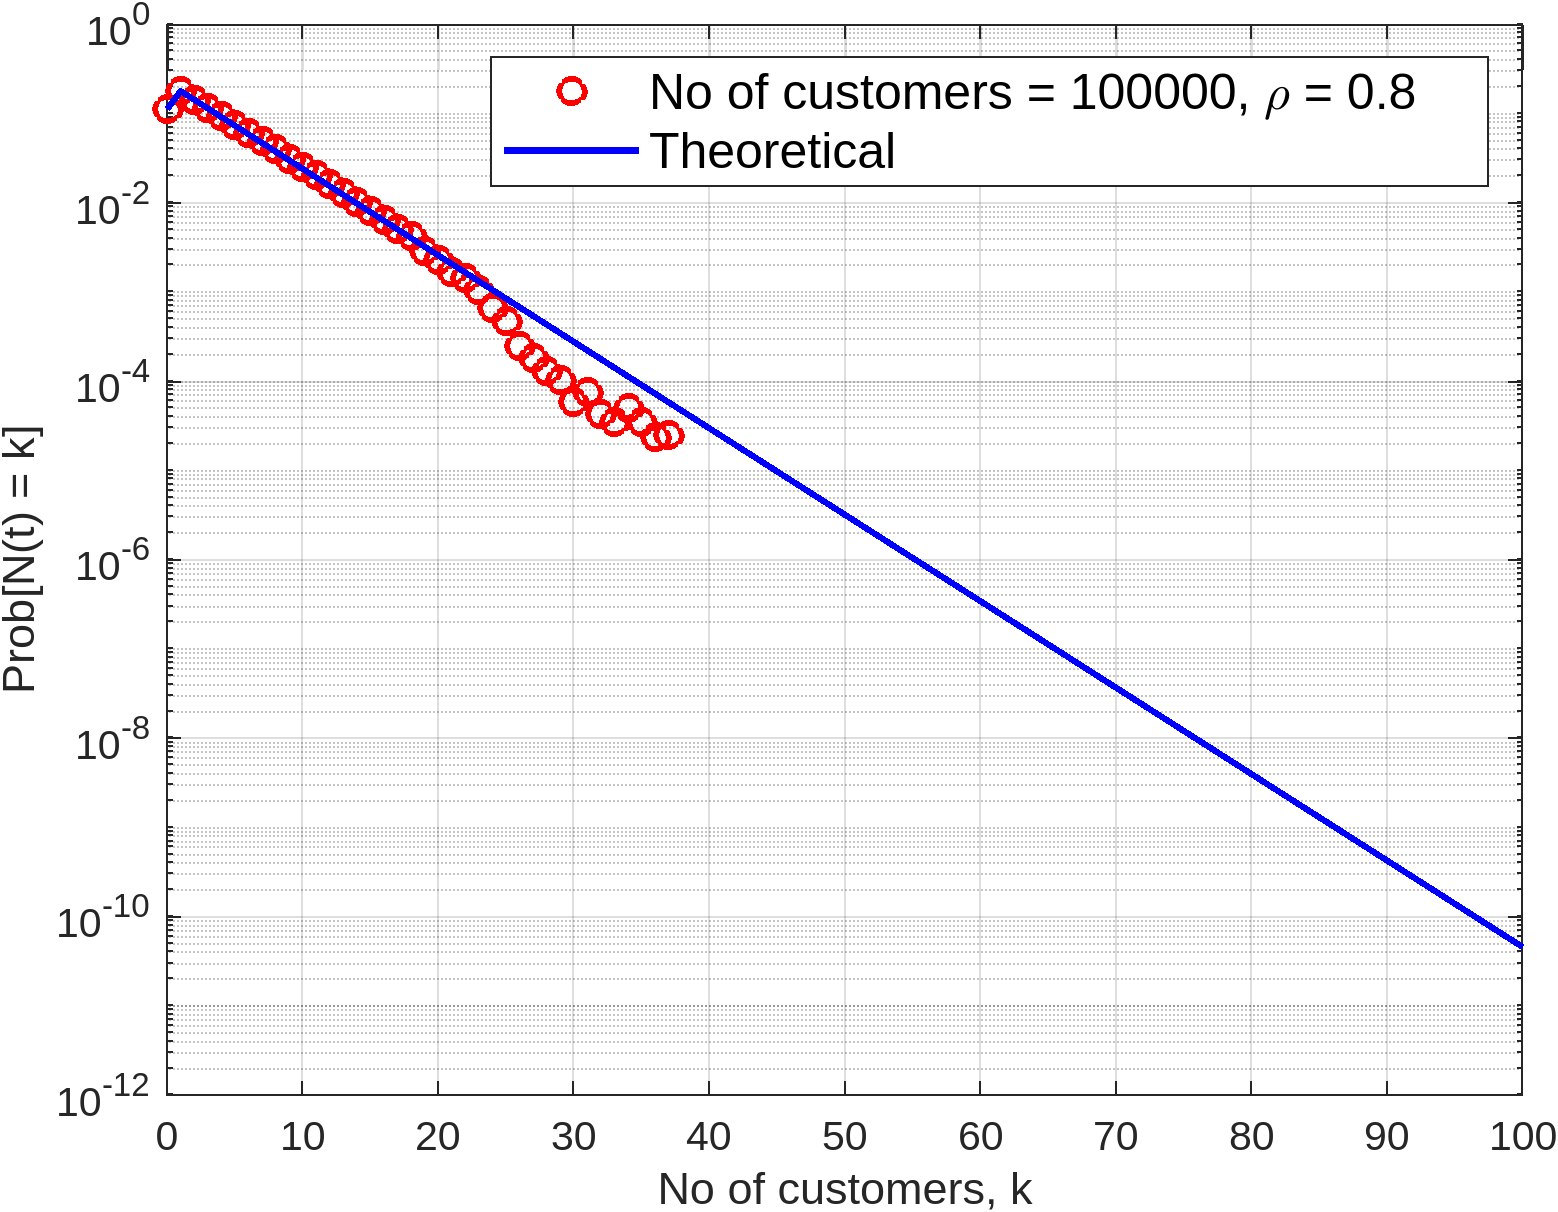
\includegraphics[width=200px]{../code/figures/N_PMF/bar_plot_no_customers_100000_rho_0.8.png}
  }
  \hspace{0px}
  \subfloat[]{
    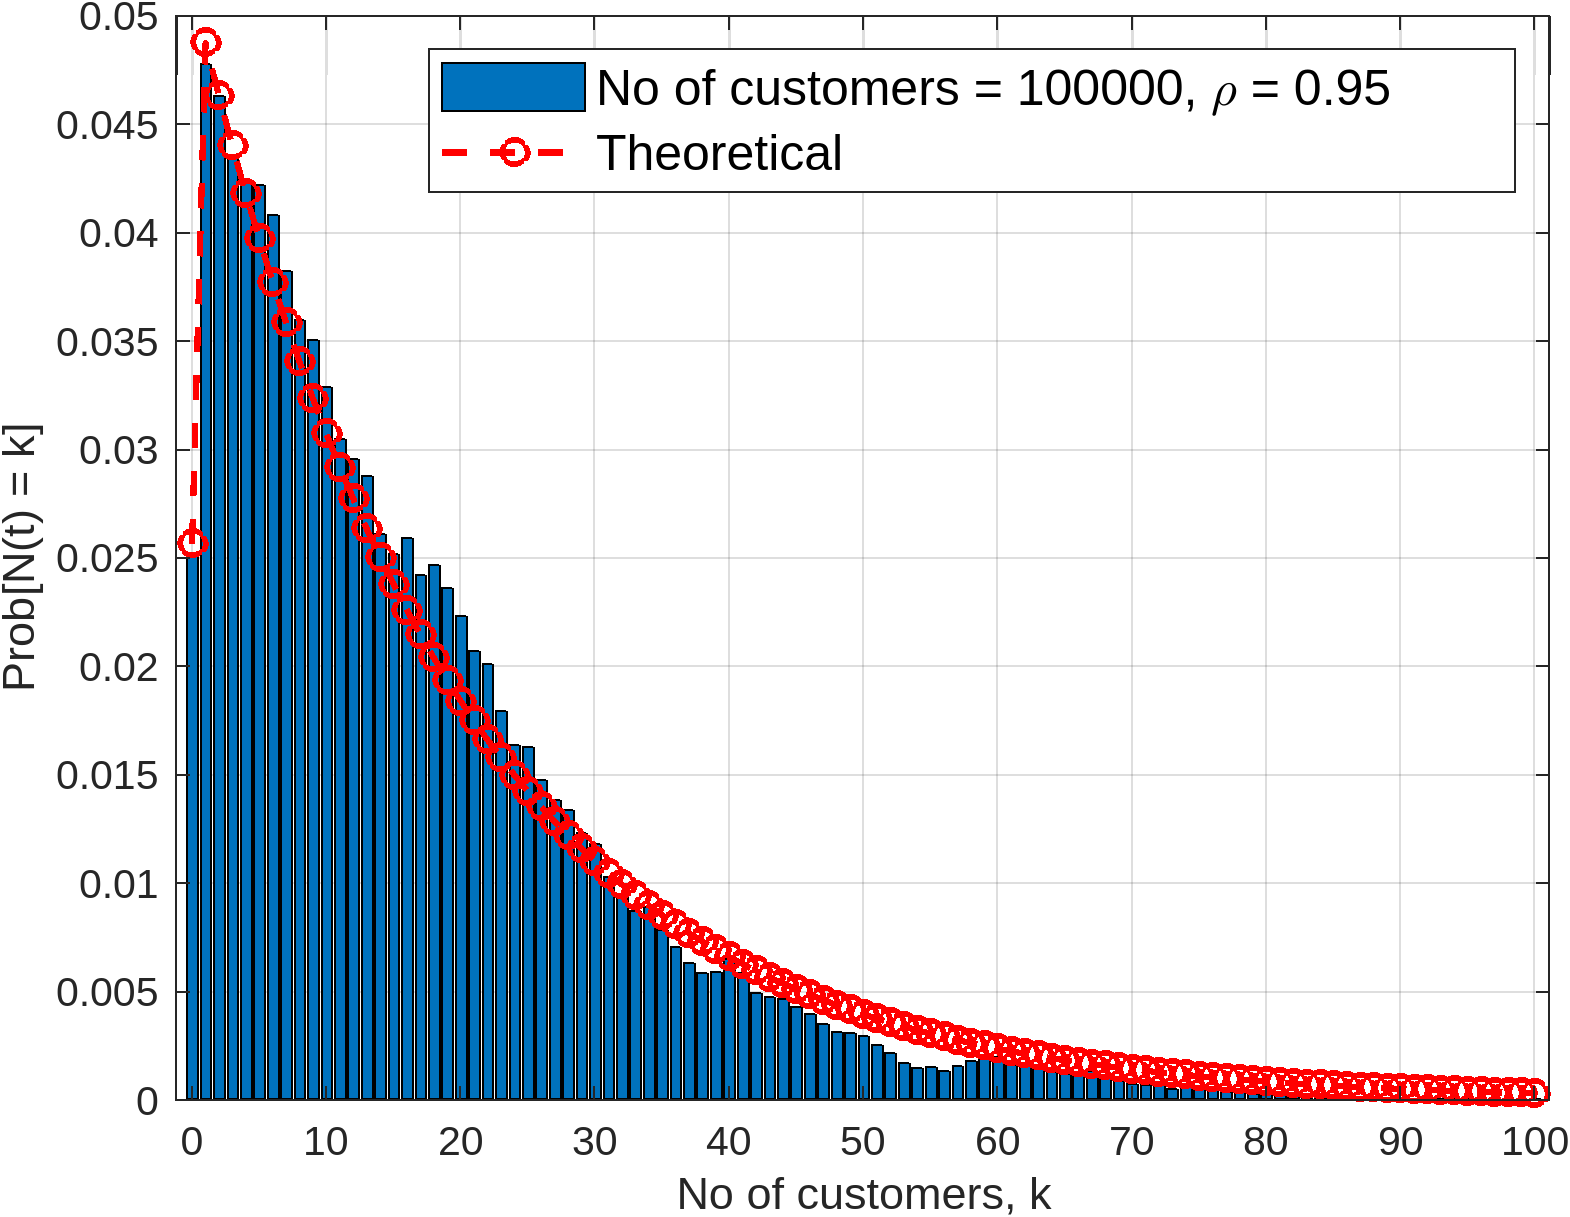
\includegraphics[width=200px]{../code/figures/N_PMF/semilogy_plot_no_customers_100000_rho_0.95.png}
  }
  \subfloat[]{
    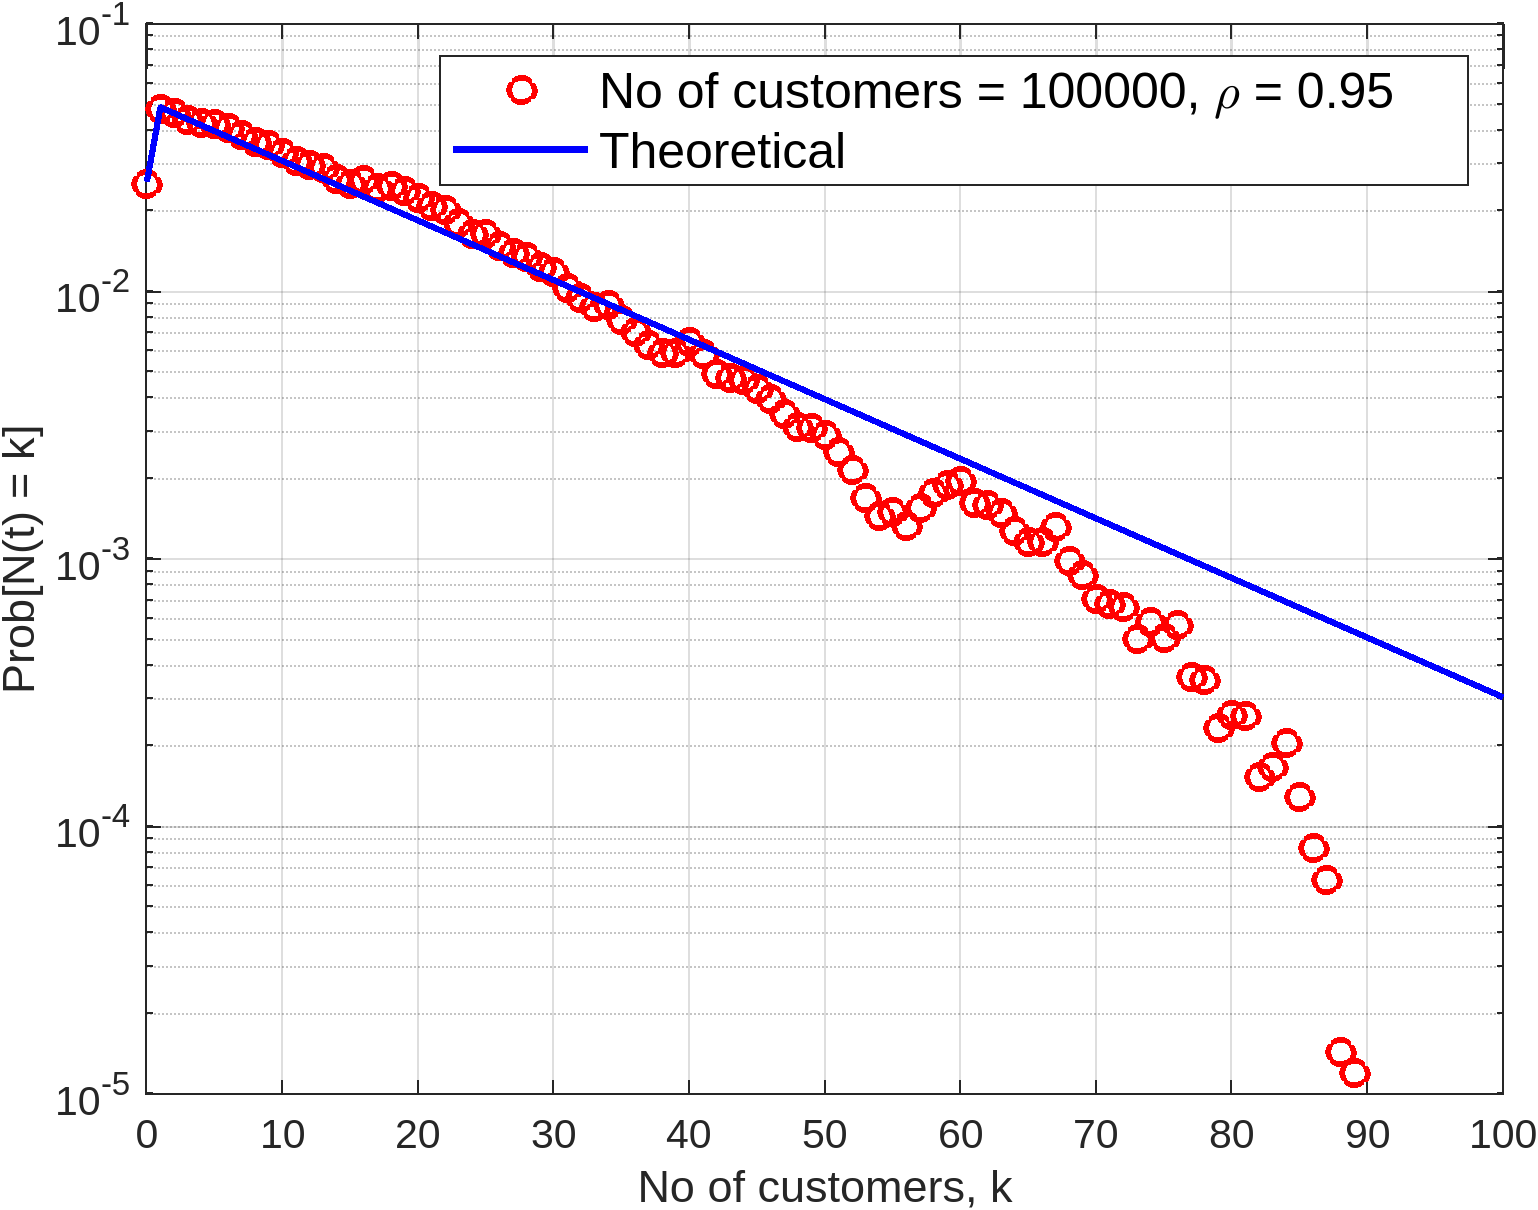
\includegraphics[width=200px]{../code/figures/N_PMF/bar_plot_no_customers_100000_rho_0.95.png}
  }
  \caption{PMF of $N(t)$  for high traffic intensity}  
  \label{PMF_N_high}
\end{figure}

Figure \ref{PMF_N_low_med} shows the probability mass function of the number of
customers in the system for low traffic intensity, $\rho = 0.25$ and medium traffic
intensity, $\rho=0.5$. We noticed that the probability of having 10 customers and more in the 
system for $\rho=0.25$ and the probability of having 15 customers or more in the system is 
almost zero (negligible). The theoretical and the empirical PMF are in an excellent agreement 
with one another. 

Figure \ref{PMF_N_high} show the PMF of $N(t)$ for high intensities, and we notice that the 
probability of having more customers in the system has increased larger from the case of low 
and medium intensities. For $\rho=0.8$, the empirical distributed agrees well with the theoretical
one, but the one for $\rho=0.95$ deviates from the theoretical distributed, especially for the high 
number of customers. To improve the results, we have increased the number of customers to 1000000.
The results for the increment is displayed in Figure \ref{PMF_N_high_more_cust}.

\begin{figure}[H]
  \centering
  \subfloat[]{
    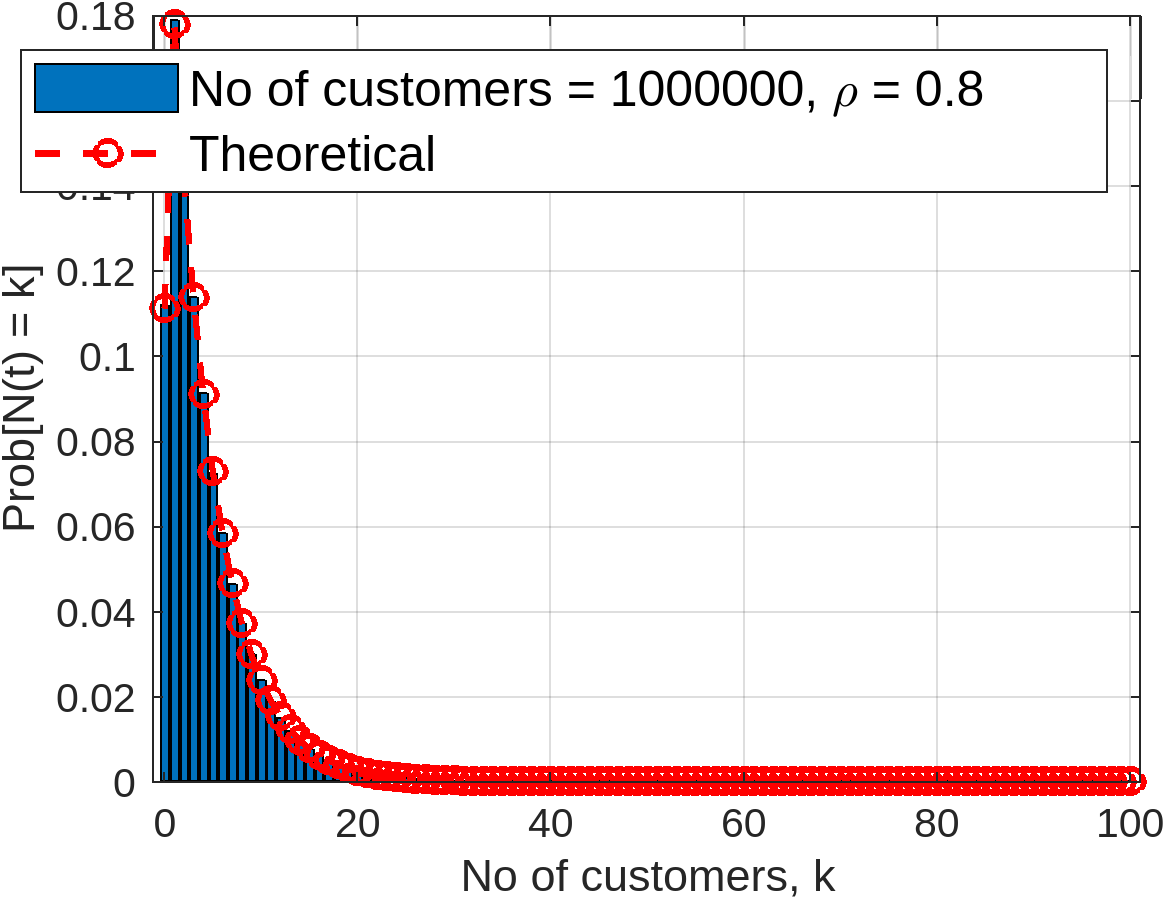
\includegraphics[width=200px]{../code/figures/N_PMF/semilogy_plot_no_customers_1000000_rho_0.8.png}
  }
  \subfloat[]{
    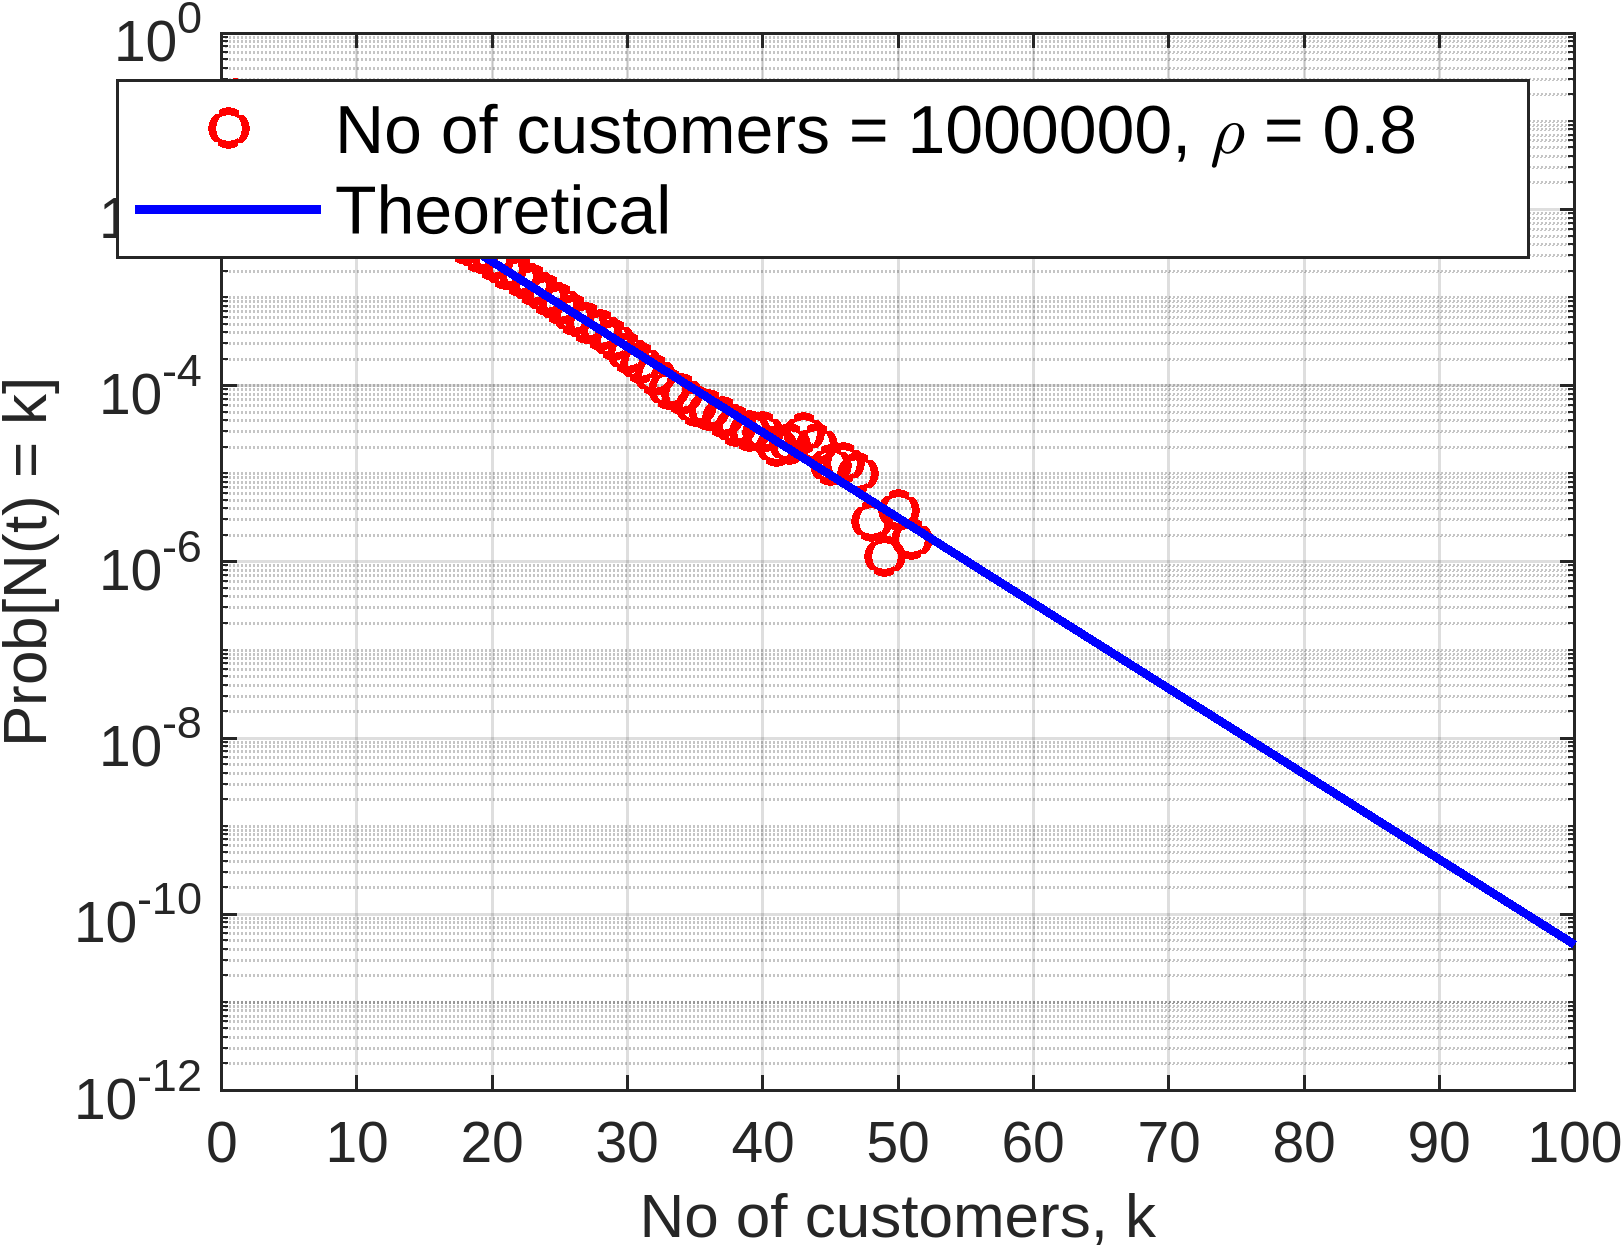
\includegraphics[width=200px]{../code/figures/N_PMF/bar_plot_no_customers_1000000_rho_0.8.png}
  }
  \hspace{0px}
  \subfloat[]{
    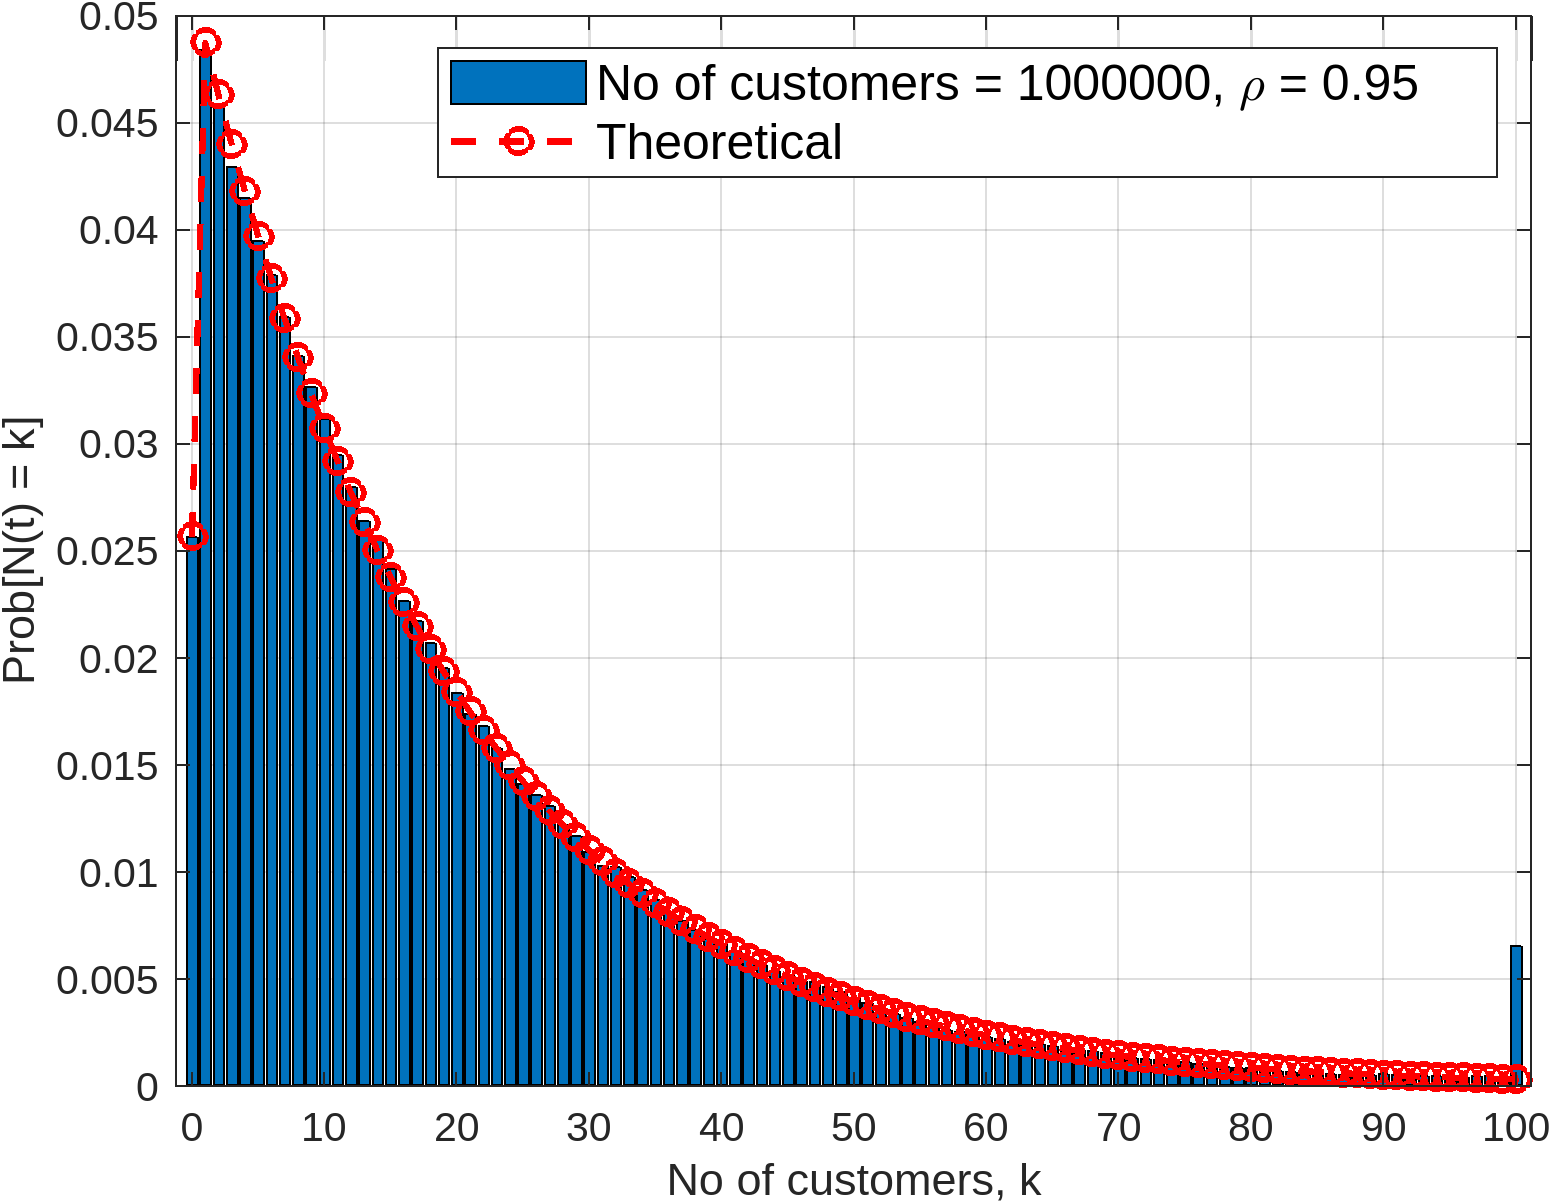
\includegraphics[width=200px]{../code/figures/N_PMF/semilogy_plot_no_customers_1000000_rho_0.95.png}
  }
  \subfloat[]{
    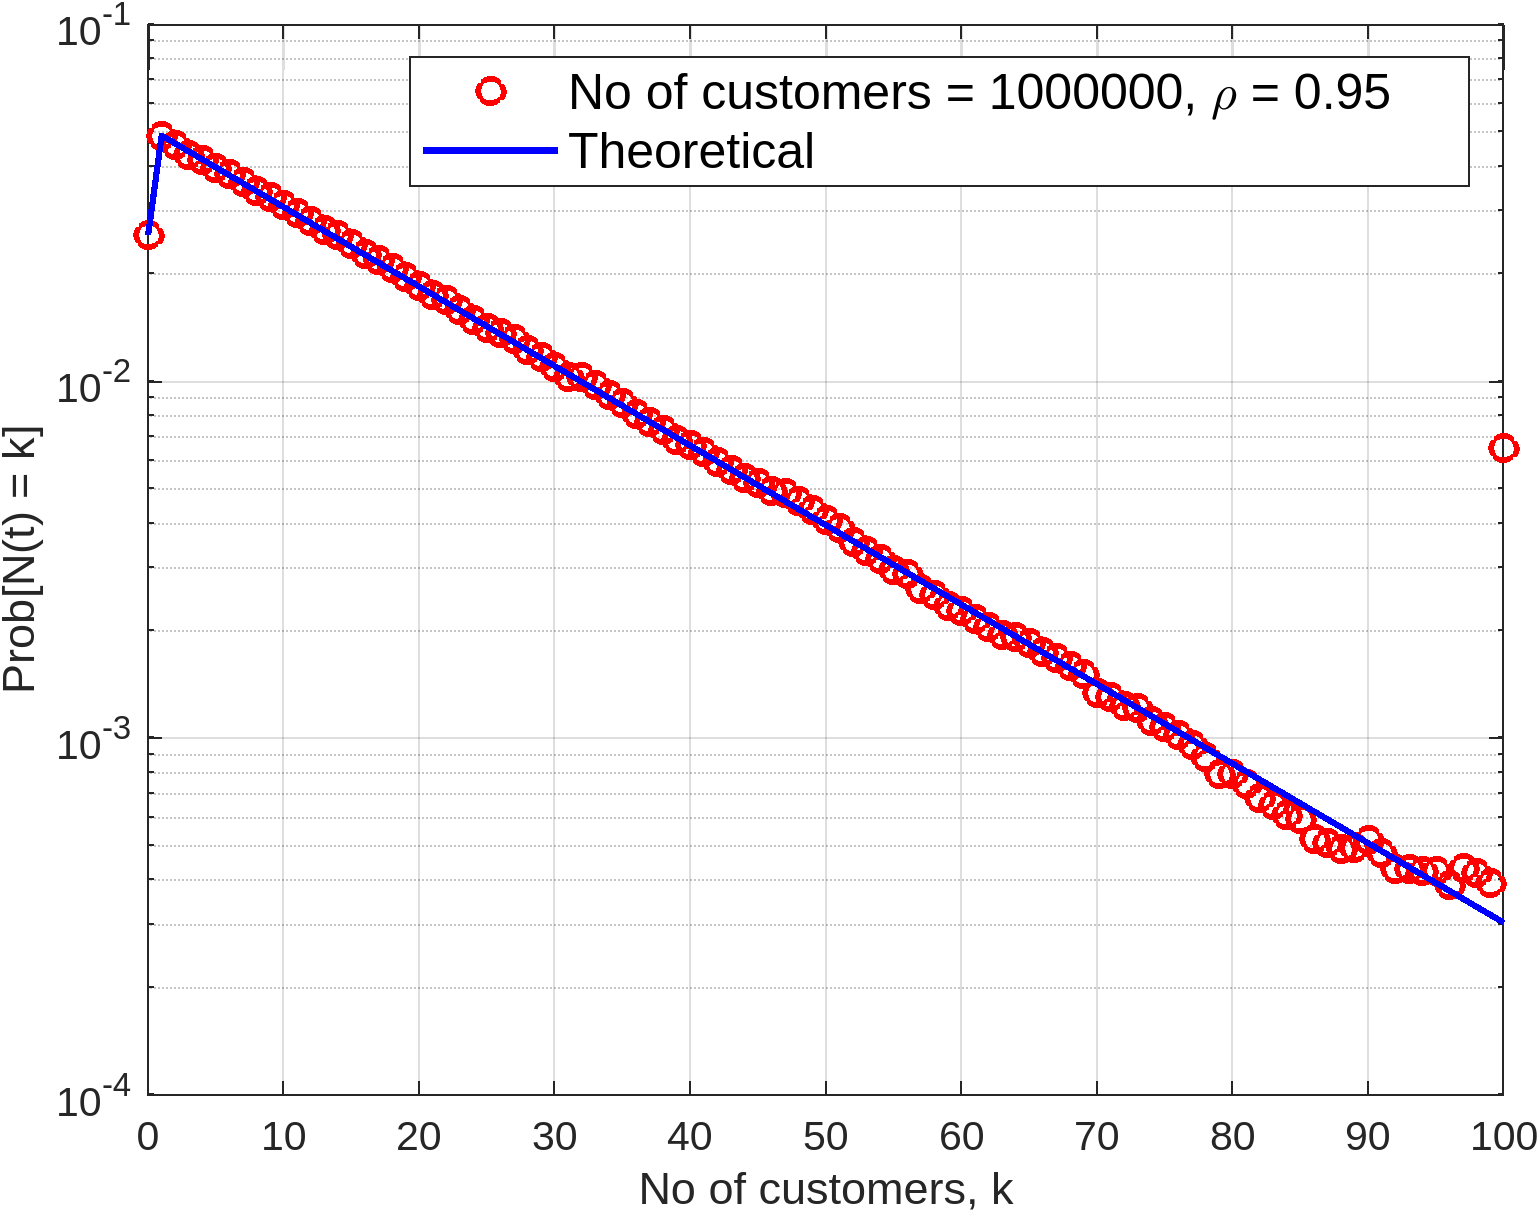
\includegraphics[width=200px]{../code/figures/N_PMF/bar_plot_no_customers_1000000_rho_0.95.png}
  }
  \caption{PMF of $N(t)$  for high traffic intensity and 1000000 customers}  
  \label{PMF_N_high_more_cust}
\end{figure}

\subsection{Prob$[W > 0]$ vs $c$}
\begin{figure}
  \centering 
  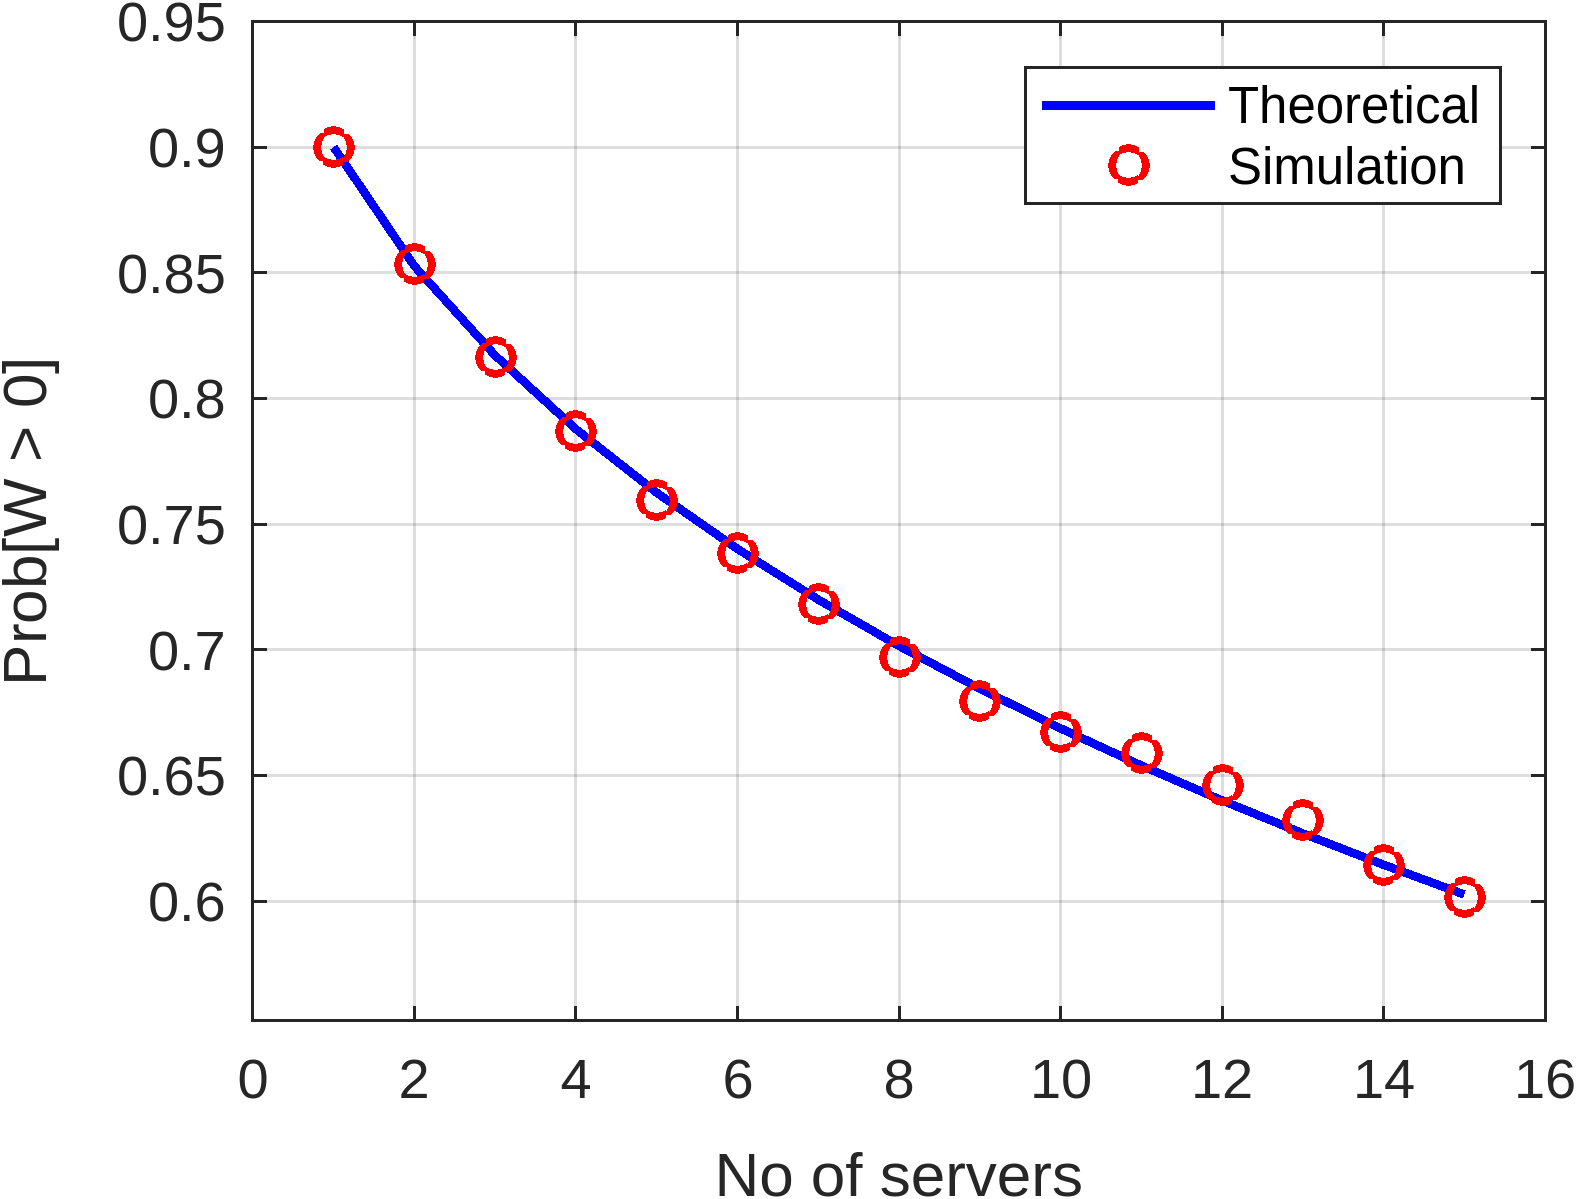
\includegraphics[width=250px]{../code/figures/pWaiting_vs_c/no_customers_1000000_max_c_15.png}
  \caption{Prob$[W > 0]$ vs $c$ for $\rho=0.9$}
  \label{W_vs_c}
\end{figure}

Figure \ref{W_vs_c} shows the probability having to wait as function of the number of servers 
in the system for a fixed traffic intensity. The plot indicates that probability of having to 
decrease as the number of the servers increase, which is intuitive since more servers means 
less waiting time and hence the probability of having to wait decreases. Furthermore, the 
empirical curve agrees with theoretical one.

\section{Conclusion}


\newpage
\section*{Appendix}
\footnotesize
\begin{lstlisting}[style=Matlab-editor, basicstyle=\ttfamily\footnotesize]
  function [DT, startList, serviceTime] = simulation_loop(AT, ST, c)
  numCustomers = length(AT);
  startList = zeros(1, numCustomers);
  DT = zeros(1, numCustomers);
  serverList = zeros(1, c); % Initialize server list with c free servers
  serverID = zeros(1, numCustomers);
  serviceTime = zeros(1, c);
  % Run simulation
  for i = 1:numCustomers
      % Find the earliest available server
      [~, idx] = min(serverList);
      earliestAvailableTime = serverList(idx);
      serverID(i) = idx;
      
      % Calculate the start time for the customer
      startTime = max(AT(i), earliestAvailableTime);
      startList(i) = startTime;
      
      % Calculate the departure time
      departureTime = startTime + ST(i);
      DT(i) = departureTime;
      
      % Update the server list
      serverList(idx) = departureTime;
      serviceTime(idx) = serviceTime(idx) + ST(i); 
  end
end
\end{lstlisting}

\end{document}
